\chapter{Results and Discussion}
\label{chap:results}
This chapter presents the main results and findings from all experiments defined in the previous Chapter \ref{ch:experiments}. First a short revisit of the results from the Best Channel Study is given, as the best channels are used in the further experiments.

The main results of this thesis begin with the three Benchmarks, to test the PatchTST classifiers ability to generalize to unseen dataset domains. Benchmark 1 assigns the testset over all domains, Benchmark 2 to specific \texttt{rod\_type + tolerance} domains and Benchmark 3 assigns the testset individually to all domain-attributes for a broader held-out testset.

After the Benchmark results follow the results from the Deviation Analysis I and II, which aim to investigate how certain deviations applied to the insertions, affect physical success outcome, and which deviations produce ambiguous insertion signals that confuse the models ability to classify correctly.

In the end a summary of the main findings is given.



\section{Best Channel Study}
\label{sec:results_best_channel}
The Best Channel Study was conducted as a standalone study as the first Experiment in Section \ref{sec:exp1_best_channel_study} with its own Motivation, Methods, Results, Discussion and Conclusion.
The recorded dataset contains these signal modalities: force/torque, TCP pose, TCP velocity, joint pose, joint velocity, tool acceleration, per-joint current consumption, and temperature readings per joint.

Stage 1 evaluated each individual channel group with the \texttt{Base} PatchTST model and selected force/torque, TCP pose, joint velocity and current consumption as the strongest signals based on validation balanced accuracy. Refer to \figref{fig:best_channel_single_val_bal_acc} and \figref{fig:best_channel_single_val_loss} in Section \ref{sec:best_channel_study_results} for the detailed comparison.

Stage 2 combined the selected channel groups in all $4\times4=16$ possible ways, with training being done with the \texttt{Big} PatchTST model, in order to better represent the higher dimensional and information rich data in latent space. All $16$ tested channel combinations are shown in an odered binary counting pattern in \figref{fig:results_BCS_comparison}. Light blue highlighted rows mark the single channel groups. \tabref{tab:best_channels_in_detail} shows the validation balanced accuracy from the selected best channels individually and as a combined group.

The best channel study shows that FT is the strongest individual channel group based on mean validation balanced accuracy in \tabref{tab:best_channels_in_detail}, but that the highest performance is obtained when FT is combined with additional robot-state modalities. In particular, current, TCP pose, and joint velocity provide complementary information about actuator load, geometric state, and motion dynamics. Based on these results, the combination of F/T, TCP pose, joint velocity, and current is used for the following benchmark experiments.

\begin{figure}[htpb]
    \centering
    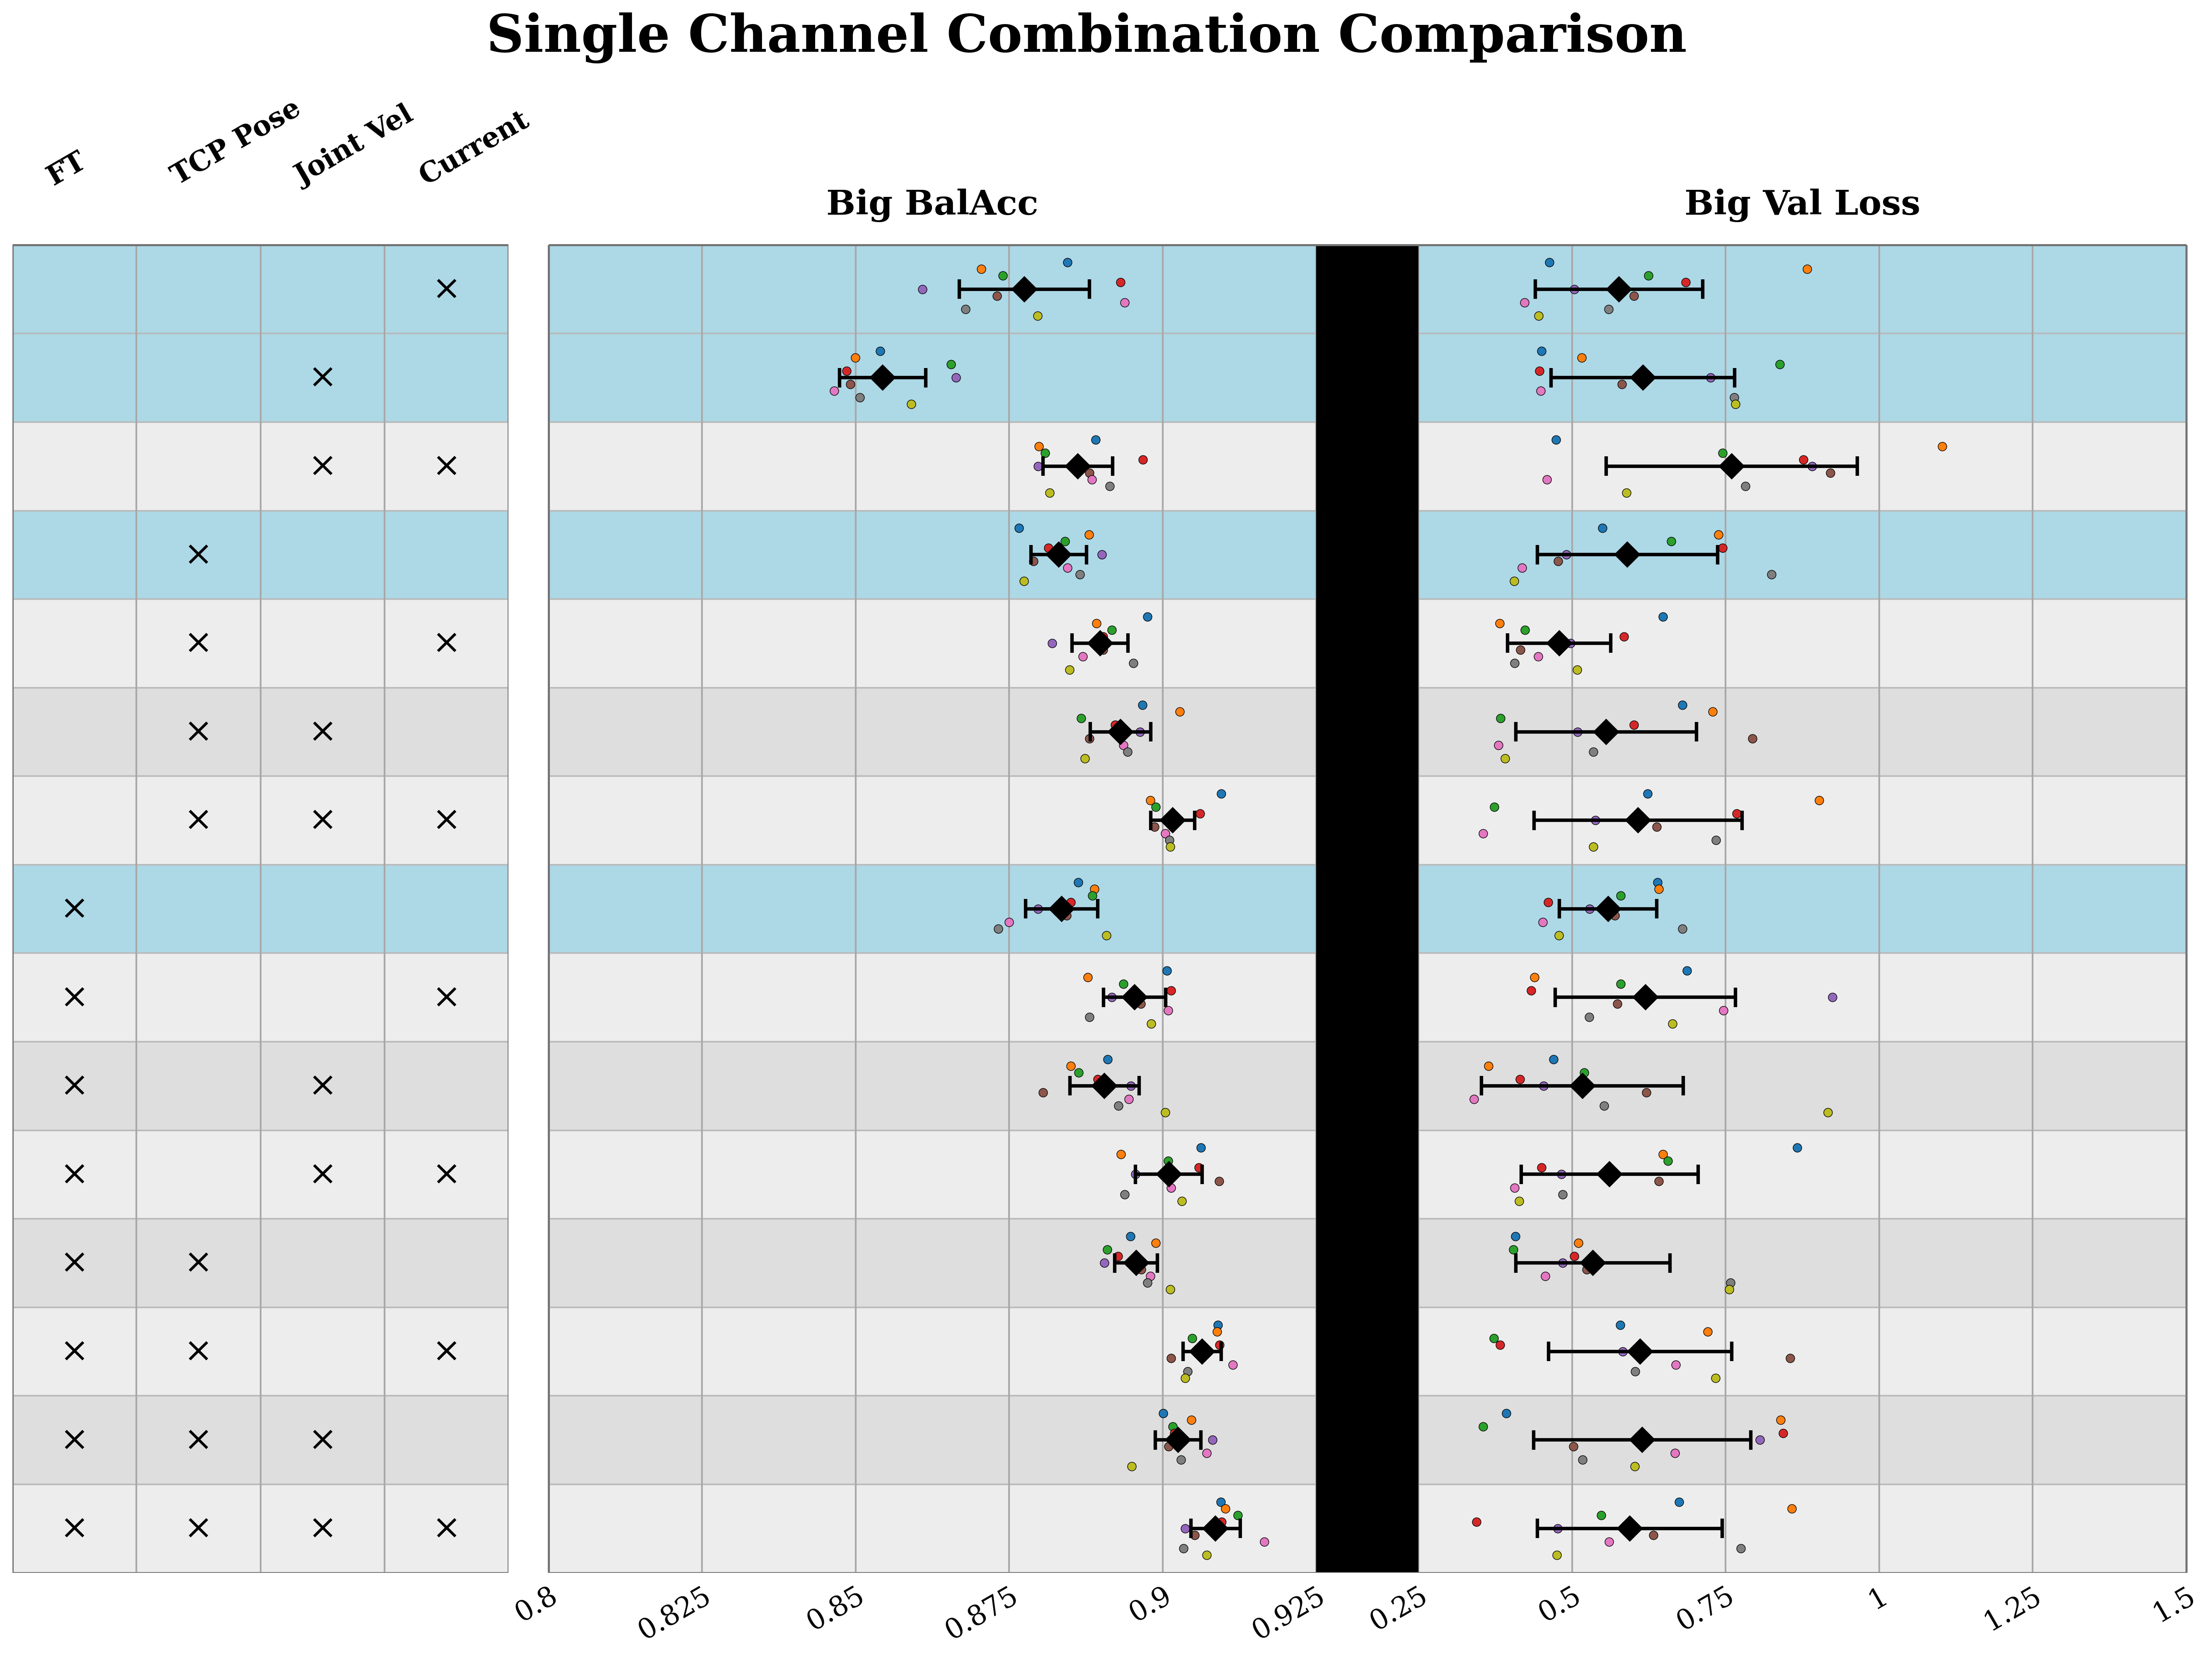
\includegraphics[width=1.0\textwidth]{chapters/7-results/best_channel_study/channel_matrix_plot.png}
    \caption{All combinations of the selected best channels evaluated with the \texttt{Big} model on validation balanced accuracy and validation loss across the 9 training run seed combinations. Rows highlighted in light blue mark the single channel groups.}
    \label{fig:results_BCS_comparison}
\end{figure}

\begin{table}[htbp]
    \centering
    \caption{Best channels selected with detailed view on validation balanced accuracy across the 9 training runs. ms: model seed, ss: split seed.}
    \label{tab:best_channels_in_detail}
    \begin{tabular}{llll}
        \toprule
        \textbf{Channel} & \textbf{Mean $\pm$ std} & \textbf{Min (ms, ss)} & \textbf{Max (ms, ss)}\\
        \midrule

        \texttt{FT} & 0.8859 $\pm$ 0.0075 & 0.8716 (420,69) & 0.8930 (420,420)\\
        \texttt{TCP\_POS} & 0.8854 $\pm$ 0.0053 & 0.8782 (42,42) & 0.8932 (69,69) \\
        \texttt{JOINT\_VEL} & 0.8535 $\pm$ 0.0083 & 0.8447 (420,42) & 0.8667 (69,69) \\
        \texttt{CURRENT} & 0.8792 $\pm$ 0.0125 & 0.8607 (69,69) & 0.8974 (420,42) \\
        \texttt{FT} + \texttt{TCP\_POS} + \texttt{JOINT\_VEL} + \texttt{CURRENT} & 0.9139 $\pm$ 0.0047 & 0.9081 (420,69) & 0.9227 (420,42)\\
        \bottomrule
    \end{tabular}
\end{table}


\newpage
\section{Benchmark 1: Test on Mixed Split}
\label{sec:results_benchmark1}
Benchmark 1 evaluates the selected channel configuration under an in-distribution split, where the test samples are unseen insertion attempts but originate from the same overall experimental domain as the training data. This testset is evaluated on the
\begin{itemize}
    \item Base config: \texttt{Base} PatchTST model with \texttt{FT} as the only input data and
    \item Big config: \texttt{Big} PatchTST model with the best channels \texttt{FT + TCP\_POS + JOINT\_VEL + CURRENT} as input data.
\end{itemize}

The test balanced accuracy (TBA) in \figref{fig:bm1_test_result} (a) is high for both model variants. The Base config reaches a mean TBA of 0.8617, while the Big config reaches 0.8909 (\tabref{tab:bm1_bal_acc_detail}). Across the evaluated seed combinations, the Big config achieves higher balanced accuracy in all runs.

The test loss in \figref{fig:bm1_test_result} (b) shows a different pattern. The Base config has a lower mean test loss and a smaller spread across seeds, while the Big config shows a higher mean loss and larger variability. Thus, Benchmark 1 shows a clear advantage of the Big config in test balanced accuracy, but not in test loss.

The number of sequences and class balance of the training, validation and test split is shown in \tabref{tab:bm1_data_split}.
\begin{figure}[htbp]
    \centering
    \begin{subfigure}[t]{0.49\textwidth}
        \centering
        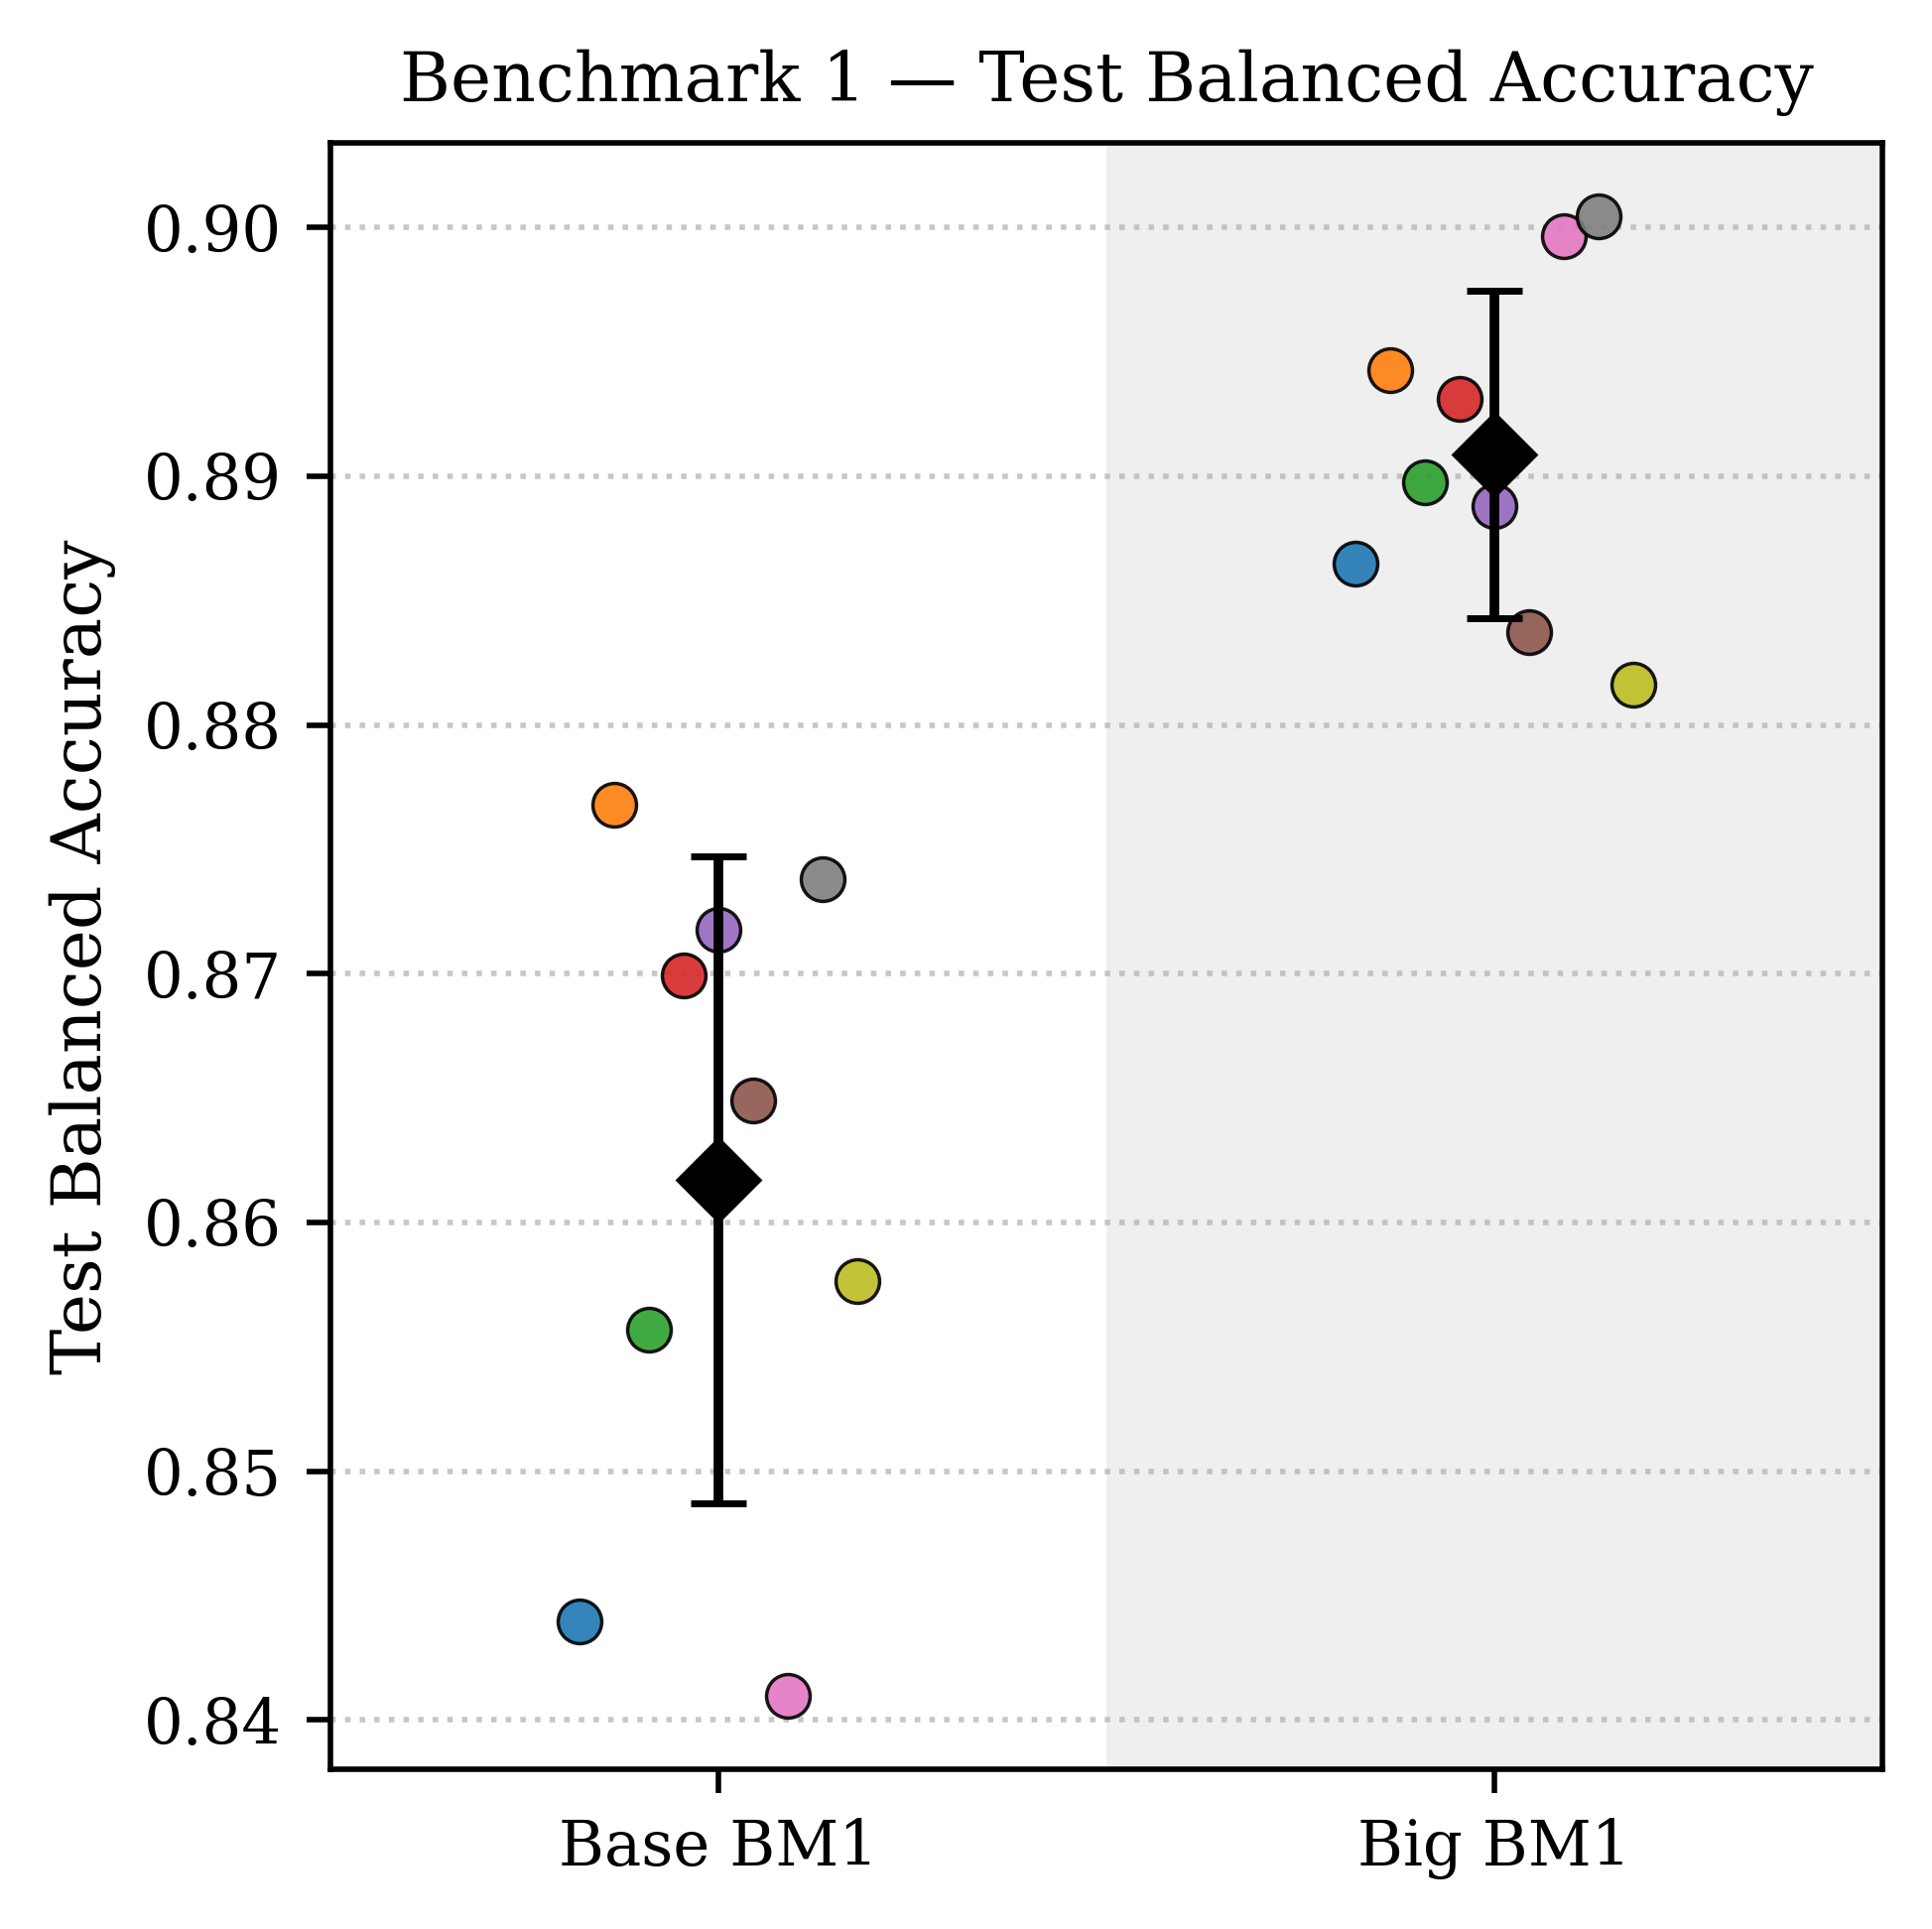
\includegraphics[width=0.9\textwidth]{chapters/7-results/bm1/bm1_bal_acc.png}
        \caption{}
    \end{subfigure}
    \begin{subfigure}[t]{0.49\textwidth}
        \centering
        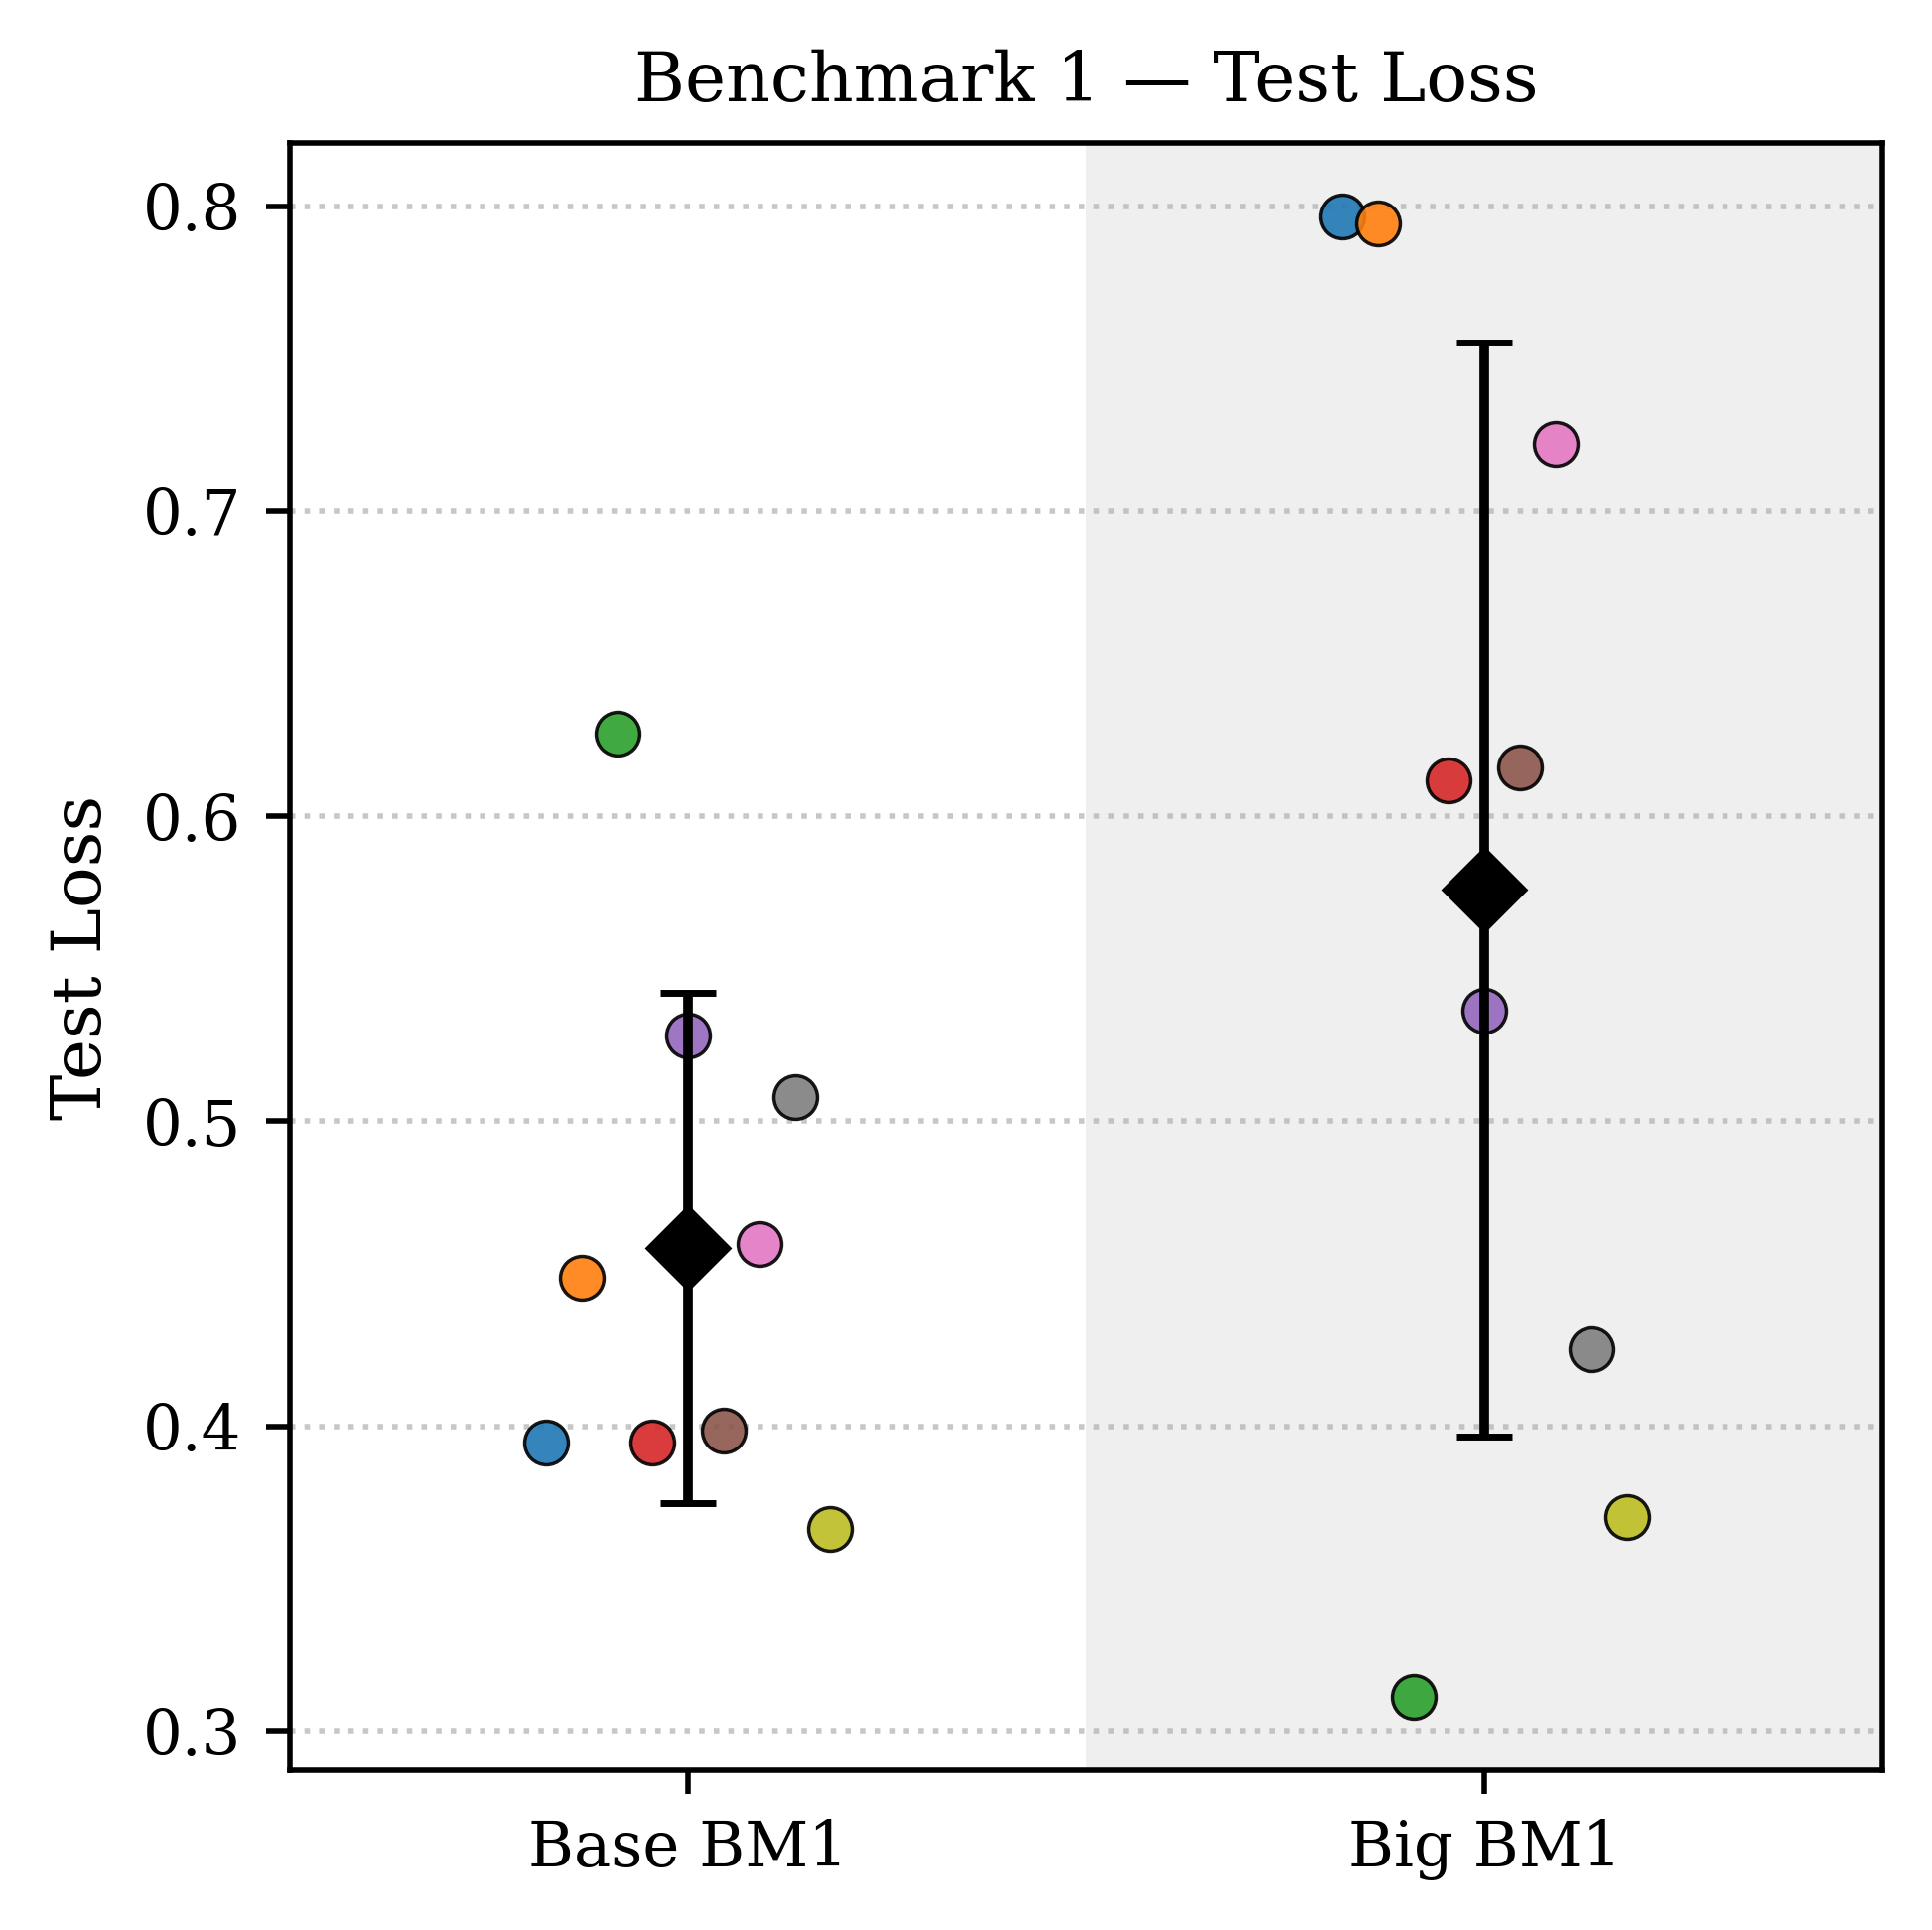
\includegraphics[width=0.9\textwidth]{chapters/7-results/bm1/bm1_test_loss.png}
        \caption{}
    \end{subfigure}
    \caption{Benchmark 1 results. (a) Test balanced accuracy with direct comparison of the Base config consisting of the \texttt{Base} PatchTST model on \texttt{FT} only and the Big config with the \texttt{Big} PatchTST model on the best channels.}
    \label{fig:bm1_test_result}
\end{figure}

\begin{table}[htbp]
    \centering
    \caption{Test balanced accuracy detailed results of Benchmark 1.}
    \label{tab:bm1_bal_acc_detail}
    \begin{tabular}{llll}
        \toprule
        \textbf{Domain} & \textbf{Mean $\pm$ std} & \textbf{Min (ms, ss)} & \textbf{Max (ms, ss)}\\
        \midrule

        \texttt{Base BM1} & 0.8617 $\pm$ 0.0130 & 0.8410 (420, 42) & 0.8768 (42, 69)\\
        \texttt{Big BM1} & 0.8909 $\pm$ 0.0066 & 0.8816 (420, 420) & 0.9004 (420, 69) \\
        \bottomrule
    \end{tabular}
\end{table}

\begin{table}[htbp]
    \centering
    \caption{Exact Train, Validation, Test splits with class balance for Benchmark 1.}
    \label{tab:bm1_data_split}
    \begin{tabular}{lll}
        \toprule
        \textbf{Training (pos, neg)} & \textbf{Validation (pos, neg)} & \textbf{Test (pos, neg)}\\
        \midrule

        5852 (3173, 2679) & 1033 (560, 473) & 1215 (659, 556)\\
        \bottomrule
    \end{tabular}
\end{table}

\section{Benchmark 2: Test on Individual Hole}
\label{sec:results_benchmark2}

Benchmark 2 evaluates the model on unseen hole domains. The exact train, validation, and test splits are listed in \tabref{tab:bm2_data_split}, with each held-out domain containing either 820 ($820 = 100 + 360 + 360$) or 1060 ($1060 = 100 + 480 + 480$) test samples with both classes represented.

The detailed test balanced accuracy values are reported in \tabref{tab:bm2_bal_acc_detail} and visualized in \figref{fig:bm2_test_bal_acc_result}. Both configs reach balanced accuracies above 0.80 for most held-out domains. The Big config achieves higher mean balanced accuracy than the Base config in all evaluated domains. The highest results are obtained for \texttt{BM2\_small\_3}, \texttt{BM2\_rect\_2}, and \texttt{BM2\_rect\_3}, while \texttt{BM2\_rect\_1} is the only domain with a clearly lower balanced accuracy.

The test loss values in \figref{fig:bm2_test_loss_result} also identify \texttt{BM2\_rect\_1} as the most difficult held-out domain. This domain shows the highest loss values and the largest spread across seeds, especially for the Big config. For the remaining domains, the loss values are lower and less spread.

Overall, Benchmark 2 shows that the Big config performs best in terms of balanced accuracy, but that performance varies noticeably between the individual held-out hole domains.

\begin{figure}[htbp]
    \centering
    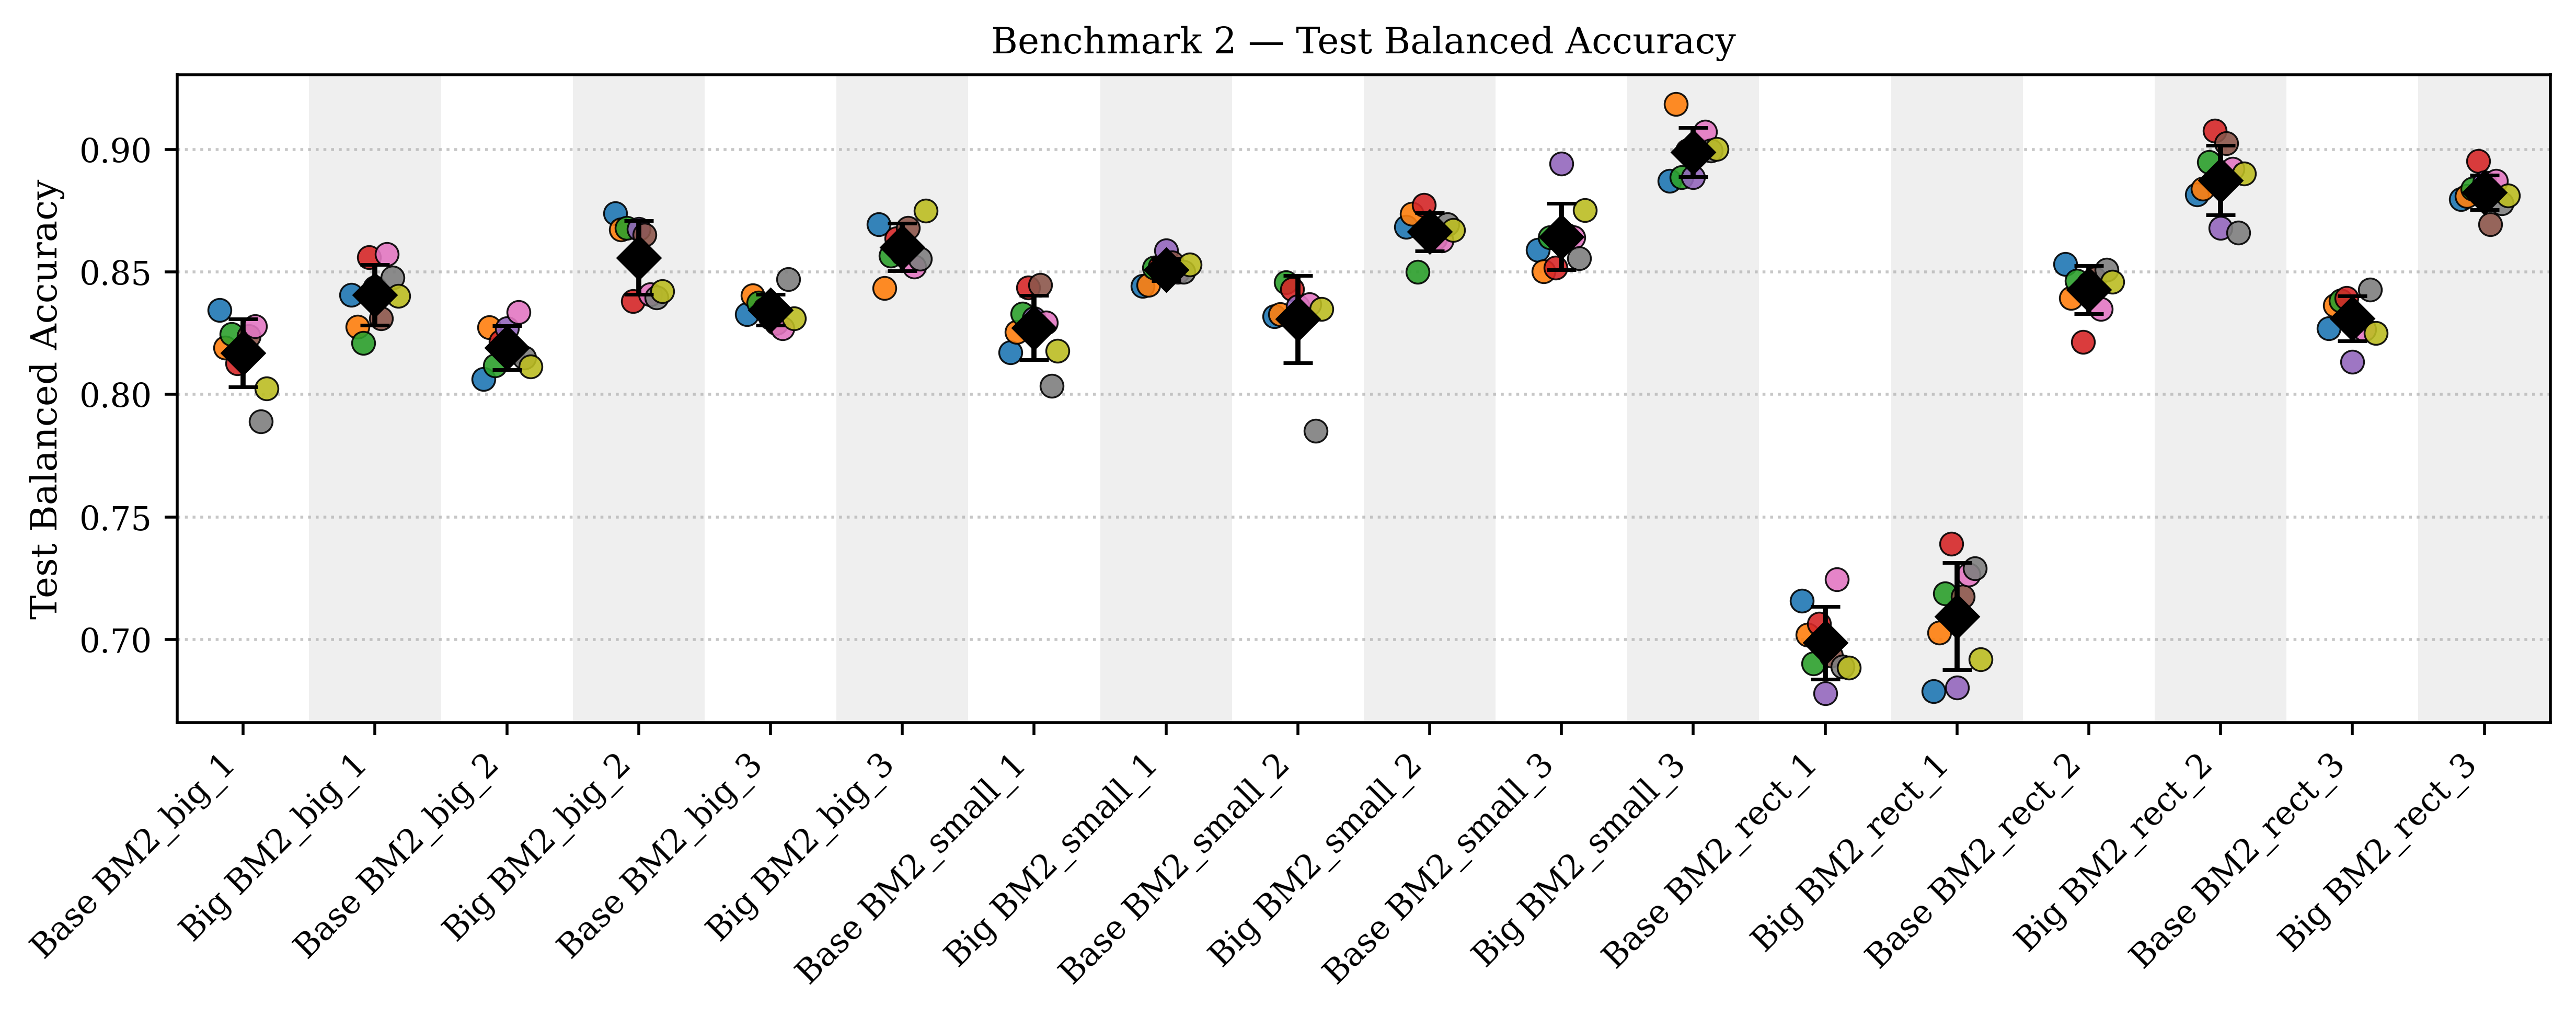
\includegraphics[width=1.0\linewidth]{chapters/7-results/bm2/bm2_test_bal_acc.png}
    \caption{Test balanced accuracy of all of all hole domains specified in \tabref{tab:bm2_domains} evaluated on both the Base and Big config.}
    \label{fig:bm2_test_bal_acc_result}
\end{figure}

\begin{figure}[htbp]
    \centering
    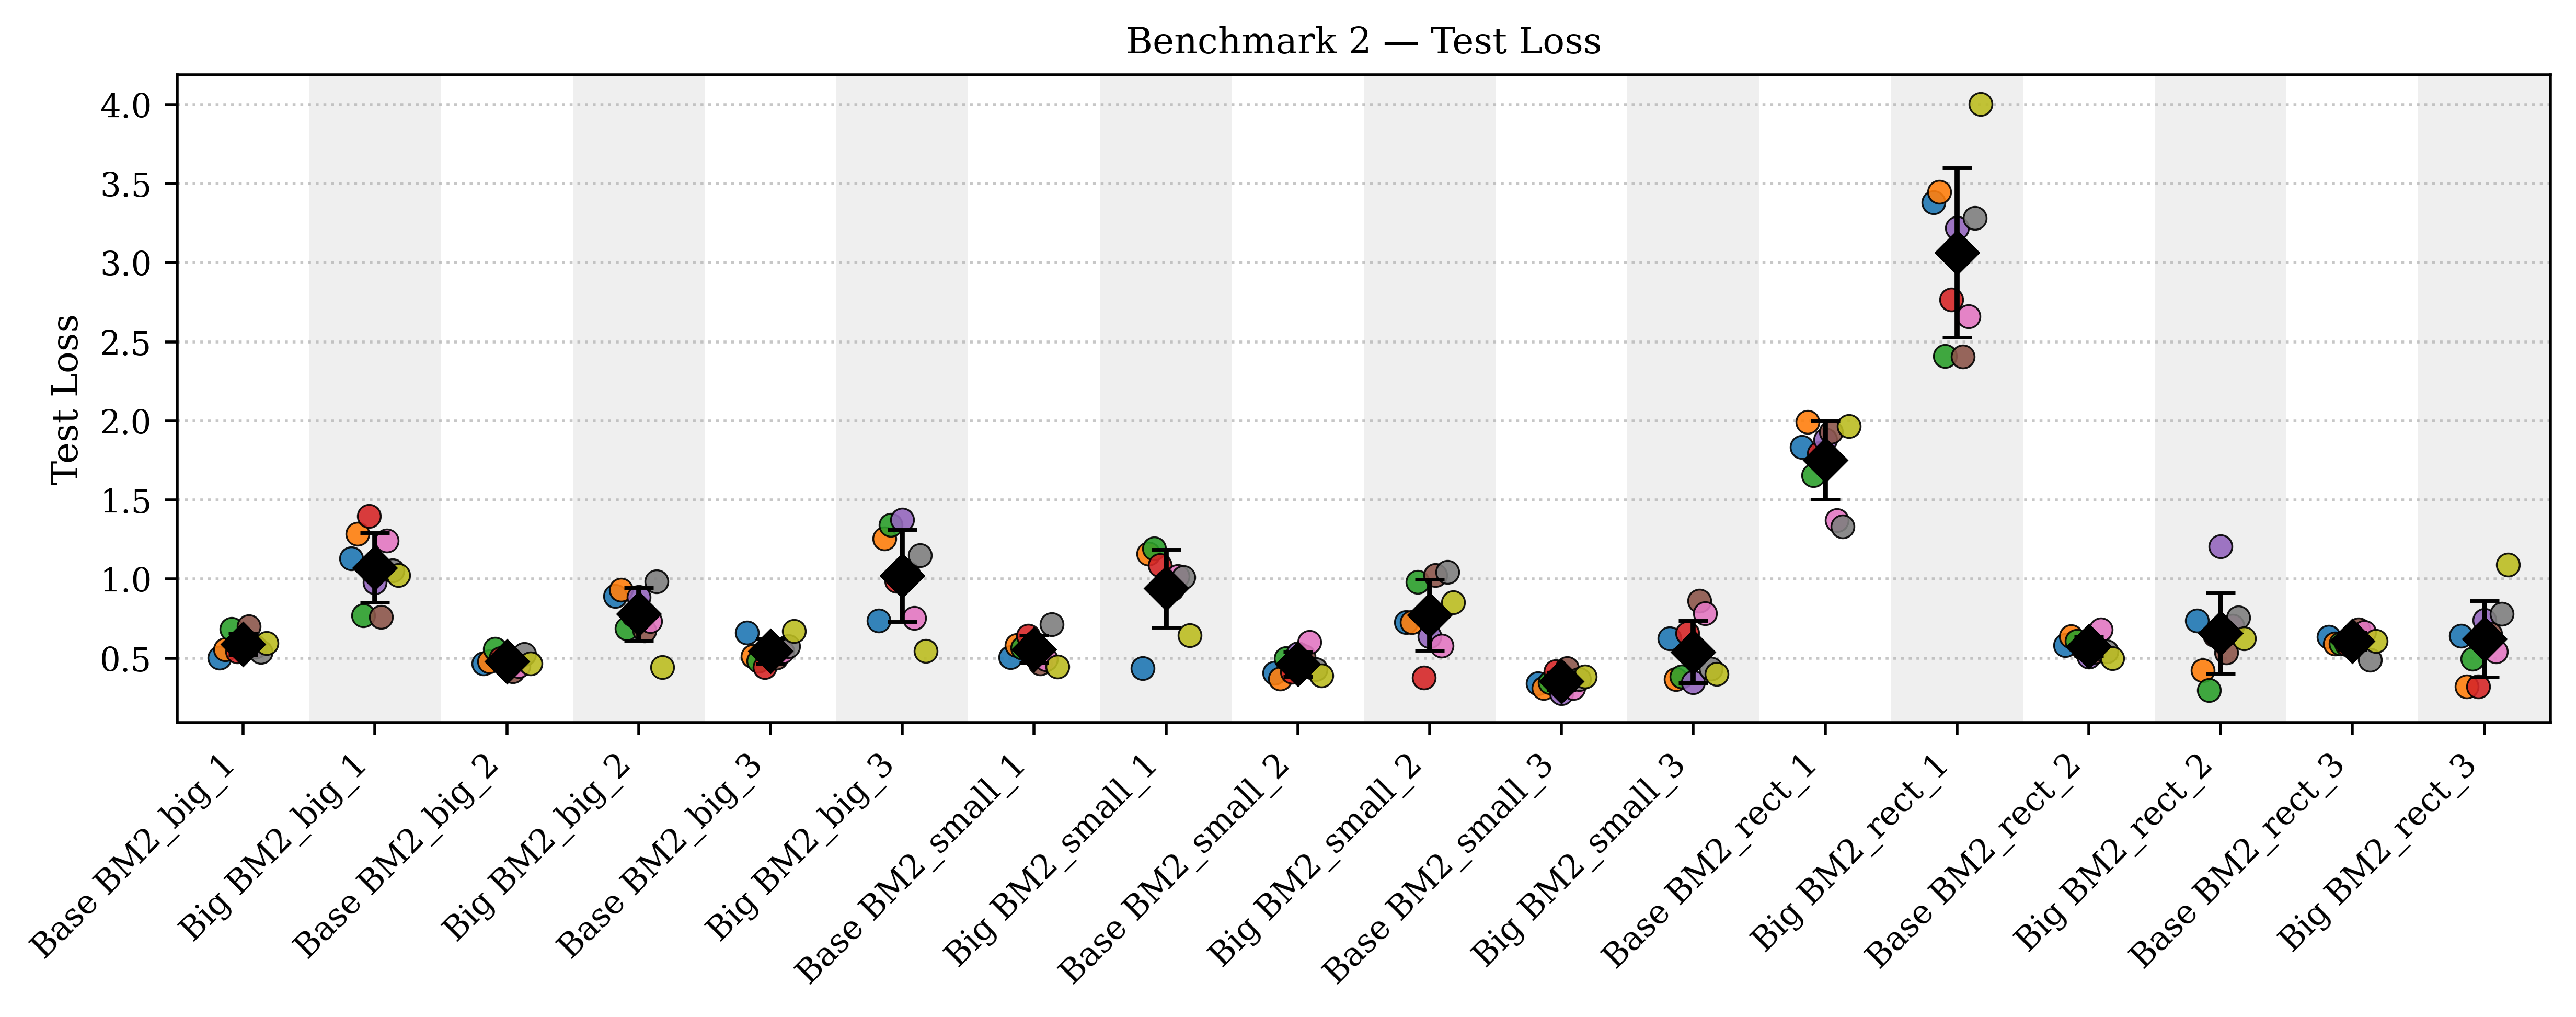
\includegraphics[width=1.0\linewidth]{chapters/7-results/bm2/bm2_test_loss.png}
    \caption{Test loss of all of all hole domains specified in \tabref{tab:bm2_domains} evaluated on both the Base and Big config.}
    \label{fig:bm2_test_loss_result}
\end{figure}


\begin{table}[htbp]
    \centering
    \caption{Test balanced accuracy detailed results of Benchmark 2. Rows in bold show the highest test balanced accuracy, while underlined rows show the lowest test balanced accuracy.}
    \label{tab:bm2_bal_acc_detail}
    \begin{tabular}{llll}
        \toprule
        \textbf{Domain} & \textbf{Mean $\pm$ std} & \textbf{Min (ms, ss)} & \textbf{Max (ms, ss)}\\
        \midrule 

        \texttt{Base BM2\_big\_1} & \underline{0.8169} $\pm$ \underline{0.0139} & \underline{0.7889 (420, 69)} & \underline{0.8344 (42, 42)}\\
        \texttt{Big BM2\_big\_1} & 0.8406 $\pm$ 0.0124 & 0.8209 (42, 420) & 0.8573 (420, 42) \\
        \texttt{Base BM2\_big\_2} & 0.8190 $\pm$ 0.0090 & 0.8062 (42, 42) & 0.8336 (420, 42)\\
        \texttt{Big BM2\_big\_2} & 0.8558 $\pm$ 0.0151 & 0.8381 (69, 42) & 0.8739 (42, 42) \\
        \texttt{Base BM2\_big\_3} & 0.8345 $\pm$ 0.0062 & 0.8270 (420, 42) & 0.8469 (420, 69)\\
        \texttt{Big BM2\_big\_3} & 0.8601 $\pm$ 0.0097 & 0.8435 (42, 69) & 0.8749 (420, 420) \\
        \midrule
        \texttt{Base BM2\_small\_1} & 0.8272 $\pm$ 0.0131 & 0.8034 (420, 69) & 0.8446 (69, 420)\\
        \texttt{Big BM2\_small\_1} & 0.8509 $\pm$ 0.004 & 0.8442 (42, 42) & 0.8588 (69, 69) \\
        \texttt{Base BM2\_small\_2} & 0.8308 $\pm$ 0.0178 & 0.7850 (420, 69) & 0.8458 (42, 420)\\
        \texttt{Big BM2\_small\_2} & 0.8664 $\pm$ 0.0077 & 0.8499 (42, 420) & 0.8774 (69, 42) \\
        \texttt{Base BM2\_small\_3} & 0.8643 $\pm$ 0.0136 & 0.8502 (42, 69) & 0.8942 (69, 69)\\
        \texttt{Big BM2\_small\_3} & \textbf{0.8988} $\pm$ \textbf{0.0100} & \textbf{0.8872 (42, 42)} & \textbf{0.9184 (42, 69)} \\
        \midrule
        \texttt{Base BM2\_rect\_1} & \underline{0.6986} $\pm$ \underline{0.0148} & \underline{0.6779 (69, 69)} & \underline{0.7246 (420, 42)}\\
        \texttt{Big BM2\_rect\_1} & 0.7094 $\pm$ 0.0219 & 0.6789 (42, 42) & 0.7391 (69, 42) \\
        \texttt{Base BM2\_rect\_2} & 0.8427 $\pm$ 0.0097 & 0.8214 (69, 42) & 0.8532 (42, 42)\\
        \texttt{Big BM2\_rect\_2} & \textbf{0.8874} $\pm$ \textbf{0.0141} & \textbf{0.8661 (420, 69)} & \textbf{0.9076 (69, 42)} \\
        \texttt{Base BM2\_rect\_3} & 0.8310 $\pm$ 0.0092 & 0.8132 (69, 69) & 0.8427 (420, 69)\\
        \texttt{Big BM2\_rect\_3} & \textbf{0.8824} $\pm$ \textbf{0.0071} & \textbf{0.8695 (69, 420)} & \textbf{0.8951 (69, 42)} \\
        \bottomrule
    \end{tabular}
\end{table}

\begin{table}[htbp]
    \centering
    \caption{Exact Train, Validation, Test splits with class balance for Benchmark 2.}
    \label{tab:bm2_data_split}
    \begin{tabular}{llll}
        \toprule
        \textbf{Domain} & \textbf{Training (pos, neg)} & \textbf{Validation (pos, neg)} & \textbf{Test (pos, neg)}\\
        \midrule

        \texttt{BM2\_big\_1} & 5984 (3254, 2730) & 1056 (574, 482) & 1060 (564, 496)\\
        \texttt{BM2\_big\_2} & 6188 (3350, 2838) & 1092 (591, 501) & 820 (451, 369)\\
        \texttt{BM2\_big\_3} & 6188 (3365, 2823) & 1092 (594, 498) &  820 (433, 387)\\
        
        \texttt{BM2\_small\_1} & 5984 (3199, 2785) & 1056 (565, 491) & 1060 (628, 432)\\
        \texttt{BM2\_small\_2} & 6188 (3296, 2892) & 1092 (582, 510) & 820 (514, 306)\\
        \texttt{BM2\_small\_3} & 6188 (3397, 2791) & 1092 (600, 492) & 820 (395, 425)\\

        \texttt{BM2\_rect\_1} & 5984 (3290, 2694) & 1056 (581, 475) & 1060 (521, 539)\\
        \texttt{BM2\_rect\_2} & 6188 (3343, 2845) & 1092 (590, 502) & 820 (459, 361)\\
        \texttt{BM2\_rect\_3} & 6188 (3370, 2818) & 1092 (595, 497) & 820 (427, 393)\\
        \bottomrule
    \end{tabular}
\end{table}

\section{Benchmark 3: Test on Held-Out Group}
\label{sec:results_benchmark3}

Benchmark 3 evaluates generalization to held-out domain groups. The exact train, validation, and test splits are listed in \tabref{tab:bm3_data_split}. Depending on the held-out domain, the test sets contain between 900 and 3600 samples, with both success and failure samples represented in all cases.

The detailed test balanced accuracy results are reported in \tabref{tab:bm3_bal_acc_detail}. Across all held-out domain groups, the Big config achieves a higher mean TBA than the Base config. For \texttt{BM3\_batch\_1} however, this difference is small, but more significant for other domains, especially for the rectangular rod and gripper domains.

The results for the held-out \texttt{batch} domains are shown in \figref{fig:bm3_batch_test_bal_acc}, there the test balanced accuracy is lower than for most other domain groups. The Big config reaches mean balanced accuracies of 0.6781, 0.7083, and 0.7691 for \texttt{BM3\_batch\_1}, \texttt{BM3\_batch\_2}, and \texttt{BM3\_batch\_3}, respectively. The largest seed-dependent spread is observed for \texttt{BM3\_batch\_1}.

For the held-out \texttt{rod\_type} domains the results in \figref{fig:bm3_rod_type_test_bal_acc} show that the Big config reaches similar results for \texttt{BM3\_big} and \texttt{BM3\_small}, with mean balanced accuracies of 0.8246 and 0.8265. The held-out \texttt{BM3\_rect} domain has lower mean TBA than the other rod domains, however the improvement of the Big config over the Base config of $0.7507 - 0.6834 = 0.0673$ mean TBA points is the highest in the entire Benchmark.

The highest TBA results of Benchmark 3, in \figref{fig:bm3_tolerance_test_bal_acc}, are obtained by the held-out tolerance domains. The Big config reaches a mean TBA of 0.7980 for \texttt{BM3\_tol\_1}, 0.8698 for \texttt{BM3\_tol\_2}, with 0.8798 for \texttt{BM3\_tol\_3} being the highest mean TBA achieved in the entire Benchmark. These domains also show comparatively small standard deviations across seed combinations.

The results for the held-out \texttt{gripper\_type} domains in \figref{fig:bm3_gripper_type_test_bal_acc} show that the Big config reaches mean TBAs of 0.7735 for \texttt{BM3\_round}, 0.7122 for \texttt{BM3\_rect\_gripper}, and 0.7691 for \texttt{BM3\_flat}. The rectangular gripper condition is therefore the lowest-performing gripper-domain result, with \texttt{BM3\_rect\_gripper} on Base config achieving the lowest mean TBA in the entire Benchmark.

The summarized Big config results in \figref{fig:bm3_all_domains_test_bal_acc} show the same ordering across domain groups. The highest test balanced accuracies are obtained for the held-out \texttt{tolerance} domains, followed by the \texttt{big} and \texttt{small} \texttt{rod\_type} domains. The lowest results occur in the held-out \texttt{batch} domains and in the \texttt{BM3\_rect\_gripper} domain. The corresponding test loss plots are provided in \appref{app:bm3_loss}; they show higher loss values for the lower-performing domains, especially in the \texttt{batch} and \texttt{BM3\_rect\_gripper} cases.

\begin{figure}[htbp]
    \centering
    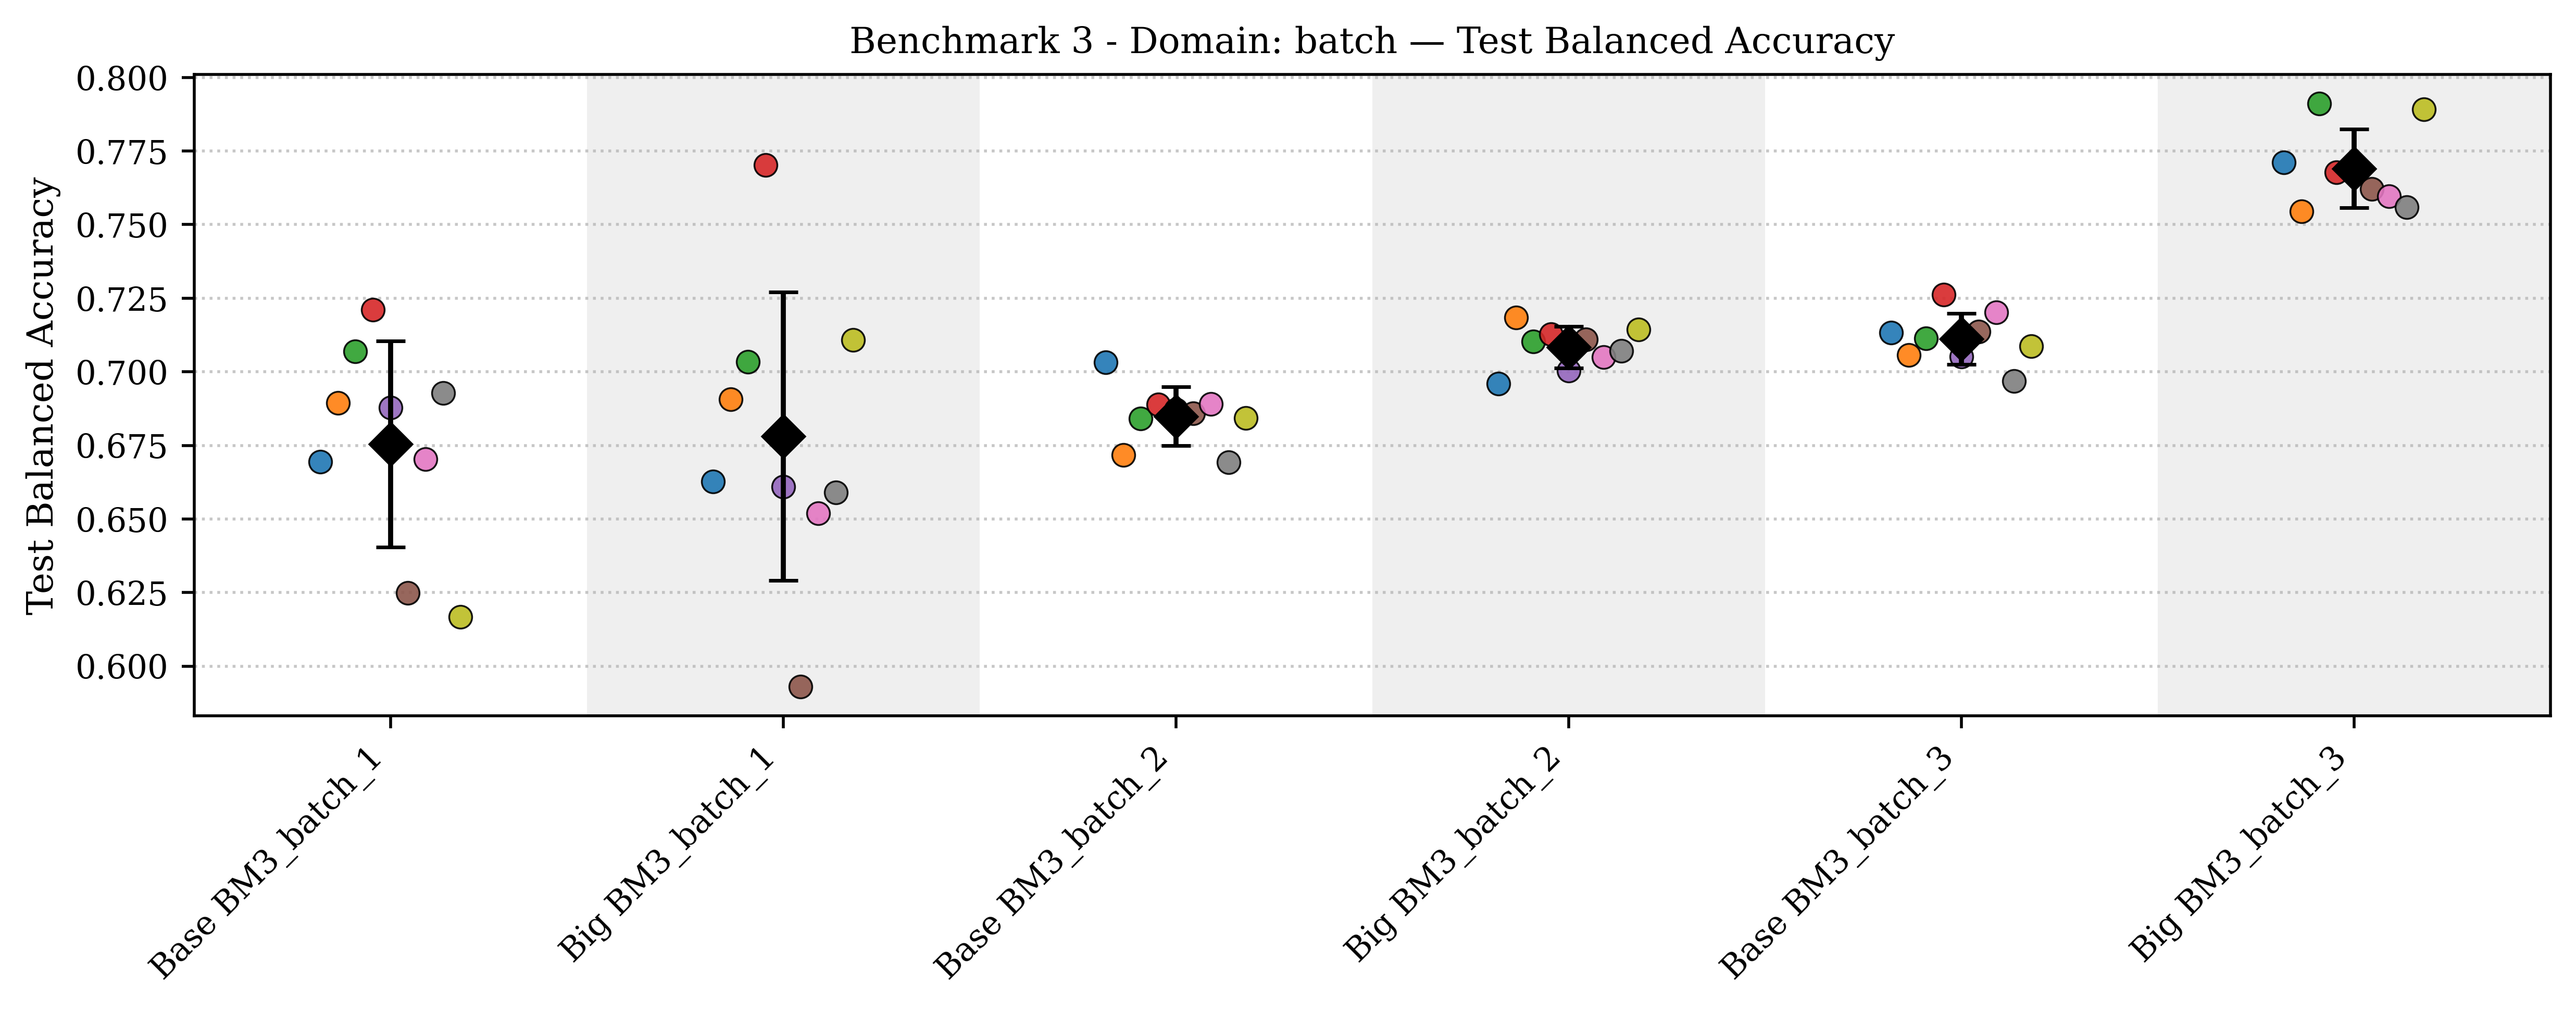
\includegraphics[width=1.0\linewidth]{chapters/7-results/bm3/bm3_batch_test_bal_acc.png}
    \caption{Test balanced accuracy of all of all hole domains specified in \tabref{tab:bm2_domains} evaluated on both the Base and Big config.}
    \label{fig:bm3_batch_test_bal_acc}
\end{figure}

\begin{figure}[htbp]
    \centering
    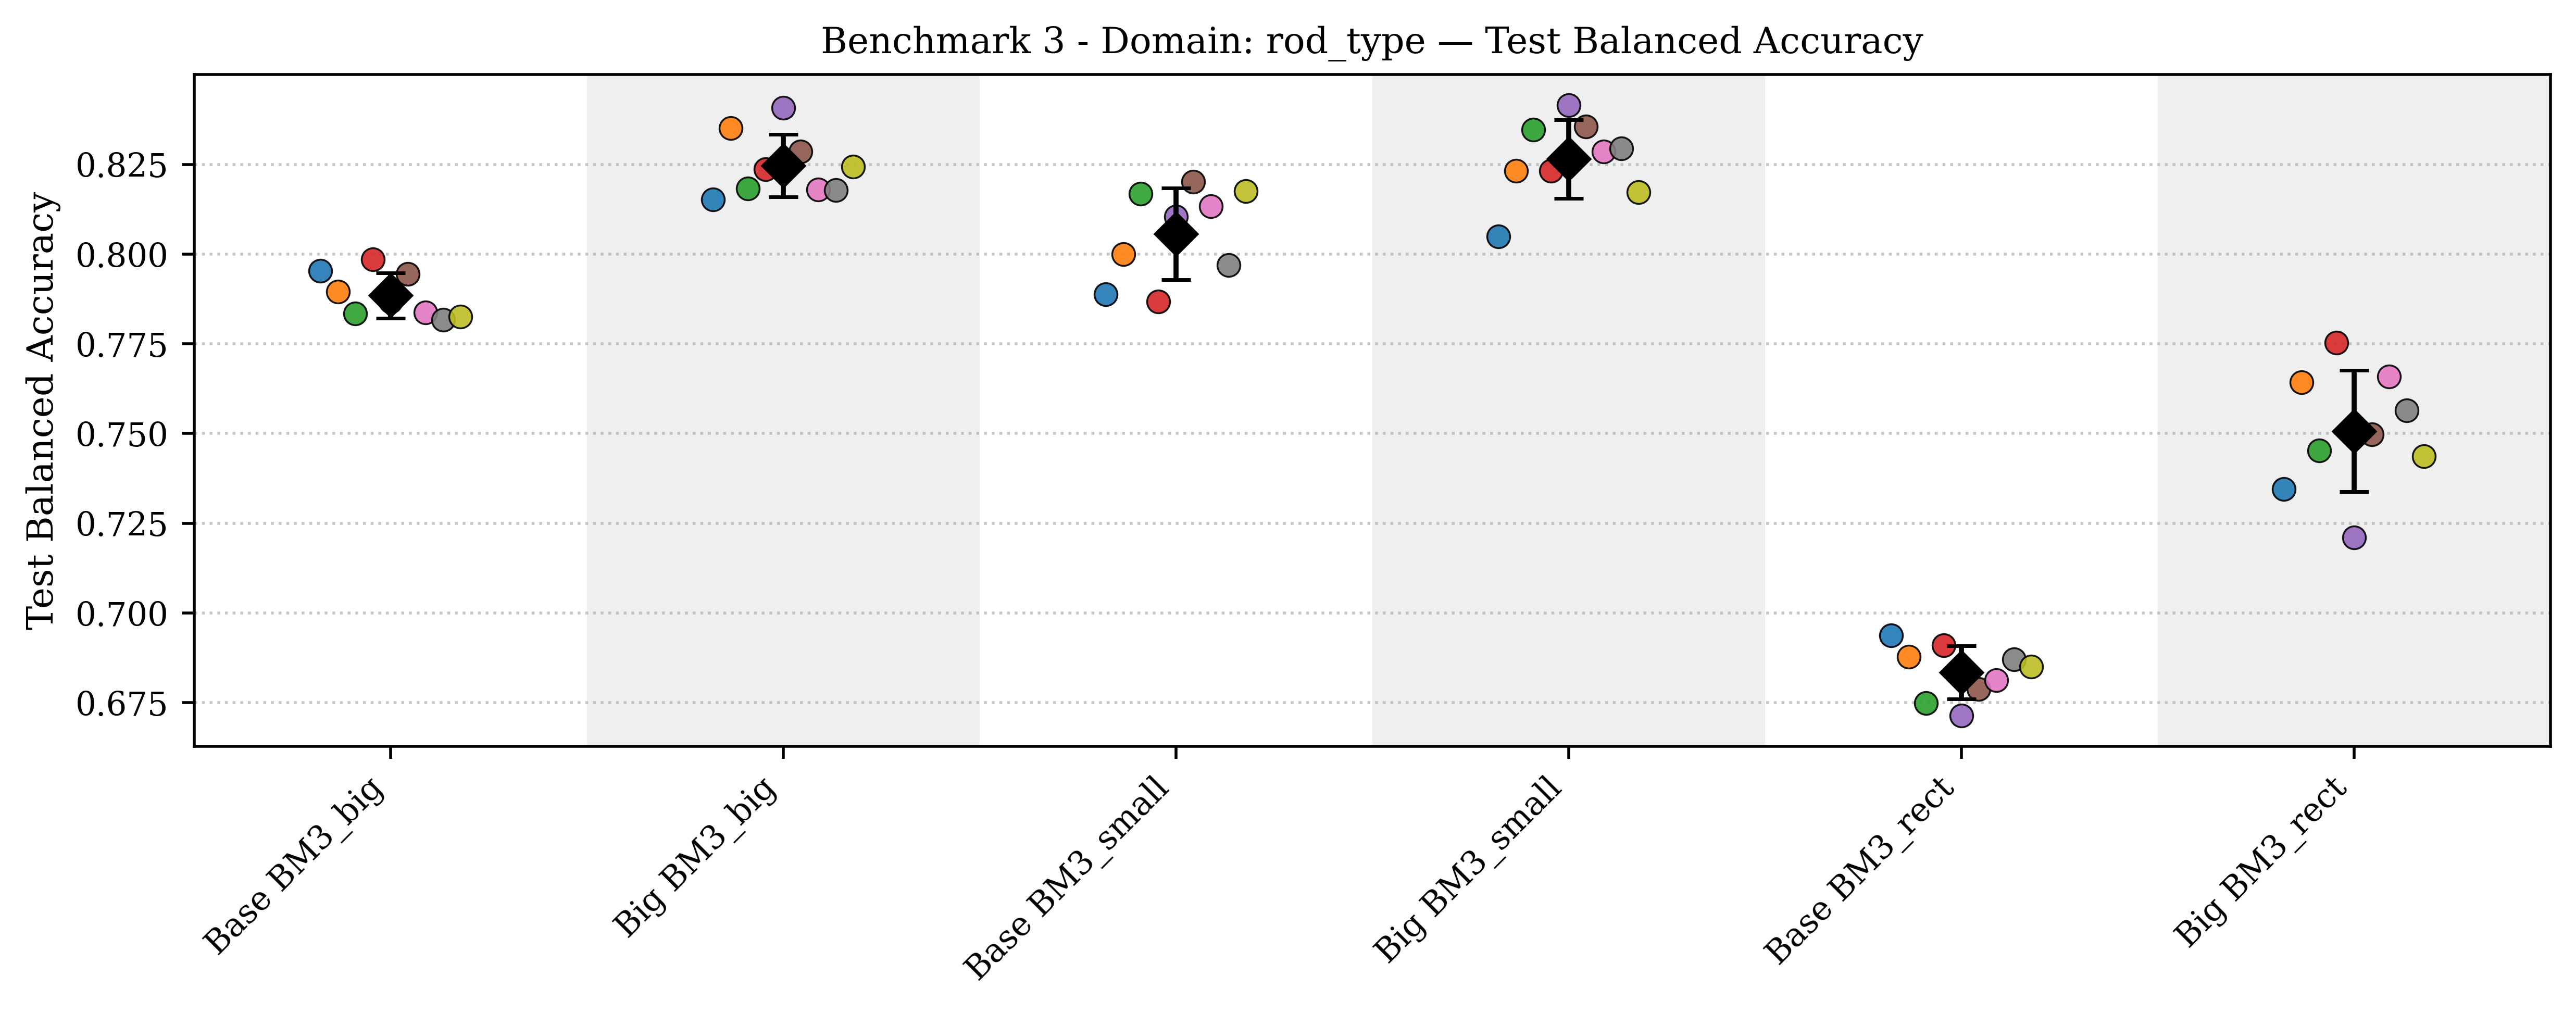
\includegraphics[width=1.0\linewidth]{chapters/7-results/bm3/bm3_rod_type_test_bal_acc.png}
    \caption{Test balanced accuracy of all of all hole domains specified in \tabref{tab:bm2_domains} evaluated on both the Base and Big config.}
    \label{fig:bm3_rod_type_test_bal_acc}
\end{figure}

\begin{figure}[htbp]
    \centering
    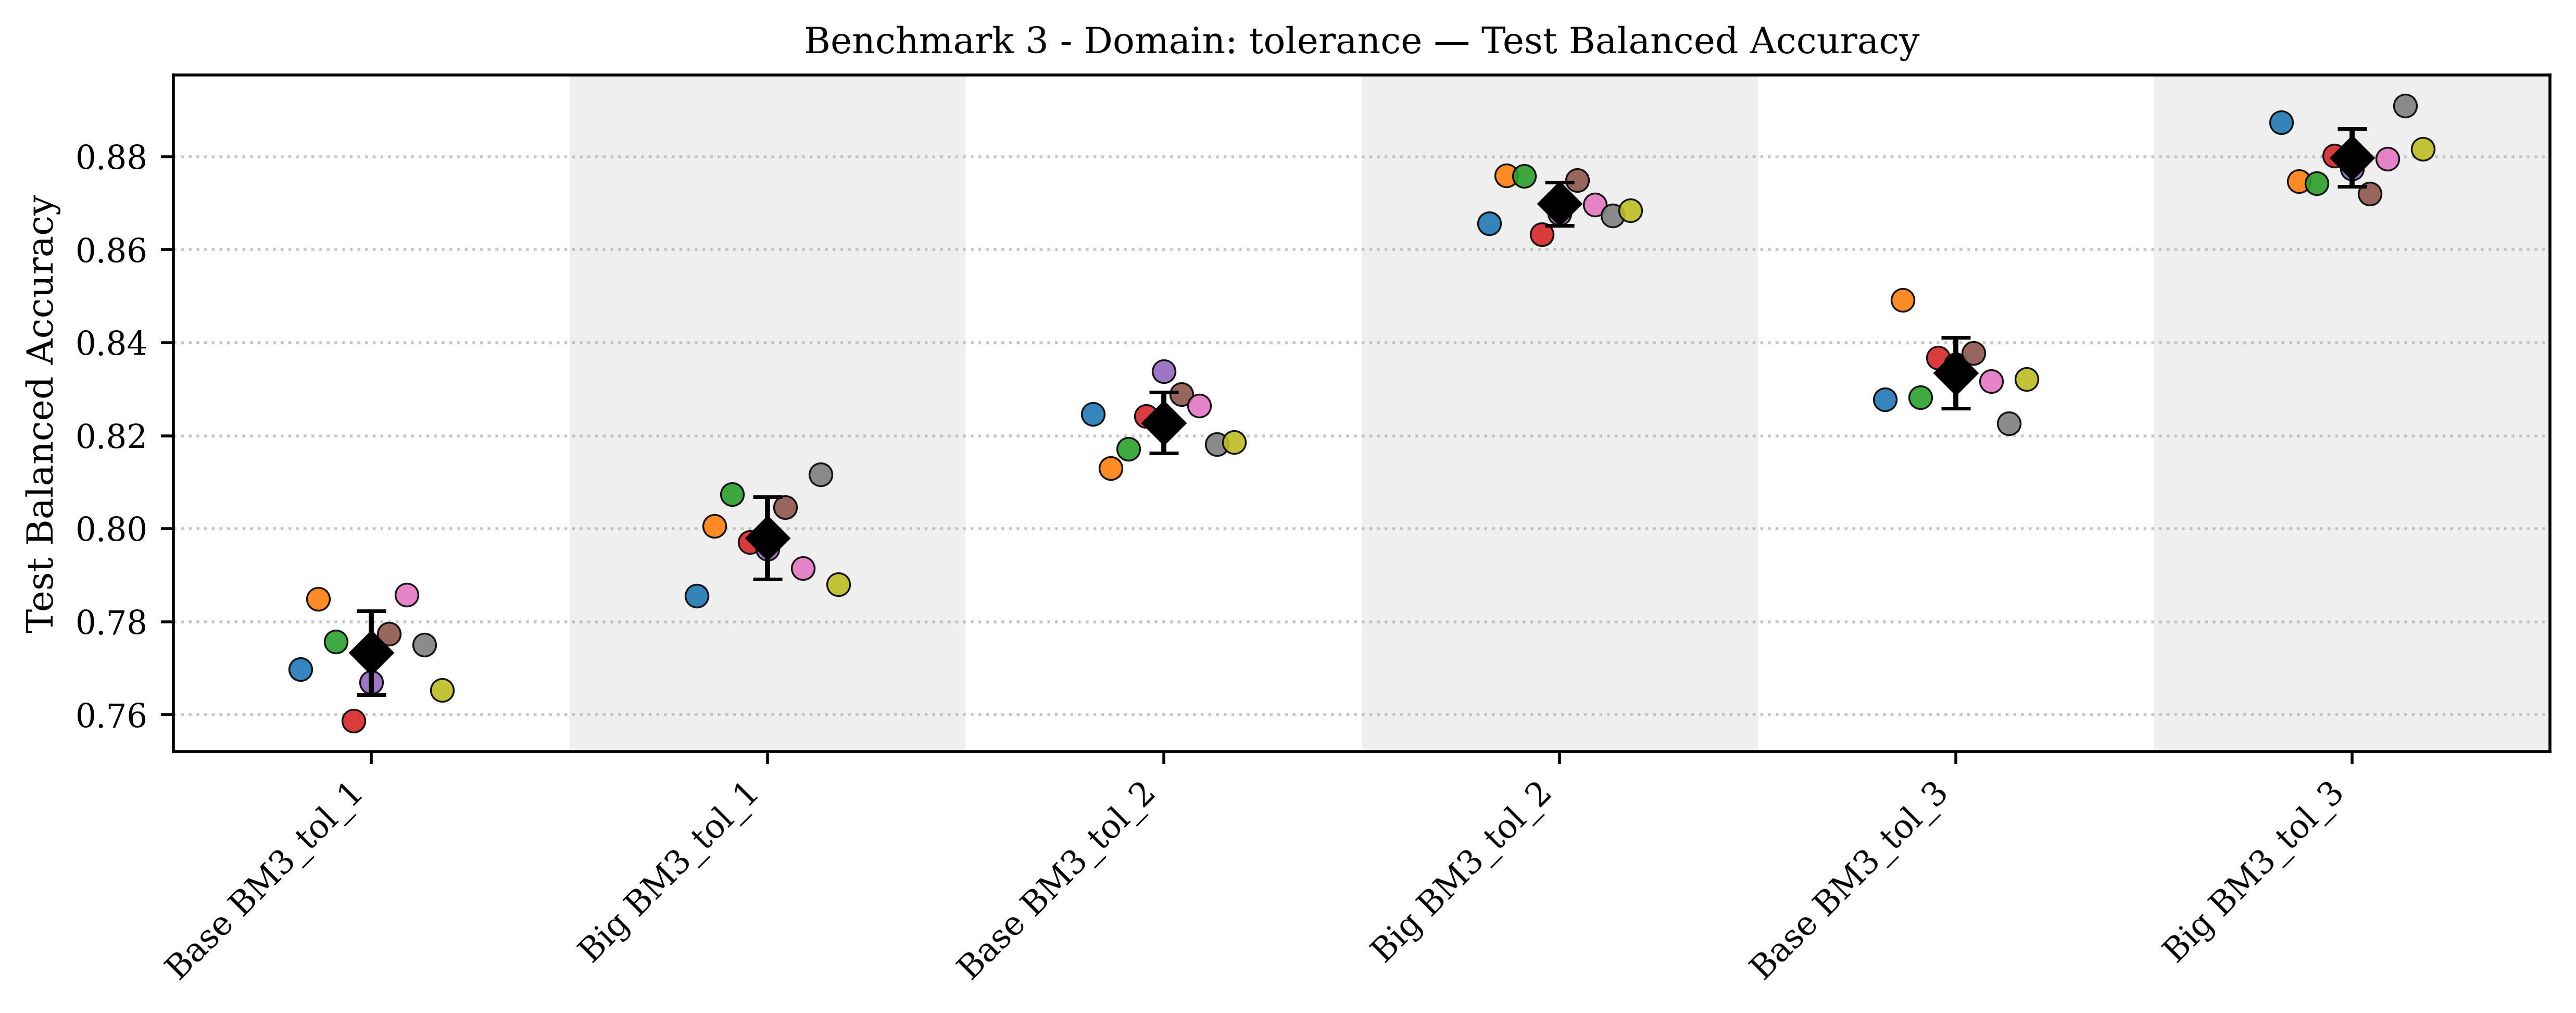
\includegraphics[width=1.0\linewidth]{chapters/7-results/bm3/bm3_tolerance_test_bal_acc.png}
    \caption{Test balanced accuracy of all of all hole domains specified in \tabref{tab:bm2_domains} evaluated on both the Base and Big config.}
    \label{fig:bm3_tolerance_test_bal_acc}
\end{figure}

\begin{figure}[htbp]
    \centering
    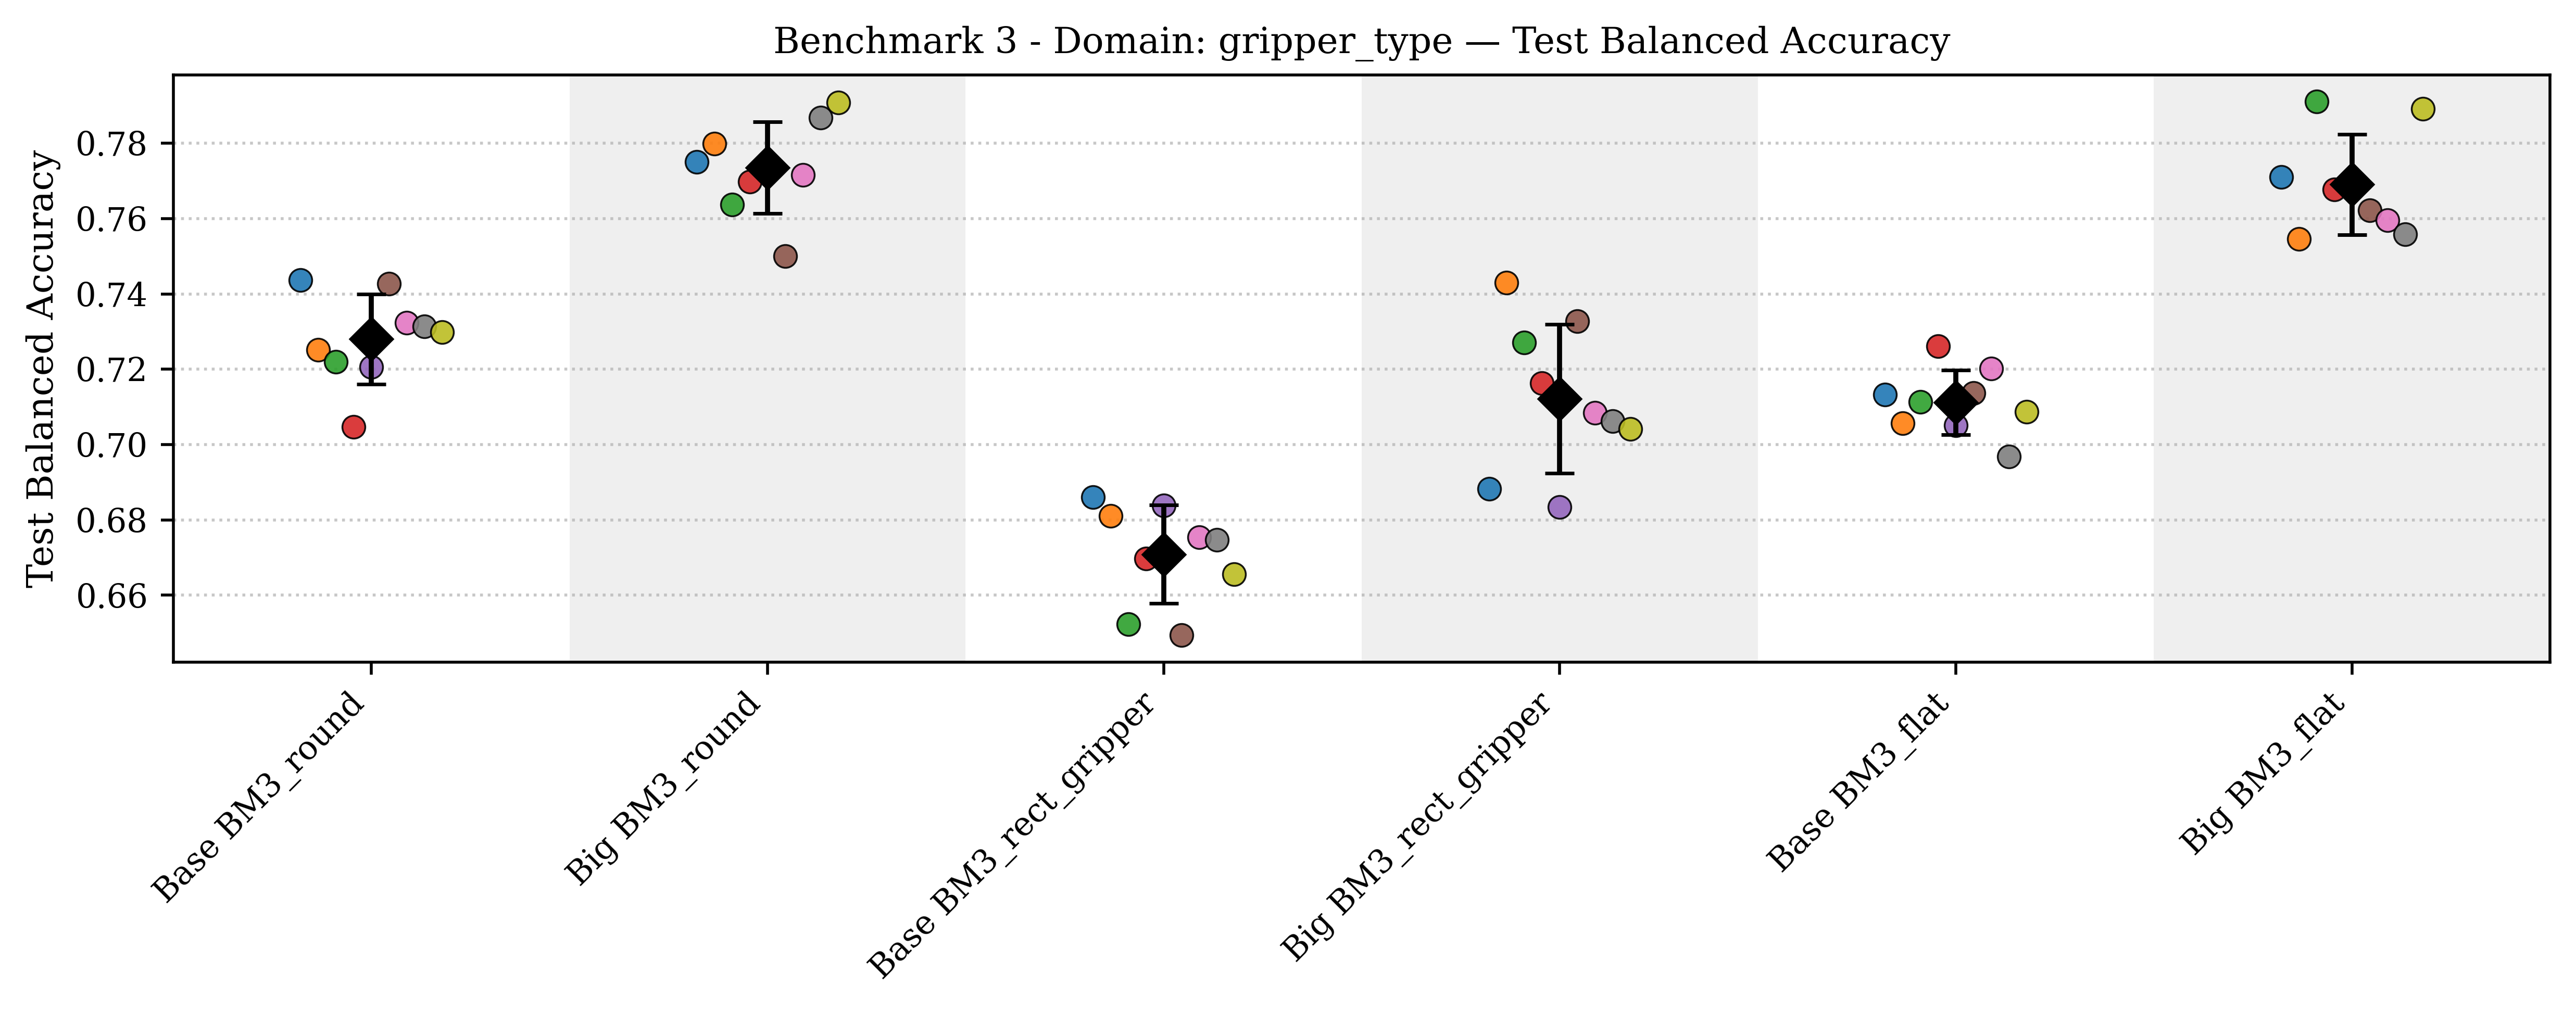
\includegraphics[width=1.0\linewidth]{chapters/7-results/bm3/bm3_gripper_type_test_bal_acc.png}
    \caption{Test balanced accuracy of all of all hole domains specified in \tabref{tab:bm2_domains} evaluated on both the Base and Big config.}
    \label{fig:bm3_gripper_type_test_bal_acc}
\end{figure}

\begin{figure}[htbp]
    \centering
    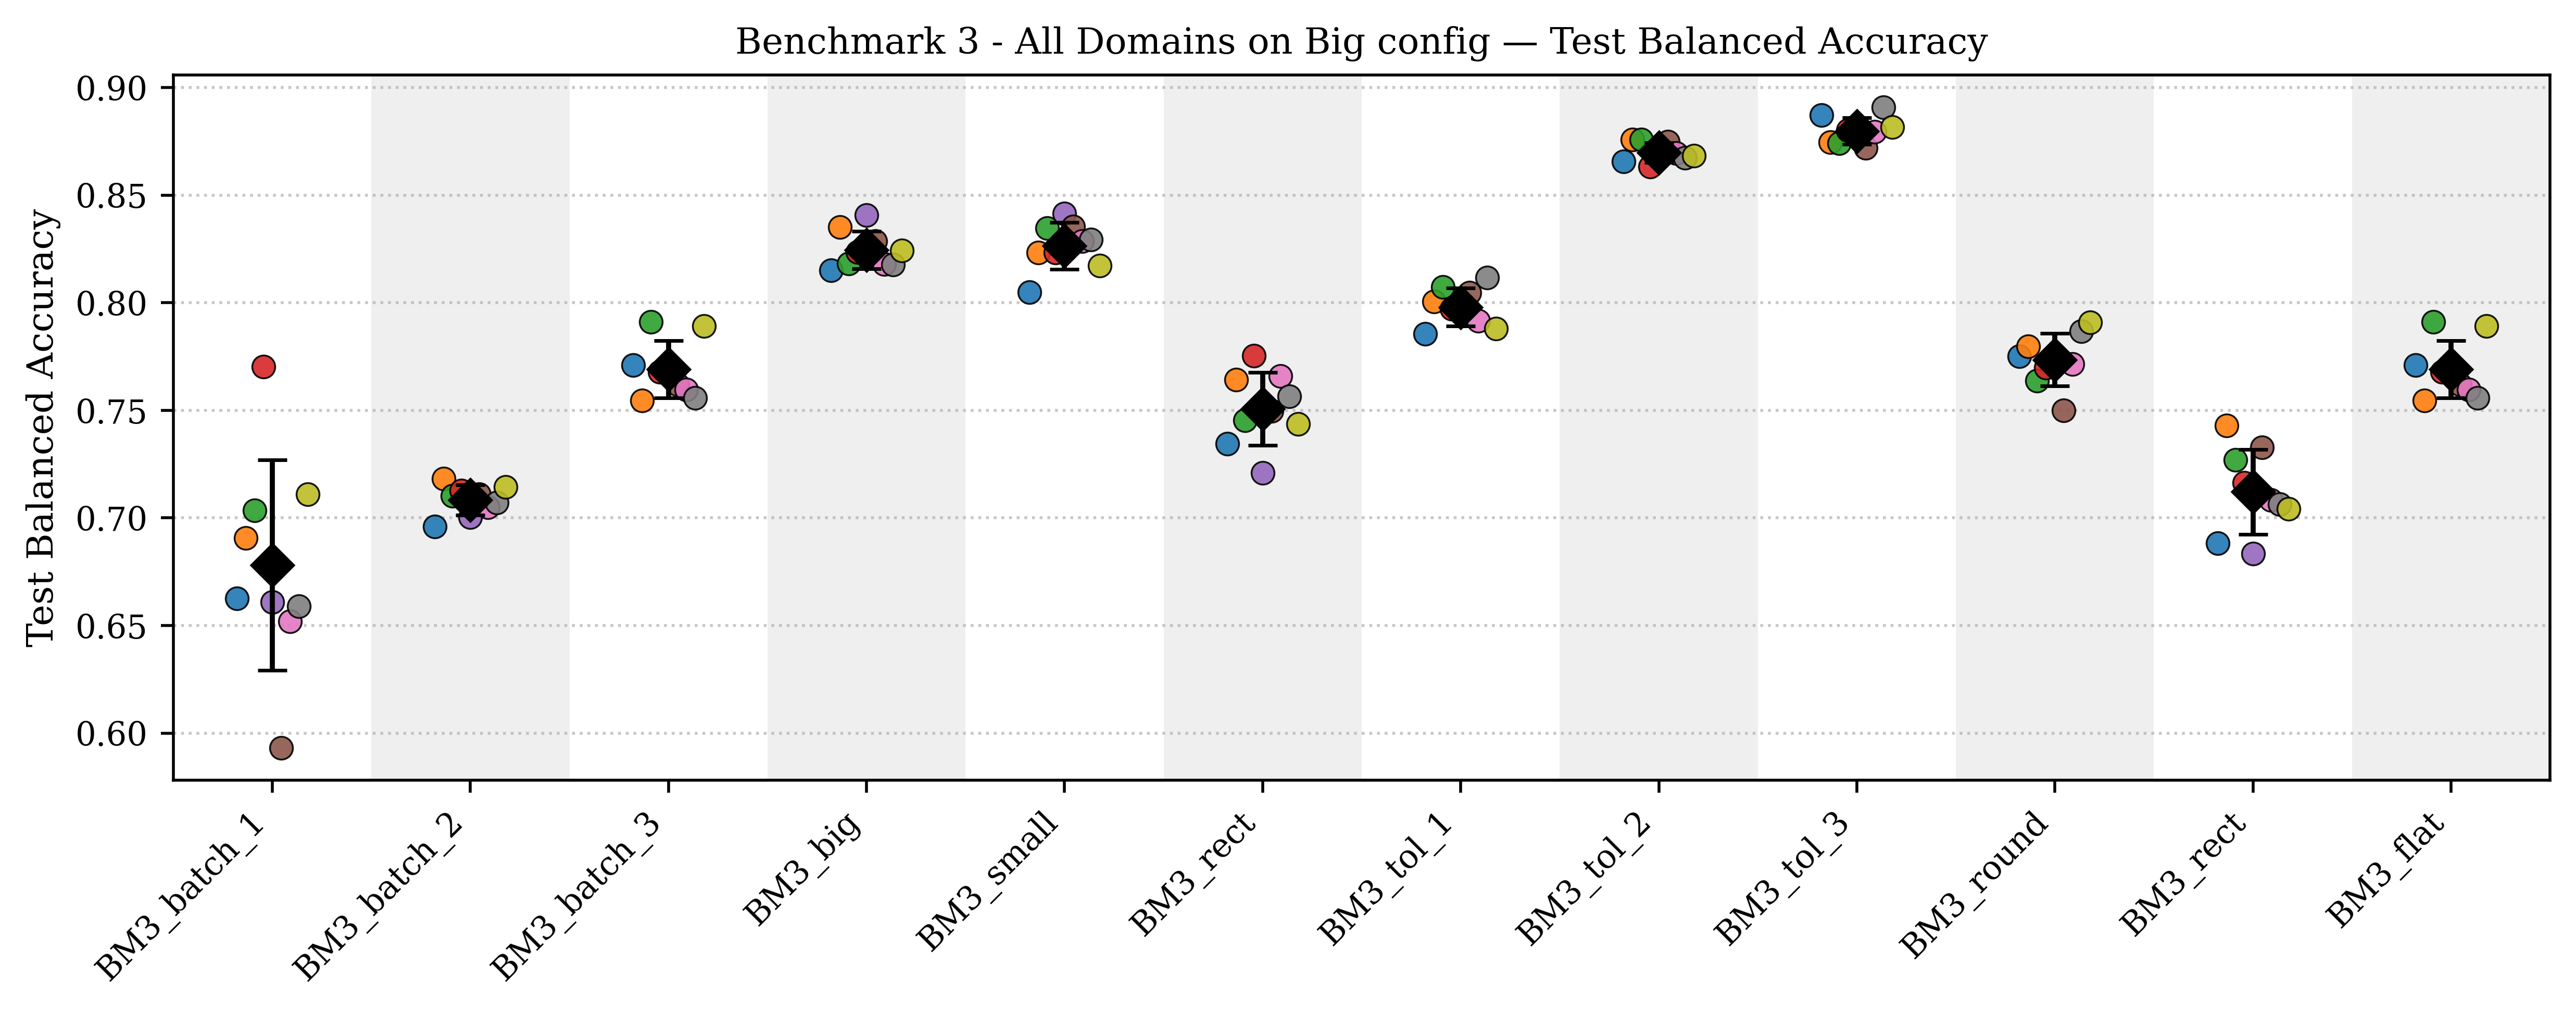
\includegraphics[width=1.0\linewidth]{chapters/7-results/bm3/bm3_all_domains_test_bal_acc.png}
    \caption{Test balanced accuracy of all of all hole domains specified in \tabref{tab:bm2_domains} evaluated on both the Base and Big config.}
    \label{fig:bm3_all_domains_test_bal_acc}
\end{figure}

\begin{table}[htbp]
    \centering
    \caption{Test balanced accuracy detailed results of Benchmark 3.}
    \label{tab:bm3_bal_acc_detail}
    \begin{tabular}{llll}
        \toprule
        \textbf{Domain} & \textbf{Mean $\pm$ std} & \textbf{Min (ms, ss)} & \textbf{Max (ms, ss)}\\
        \midrule

        \texttt{Base BM3\_batch\_1} & \underline{0.6754} $\pm$ \underline{0.0350} & \underline{0.6168 (420, 420)} & \underline{0.7211 (69, 42)}\\
        \texttt{Big BM3\_batch\_1} & 0.6781 $\pm$ 0.0490 & 0.5930 (69, 420) & 0.7703 (69, 42) \\
        \texttt{Base BM3\_batch\_2} & 0.6848 $\pm$ 0.0100 & 0.6692 (420, 69) & 0.7033 (42, 42)\\
        \texttt{Big BM3\_batch\_2} & 0.7083 $\pm$ 0.0070 & 0.6959 (42, 42) & 0.7183 (42, 69) \\
        \texttt{Base BM3\_batch\_3} & 0.7112 $\pm$ 0.0086 & 0.6968 (420, 69) & 0.7261 (69, 42)\\
        \texttt{Big BM3\_batch\_3} & \textbf{0.7691} $\pm$ \textbf{0.0133} & \textbf{0.7545 (42, 69)} & \textbf{0.7911 (42, 420)} \\
        \midrule
        \texttt{Base BM3\_big} & 0.7884 $\pm$ 0.0062 & 0.7817 (420, 69) & 0.7985 (69, 42)\\
        \texttt{Big BM3\_big} & 0.8246 $\pm$ 0.0087 & 0.8151 (42, 42) & 0.8407 (69, 69) \\
        \texttt{Base BM3\_small} & 0.8056 $\pm$ 0.0128 & 0.7867 (69, 42) & 0.8202 (69, 420)\\
        \texttt{Big BM3\_small} & \textbf{0.8265} $\pm$ \textbf{0.0109} & \textbf{0.8049 (42, 42)} & \textbf{0.8415 (69, 69)} \\
        \texttt{Base BM3\_rect} & \underline{0.6834} $\pm$ \underline{0.0074} & \underline{0.6714 (69, 69)} & \underline{0.6937 (42, 42)}\\
        \texttt{Big BM3\_rect} & 0.7507 $\pm$ 0.0169 & 0.7210 (69, 69) & 0.7753 (69, 42) \\
        \midrule
        \texttt{Base BM3\_tol\_1} & \underline{0.7733} $\pm$ \underline{0.0090} & \underline{0.7587 (69, 42)} & \underline{0.7858 (420, 42)}\\
        \texttt{Big BM3\_tol\_1} & 0.7980 $\pm$ 0.0088 & 0.7856 (42, 42) & 0.8116 (420, 69) \\
        \texttt{Base BM3\_tol\_2} & 0.8228 $\pm$ 0.0065 & 0.8130 (42, 69) & 0.8338 (69, 69)\\
        \texttt{Big BM3\_tol\_2} & 0.8698 $\pm$ 0.0046 & 0.8633 (69, 42) & 0.8759 (42, 69) \\
        \texttt{Base BM3\_tol\_3} & 0.8335 $\pm$ 0.0076 & 0.8227 (420, 69) & 0.8492 (42, 69)\\
        \texttt{Big BM3\_tol\_3} & \textbf{0.8798} $\pm$ \textbf{0.0062} & \textbf{0.8720 (69, 420)} & \textbf{0.8909 (420, 69)} \\
        \midrule
        \texttt{Base BM3\_round} & 0.7280 $\pm$ 0.0119 & 0.7047 (69, 42) & 0.7437 (42, 42)\\
        \texttt{Big BM3\_round} & \textbf{0.7735} $\pm$ \textbf{0.0121} & \textbf{0.7501 (69, 420)} & \textbf{0.7908 (420, 420)} \\
        \texttt{Base BM3\_rect\_gripper} & \underline{0.6709} $\pm$ \underline{0.0131} & \underline{0.6494 (69, 420)} & \underline{0.6861 (42, 42)}\\
        \texttt{Big BM3\_rect\_gripper} & 0.7122 $\pm$ 0.0197 & 0.6833 (69, 69) & 0.7430 (42, 69) \\
        \texttt{Base BM3\_flat} & 0.7112 $\pm$ 0.0086 & 0.6968 (420, 69) & 0.7261 (69, 42)\\
        \texttt{Big BM3\_flat} & 0.7691 $\pm$ 0.0133 & 0.7545 (42, 69) & 0.7911 (42, 420) \\
        \bottomrule
    \end{tabular}
\end{table}

\begin{table}[htbp]
    \centering
    \caption{Exact Train, Validation, Test splits with class balance for Benchmark 3.}
    \label{tab:bm3_data_split}
    \begin{tabular}{llll}
        \toprule
        \textbf{Domain} & \textbf{Training (pos, neg)} & \textbf{Validation (pos, neg)} & \textbf{Test (pos, neg)}\\
        \midrule

        \texttt{BM3\_batch\_1} & 6120 (3322, 2798) & 1080 (586, 494) & 900 (484, 416) \\
        \texttt{BM3\_batch\_2} & 3825 (2054, 1771) & 675 (362, 313) & 3600 (1976, 1624) \\
        \texttt{BM3\_batch\_3} & 3825 (2091, 1734) & 675 (369, 306) & 3600 (1932, 1668) \\

        \texttt{BM3\_big} & 4590 (2502, 2088) & 810 (442, 368) & 2700 (1448, 1252) \\
        \texttt{BM3\_small} & 4590 (2427, 2163) & 810 (428, 382) & 2700 (1537, 1163) \\
        \texttt{BM3\_rect} & 4590 (2537, 2053) & 810 (448, 362) & 2700 (1407, 1293) \\

        \texttt{BM3\_tol\_1} & 4182 (2277, 1905) & 738 (402, 336) & 3180 (1713, 1467) \\
        \texttt{BM3\_tol\_2} & 4794 (2523, 2271) & 846 (445, 401) & 2460 (1424, 1036) \\
        \texttt{BM3\_tol\_3} & 4794 (2666, 2128) & 846 (471, 375) & 2460 (1255, 1205) \\

        \texttt{BM3\_round} & 4335 (2313, 2022) & 765 (408, 357) & 3000 (1671, 1329) \\
        \texttt{BM3\_rect} & 5610 (3063, 2547) & 990 (540, 450) & 1500 (789, 711) \\
        \texttt{BM3\_flat} & 3825 (2091, 1734) & 675 (369, 306) & 3600 (1932, 1668) \\
        \bottomrule
    \end{tabular}
\end{table}

\section{Deviation Analysis I: Physical Success Rate}
\label{subsec:results_deviation_analysis_1}

The first part of Deviation Analysis I evaluates the physical success rate across the complete dataset. This corresponds to the domain selection in which all domain attributes are set to \texttt{None}, meaning the whole dataset is selected. The purpose of doing a global investigation first, is to identify deviation groups that show consistent trends or systematic differences in success rate. These isolated deviation groups are then taken further to a more detailed domain-specific analysis in the next Subsection \ref{subsec:da1_domain_investigation}.

\subsection{Global Investigation Across the Full Dataset}
\label{subsec:da1_global_screening}

\figref{fig:da1_physical_position_tilt_global} shows the physical success rate for the individual position-offset and tilt levels. The position-offset groups alone show only low variation, with success rates between 0.52 and 0.58. In contrast, the tilt groups show a noticeable trend. Insertions without relevant tilt reach a success rate of 0.81, while moderate tilt reduces the success rate to 0.62 and large tilt further reduces it to 0.47. This indicates that angular misalignment is a more informative deviation parameter than the radial position offset alone.

The combined position--tilt groups in \figref{fig:da1_physical_position_over_tilt_global} support this interpretation. For each position-offset level, the success rate decreases as the tilt magnitude increases. No-offset insertions decrease from 0.89 for no tilt to 0.47 for large tilt, moderate-offset insertions decrease from 0.87 to 0.45, and large-offset insertions decrease from 0.68 to 0.48. The position offset therefore does not explain the success rate independently of tilt. Instead, the tilt magnitude appears to be the dominant factor in the global dataset, while the effect of position offset becomes more relevant when considered together with tilt.

The offset-direction groups in \figref{fig:da1_physical_offset_direction_global} show a smaller but still visible directional asymmetry. The positive $x$ direction has the highest success rate at 0.61, while the negative $x$ direction has the lowest success rate at 0.48. The $y$ directions lie between these values. This suggests that the insertion process may contain a setup-specific directional bias.
% However, because the differences are smaller than for the tilt groups, the direction effect is mainly treated as a secondary candidate for further investigation.

The force-related groups show a stronger effect. \figref{fig:da1_physical_force_level_and_limit_global} shows that the success rate generally decreases for high commanded force levels, especially for \texttt{F35} and \texttt{F40}. The force limit alone is less directly interpretable, because its effect depends on the force level. This becomes clear in \figref{fig:da1_physical_force_interaction_global}, where the combination of force level and force limit produces large differences in success rate. In particular, combinations where the difference between force level and force limit ($L - F$ in \figref{fig:da1_physical_force_interaction_global}) is close to zero or negative show very low success rates. Therefore, the force interaction is more informative than force level or force limit considered separately.

To further investigate the force interaction, two subsets are shown in \figref{fig:da1_physical_force_no_tilt_no_offset} and \figref{fig:da1_physical_position_tilt_f40_l30}. The first subset in \figref{fig:da1_physical_force_no_tilt_no_offset} considers only insertions without relevant position offset and without relevant tilt. Due to limitations of the deviation planner explained in Section \ref{sec:dataset_collection}, the force limits \texttt{L30} and \texttt{L50} were not recorded with no tilt and no offset, which means that all force levels (\texttt{F15 - F40}) had the force limit \texttt{L40} during insertions. In this specific subset,the force interaction levels \texttt{F15 / L40}, \texttt{F20 / L40}, \texttt{F25 / L40}, and \texttt{F30 / L40} reach a physical success rate of 1.0. This indicates that, in the absence of relevant translational and angular misalignment, several force settings are sufficient for reliable insertion. However, the success rate decreases for higher force levels, especially for \texttt{F40}.

The opposite case is shown in \figref{fig:da1_physical_position_tilt_f40_l30}, where the force interaction is fixed to \texttt{F40/L30}, resulting in a force difference of $30 - 40 = -10$N. Across the available position--tilt groups, the physical success rate remains close to zero. This confirms that the low success rate of \texttt{F40/L30} is not caused by a single position--tilt group alone, but is a generally unfavorable force interaction in the recorded dataset. This result supports the interpretation that the force limit is likely exceeded before the insertion can be completed, when the force level is too close to or above the allowed force limit.

The record offset in \figref{fig:da1_physical_record_offset_global} shows a gradual increase in success rate from the early to the late recording windows. This group is reported for completeness, but it is not interpreted as a physical cause of insertion success or failure.

Finally, \figref{fig:da1_physical_grasp_approach_height_global} shows that grasp height and approach height have comparatively low global effects. The grasp height differs slightly between 0 mm and 7 mm, while the three approach-height levels show almost identical success rates.

The sample counts and class balances for all global deviation groups are listed in \tabref{tab:da1_class_split_global}. The table shows that the deviation groups are not equally sized. This is especially visible for the tilt groups, where the large-tilt group contains substantially more samples than the no-tilt group. This imbalance is due to the goal to have balanced class splits for all levels in a deviation group. \figref{fig:da1_sankey_tilt} visualizes this split exemplarily for the tilt groups and shows how the complete dataset is divided into tilt levels and physical insertion outcomes. This principle holds for every deviation group.

Overall, the global screening identifies tilt magnitude and force interaction as the most relevant deviation groups for further investigation. Offset direction is also considered because it indicates a possible directional asymmetry. In contrast, grasp height and approach height show only weak global effects and are therefore not investigated in detail in the following domain-specific analysis.

\begin{figure}[htbp]
    \centering
    \begin{minipage}[t]{0.45\textwidth}
        \centering
        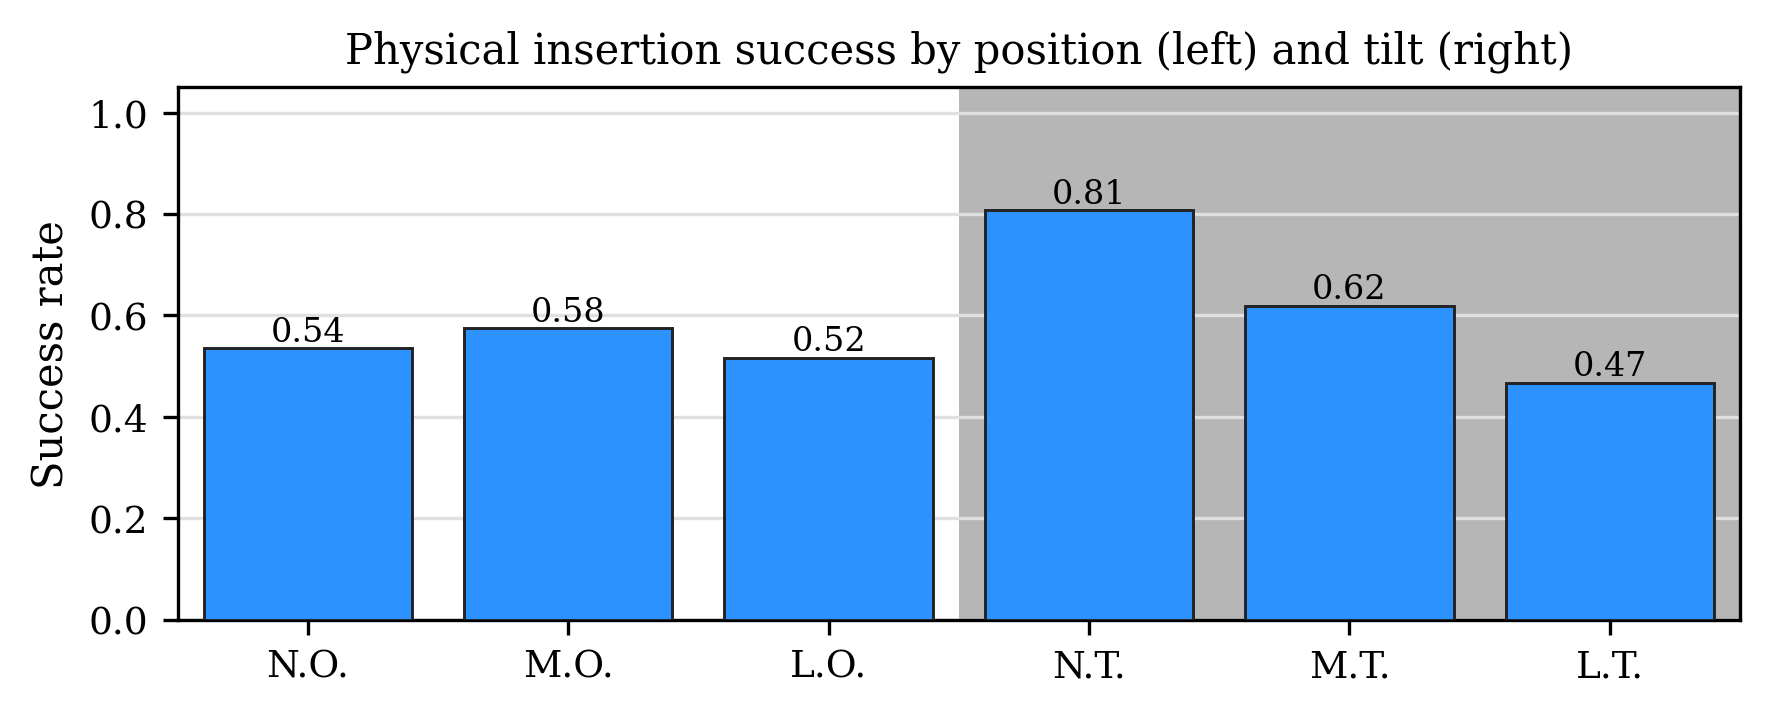
\includegraphics[width=0.95\linewidth]{chapters/7-results/DA1/global/physical_position_and_tilt_global.png}
        \caption{Global physical success rate for position-offset levels and tilt levels.}
        \label{fig:da1_physical_position_tilt_global}
    \end{minipage}
    \hfill
    \begin{minipage}[t]{0.45\textwidth}
        \centering
        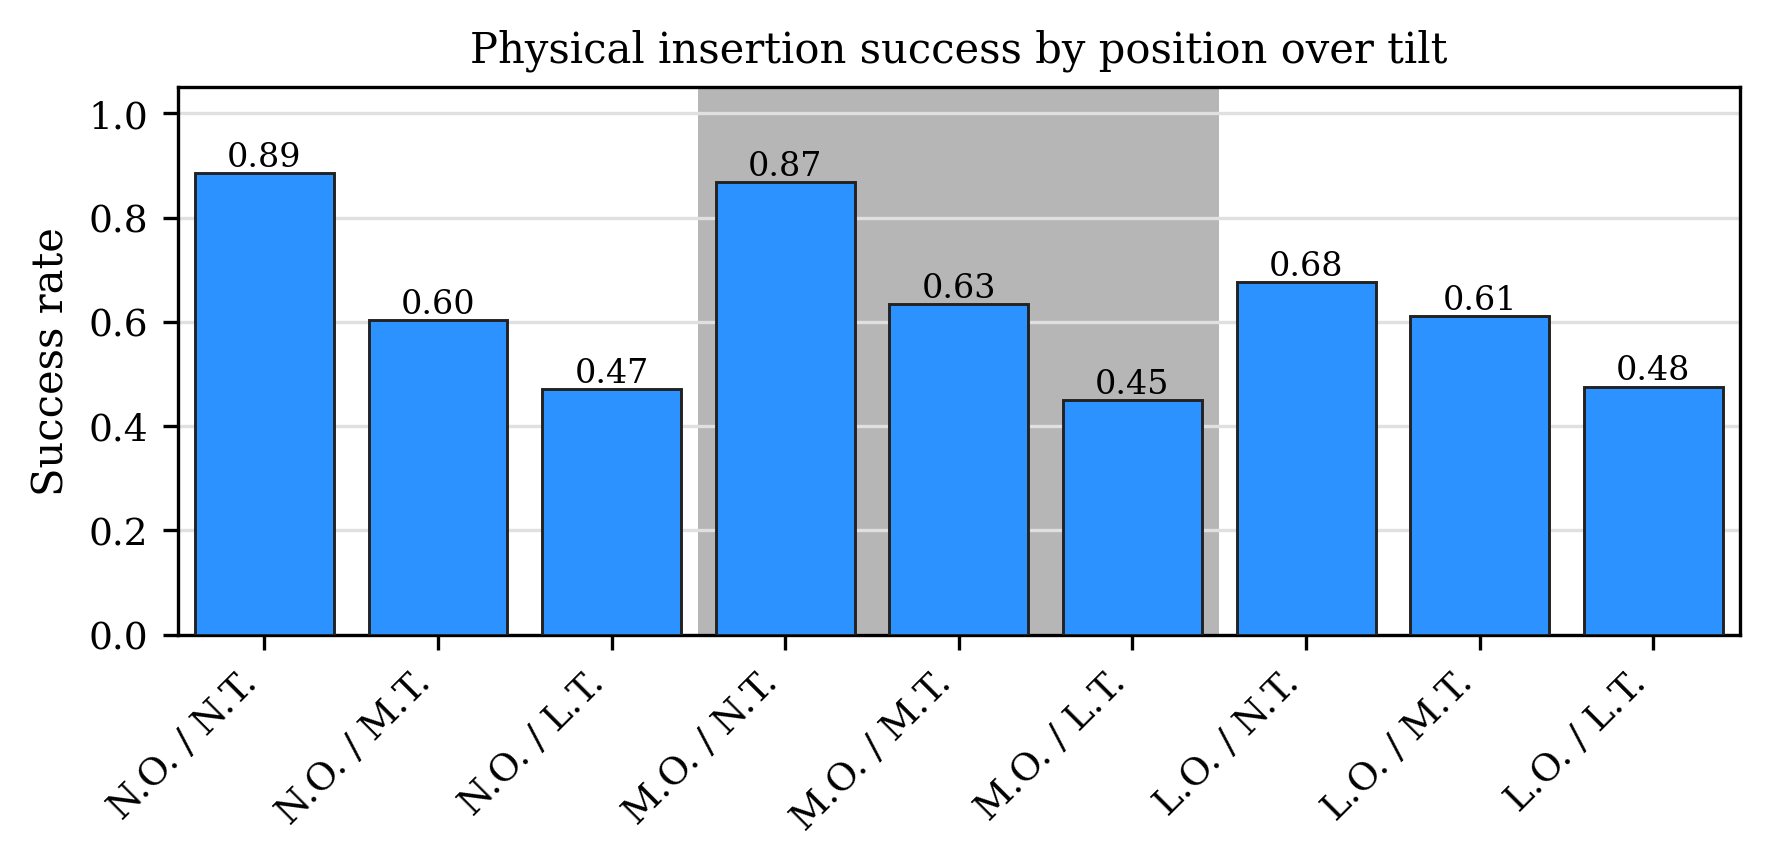
\includegraphics[width=0.95\linewidth]{chapters/7-results/DA1/global/physical_position_over_tilt_global.png}
        \caption{Global physical success rate for combined position--tilt groups.}
        \label{fig:da1_physical_position_over_tilt_global}
    \end{minipage}
\end{figure}


\begin{figure}[htbp]
    \centering
    \begin{minipage}[t]{0.45\textwidth}
        \centering
        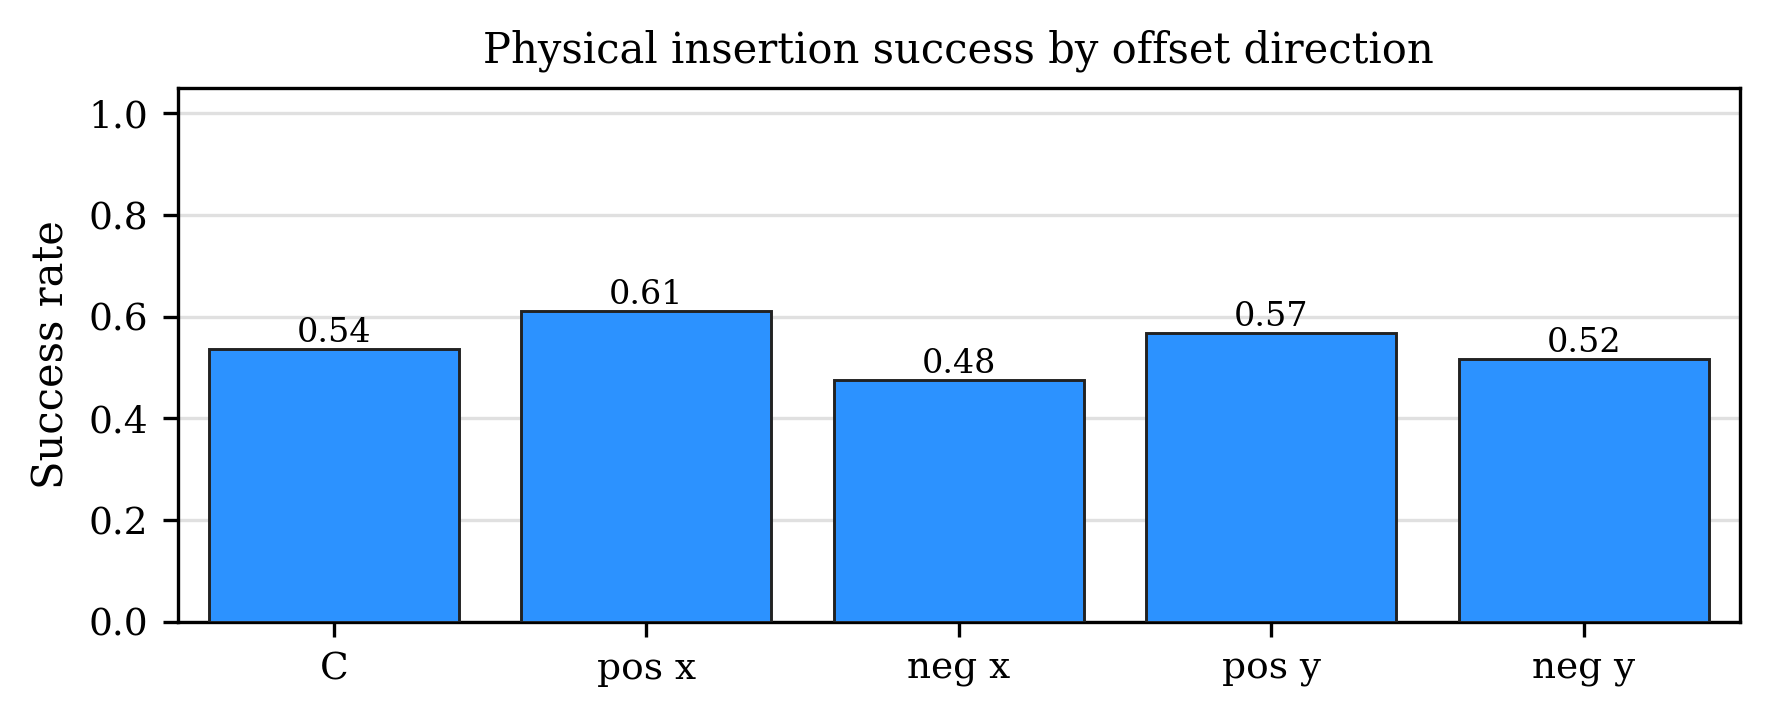
\includegraphics[width=0.9\linewidth]{chapters/7-results/DA1/global/physical_offset_direction_global.png}
        \caption{Global physical success rate for offset-direction groups.}
        \label{fig:da1_physical_offset_direction_global}
    \end{minipage}
    \hfill
    \begin{minipage}[t]{0.45\textwidth}
        \centering
        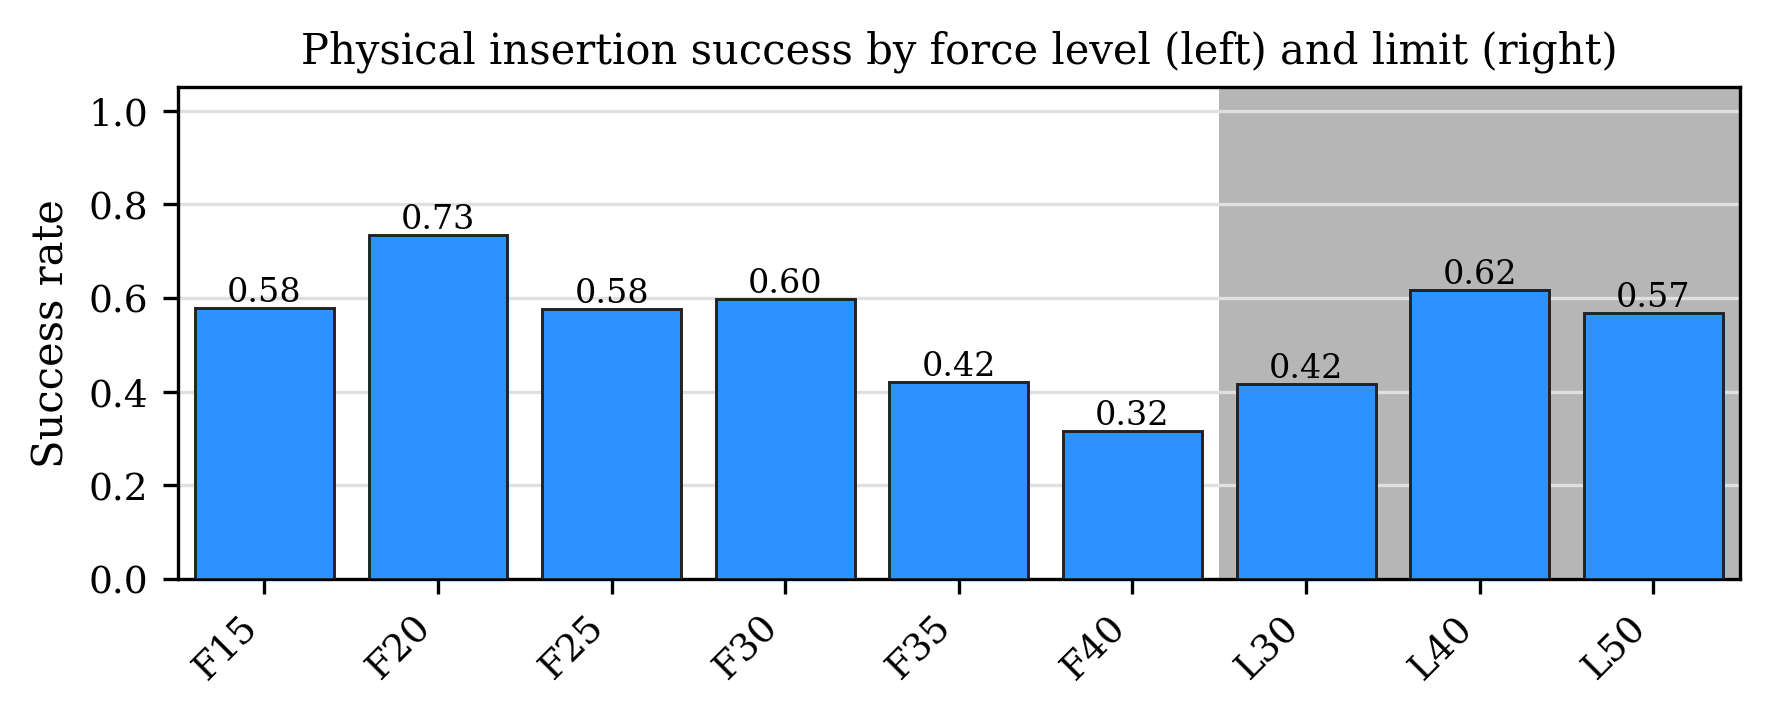
\includegraphics[width=0.9\linewidth]{chapters/7-results/DA1/global/physical_force_level_and_limit_global.png}
        \caption{Global physical success rate for force level and force limit.}
        \label{fig:da1_physical_force_level_and_limit_global}
    \end{minipage}
\end{figure}

\begin{figure}[htbp]
    \centering
    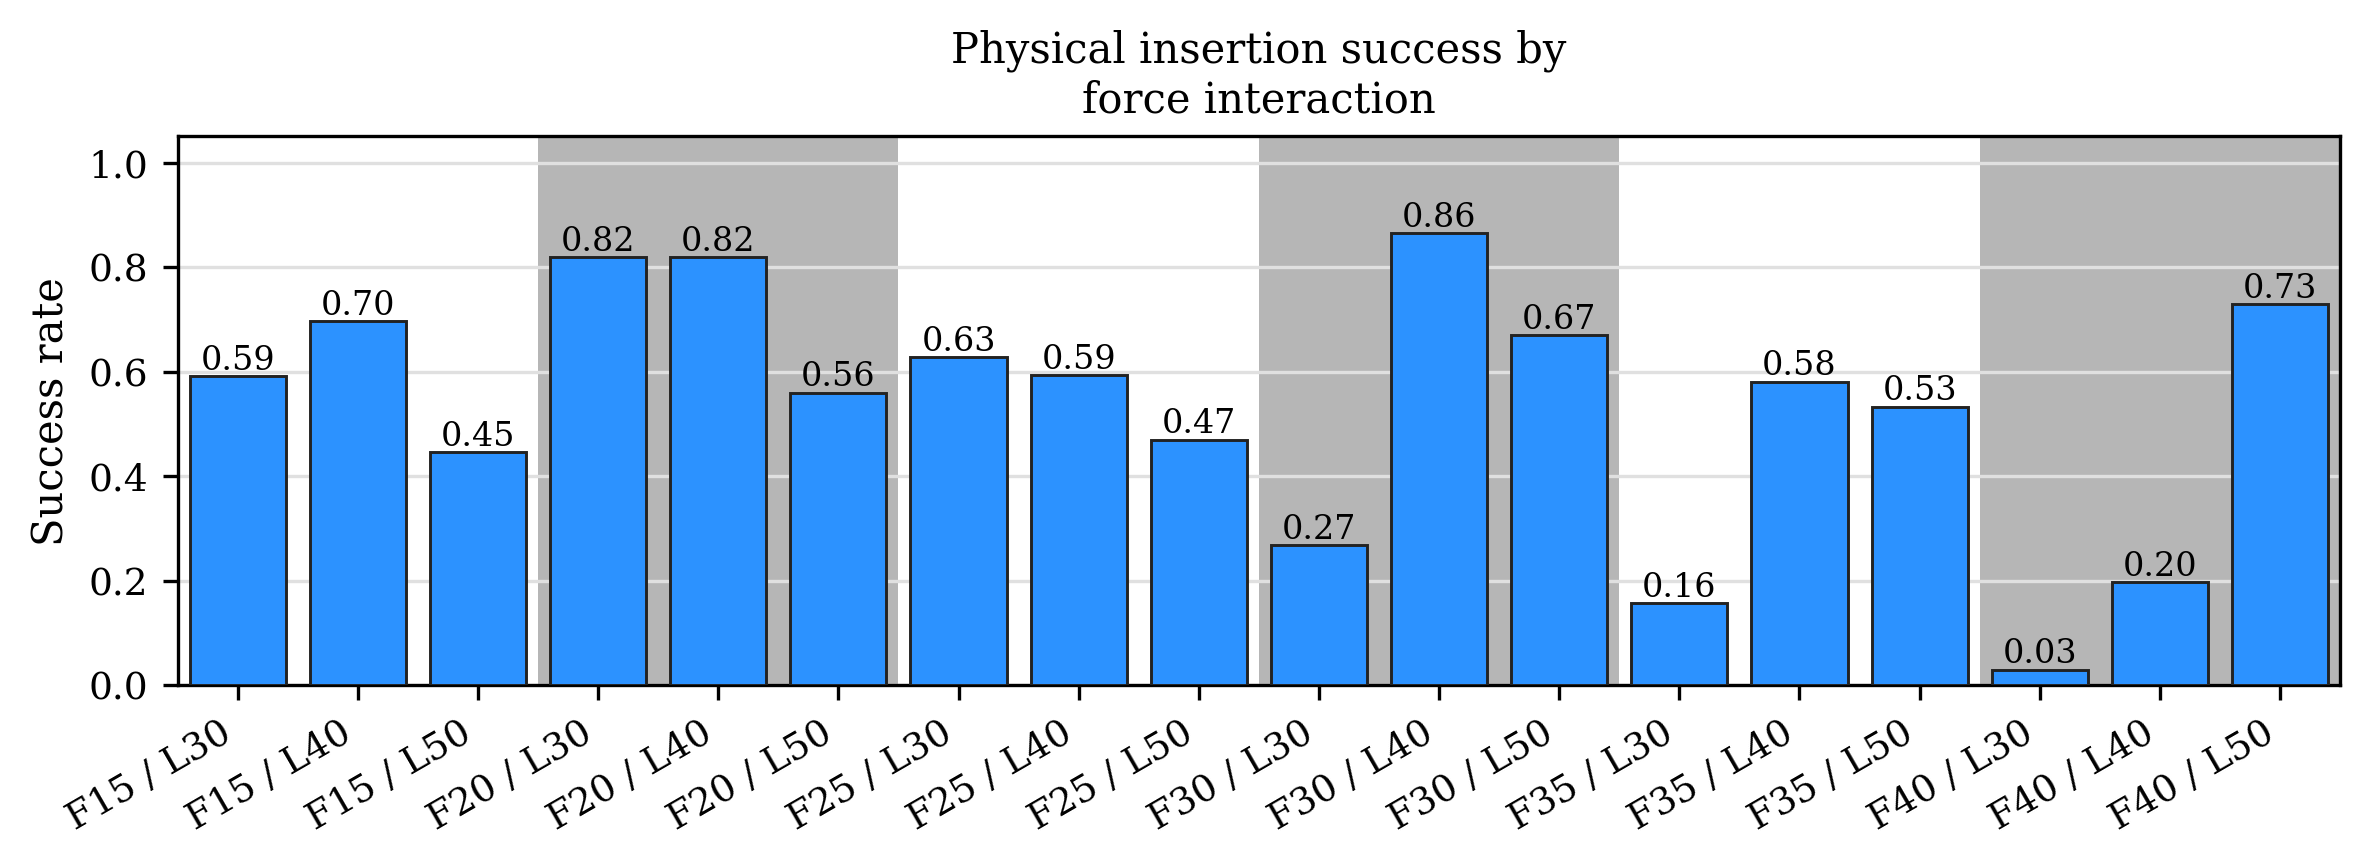
\includegraphics[width=0.9\linewidth]{chapters/7-results/DA1/global/physical_force_interaction_global.png}
    \caption{Global physical success rate for force-interaction groups. The label \texttt{D} denotes the difference between force limit and commanded force level.}
    \label{fig:da1_physical_force_interaction_global}
\end{figure}

\begin{figure}[htbp]
    \centering
    \begin{minipage}[t]{0.49\textwidth}
        \centering
        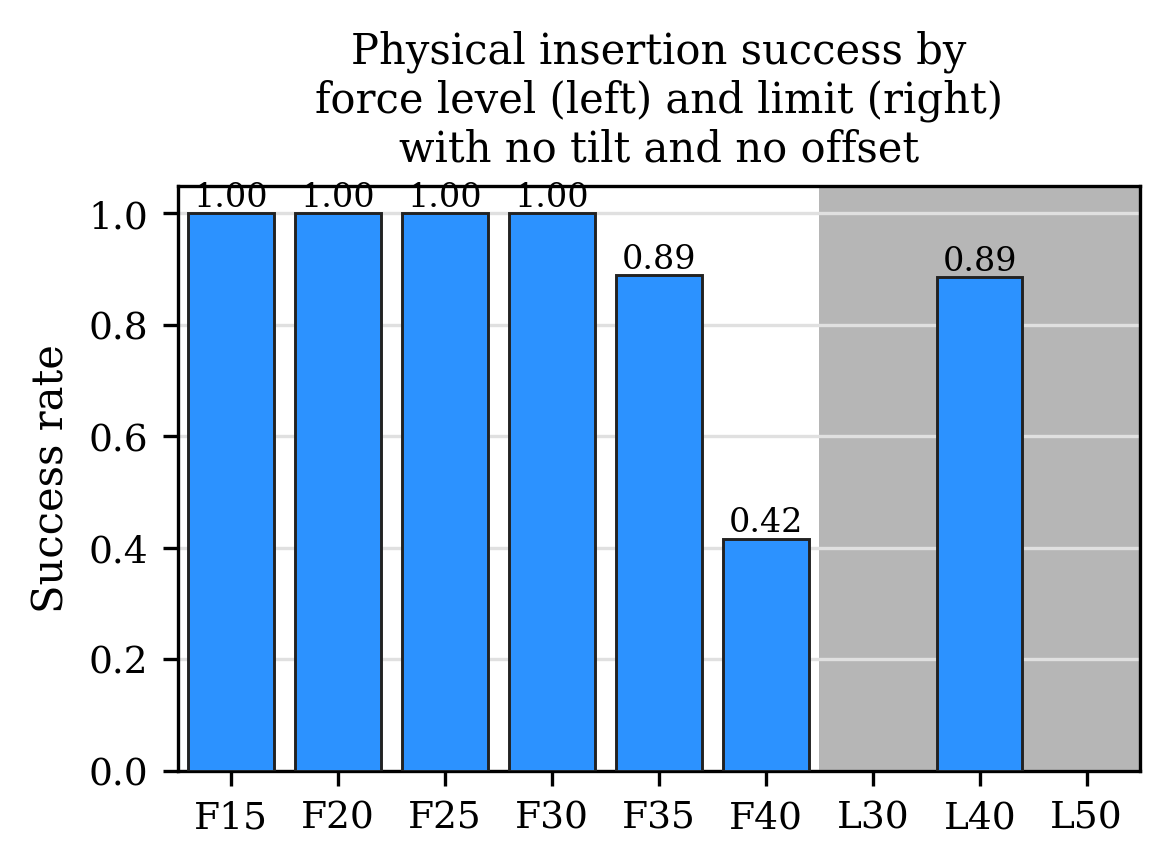
\includegraphics[width=0.99\linewidth]{chapters/7-results/DA1/global/physical_F_L_NT_NO_global.png}
        \caption{Physical success rate for force level and force limit under no tilt and no offset. Missing bars indicate that no samples were available for the corresponding force-limit level in this subset.}
        \label{fig:da1_physical_force_no_tilt_no_offset}
    \end{minipage}
    \hfill
    \begin{minipage}[t]{0.49\textwidth}
        \centering
        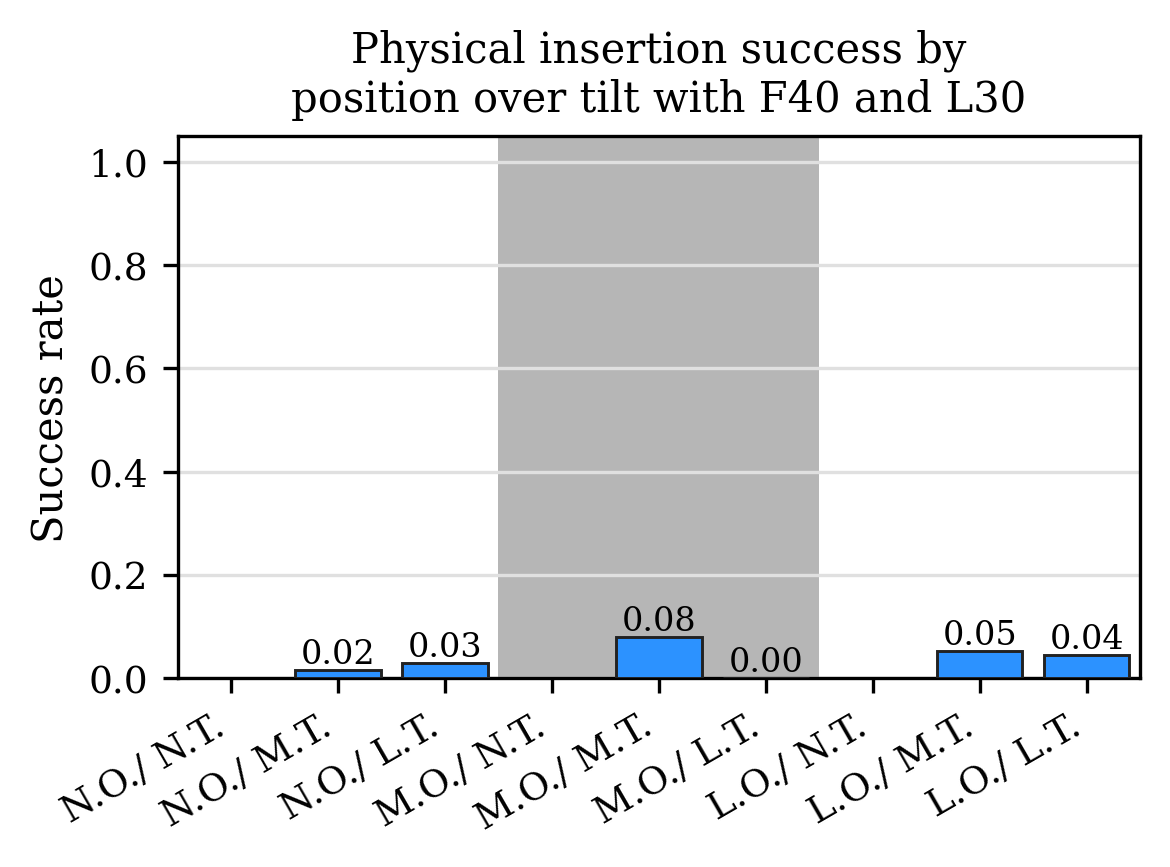
\includegraphics[width=0.99\linewidth]{chapters/7-results/DA1/global/physical_position_over_tilt_F40_L30_global.png}
        \caption{Physical success rate of position--tilt groups for the force interaction \texttt{F40/L30}. Missing bars indicate unavailable deviation combinations in this subset.}
        \label{fig:da1_physical_position_tilt_f40_l30}
    \end{minipage}
\end{figure}

\begin{figure}[htbp]
    \centering
    \begin{minipage}[t]{0.45\textwidth}
        \centering
        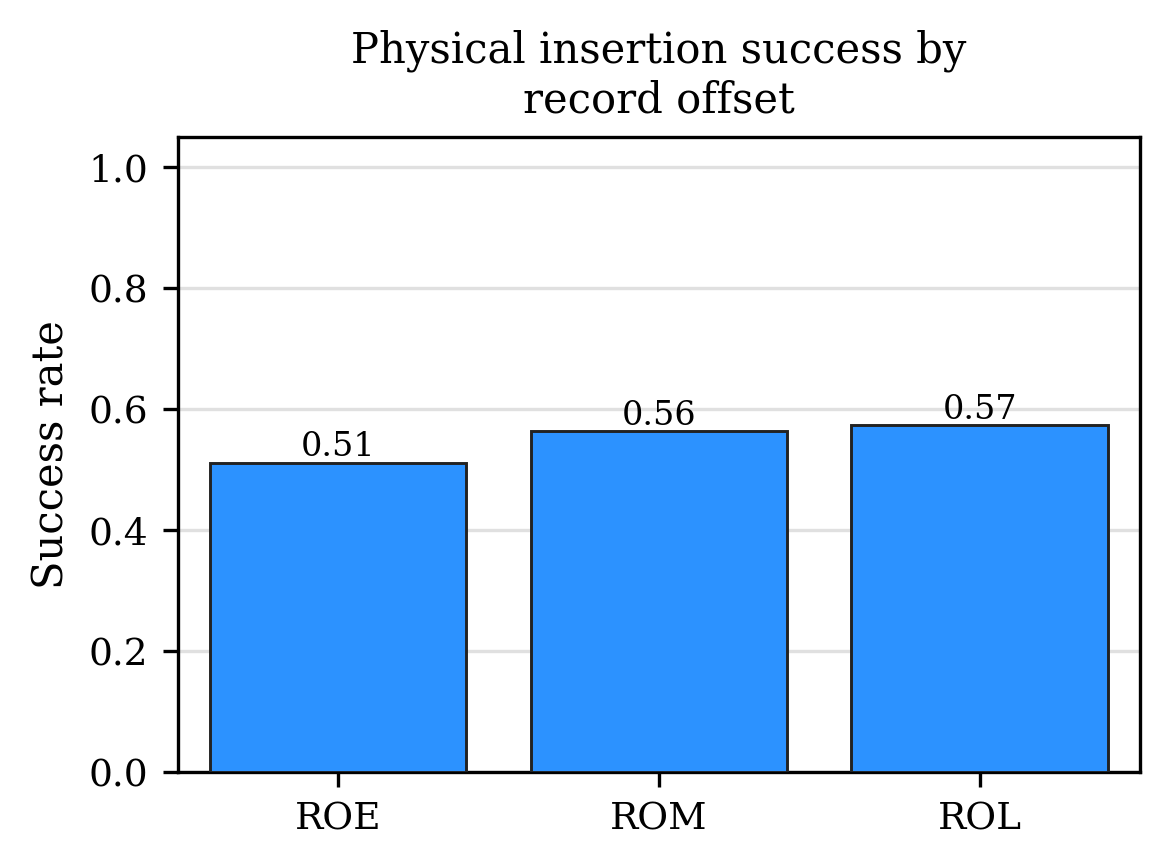
\includegraphics[width=0.9\linewidth]{chapters/7-results/DA1/global/physical_record_offset_global.png}
        \caption{Global physical success rate for record-offset groups.}
        \label{fig:da1_physical_record_offset_global}
    \end{minipage}    
    \hfill
    \begin{minipage}[t]{0.45\textwidth}
        \centering
        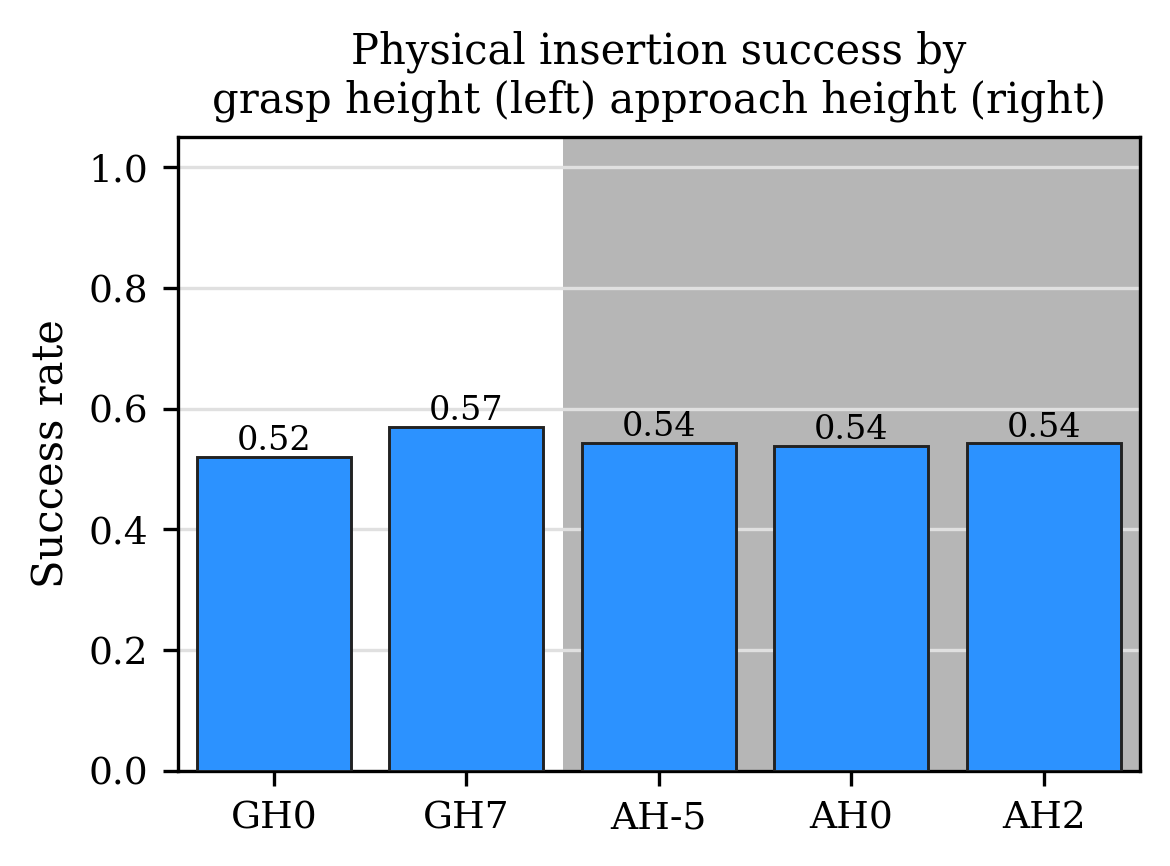
\includegraphics[width=0.9\linewidth]{chapters/7-results/DA1/global/physical_grasp_approach_height_global.png}
        \caption{Global physical success rate for grasp height and approach height.}
        \label{fig:da1_physical_grasp_approach_height_global}
    \end{minipage}    
\end{figure}

\begin{figure}[htbp]
    \centering
    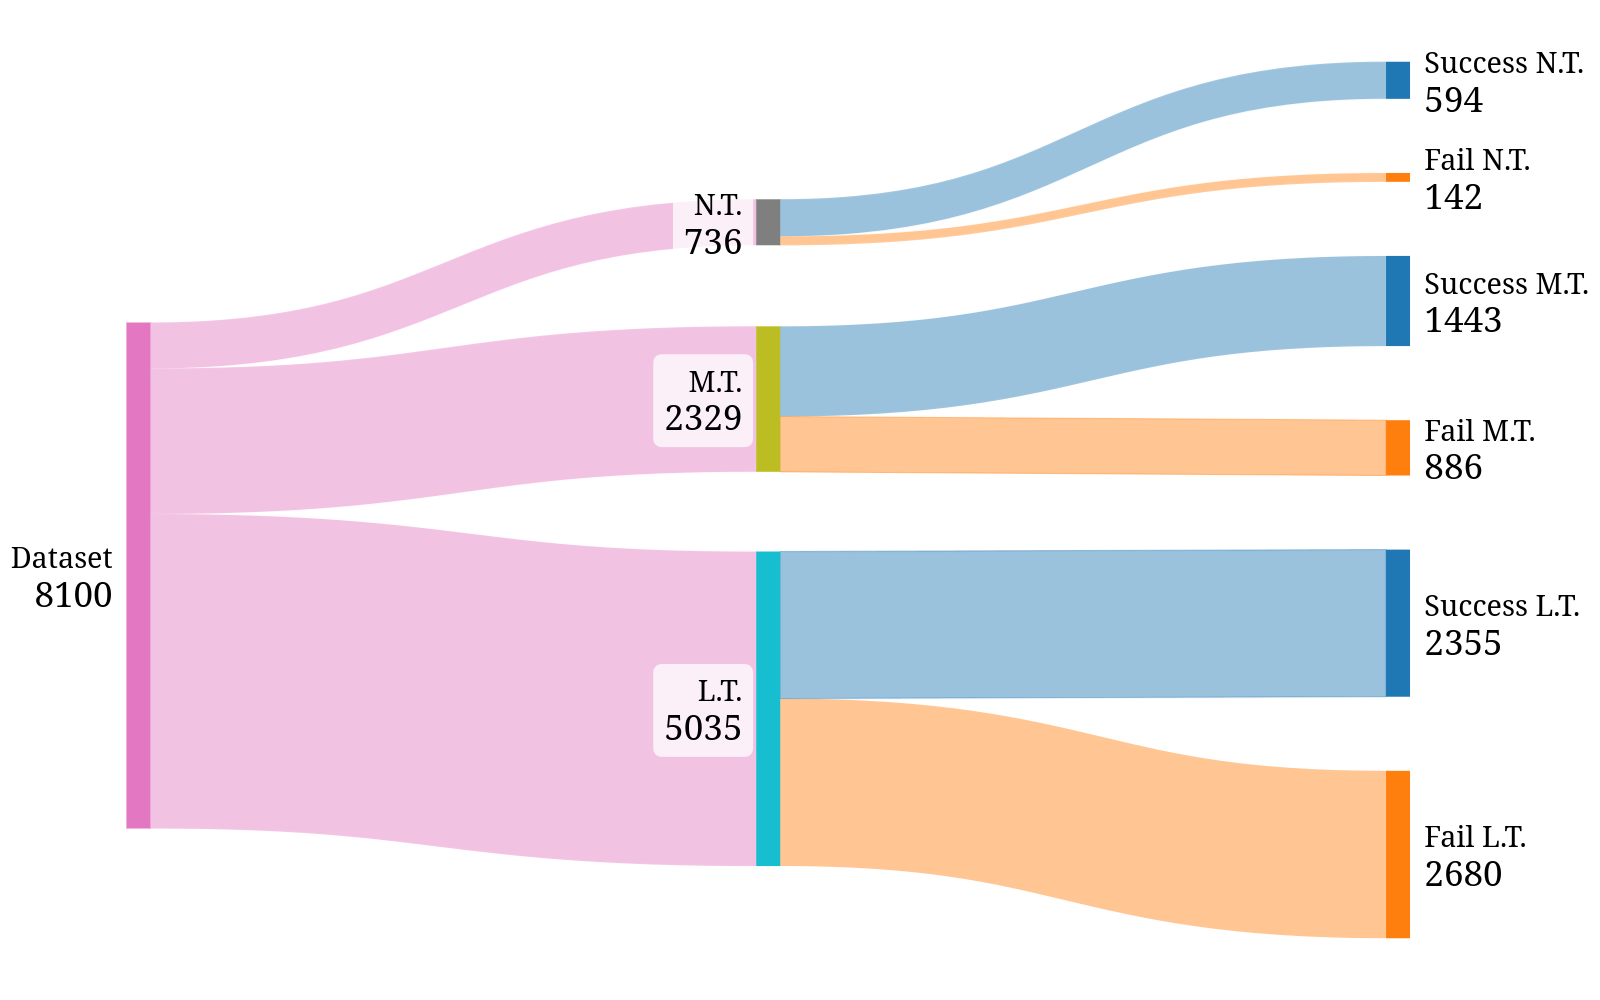
\includegraphics[width=0.8\linewidth]{chapters/7-results/DA1/global/sankey_tilt.png}
    \caption{Example Sankey diagram showing the split of the complete dataset into tilt groups and physical insertion outcomes.}
    \label{fig:da1_sankey_tilt}
\end{figure}

\begin{table}[htbp]
    \centering
    \caption{Sample counts and class balance for the global deviation groups used in Deviation Analysis I.}
    \label{tab:da1_class_split_global}
    \begin{tabular}{l lll lll}
        \toprule
        \textbf{Deviation group} & \textbf{LV} & \textbf{\#} & \textbf{(pos, neg)} & \textbf{LV} & \textbf{\#} & \textbf{(pos, neg)}\\
        \midrule

        \texttt{position} & N.O. & 3150 & (1688, 1462) & M.O. & 2484 & (1429, 1055) \\
        & L.O. & 2466 & (1275, 1191) \\
        \midrule
        \texttt{tilt} & N.T. & 736 & (594, 142) & M.T. & 2329 & (1443, 886) \\
        & L.T. & 5035 & (2355, 2680) \\
        \midrule
        \texttt{offset\_direction} & C & 3150 & (1688, 1462) & pos x & 1328 & (813, 515) \\
        & neg x & 1146 & (545, 601) & pos y & 1319 & (749, 570) \\
        & neg y & 1157 & (597, 560) \\
        \midrule
        \texttt{force\_level} & F15 & 1180 & (682, 498) & F20 & 1220 & (895, 325) \\
        & F25 & 2100 & (1211, 889)  & F30 & 1211& (724, 487) \\
        & F35 & 1200 & (505, 695) & F40 & 1189 & (375, 814) \\
        \midrule
        \texttt{force\_limit} & L30 & 2448 & (1019, 1429) & L40 & 3276 & (2023, 1253) \\
        & L50 & 2376 & (1350, 1026) \\
        \midrule
        \texttt{record\_offset} & ROE & 3780 & (1930, 1850) & ROM & 1440 & (811, 629) \\
        & ROL & 2880 & (1651, 1229) \\
        \midrule
        \texttt{grasp\_height} & 0 mm & 4500 & (2342, 2158) & 7 mm & 3600 & (2050, 1550) \\
        \midrule
        \texttt{approach\_height} & -5 mm & 3649 & (1982, 1667) & 0 mm & 900 & (484, 416) \\
        & 2 mm & 3551 & (1926, 1625) \\
        \midrule
        \texttt{position\_tilt} & N.O. / N.T. & 218 & (193, 25) & N.O. / M.T. & 866 & (523, 343) \\
        & N.O. / L.T. & 2066 & (972, 1094) & M.O. / N.T. & 265 & (230, 35) \\
        & M.O. / M.T. & 1087 & (690, 397) & M.O. / L.T. & 1132 & (509, 623) \\
        & L.O. / N.T. & 253 & (171, 82) & L.O. / M.T. & 376 & (230, 146) \\
        & L.O. / L.T. & 1837 & (874, 963) \\
        \midrule
        \texttt{force\_interaction} & F15 / L30 & 401 & (237, 164) & F15 / L40 & 389 & (271, 118) \\
        & F15 / L50 & 390 & (174, 216) & F20 / L30 & 415 & (340, 75) \\
        & F20 / L40 & 403 & (330, 73) & F20 / L50 & 402 & (225, 177) \\
        & F25 / L30 & 408 & (256, 152) & F25 / L40 & 1296 & (769, 527) \\
        & F25 / L50 & 396 & (186, 210) & F30 / L30 & 411 & (110, 301) \\
        & F30 / L40 & 400 & (346, 54) & F30 / L50 & 400 & (268, 132) \\
        & F35 / L30 & 408 & (64,344) & F35 / L40 & 396 & (230, 166) \\
        & F35 / L50 & 396 & (211, 185) & F40 / L30 & 405 & (12,393) \\
        & F40 / L40 & 392 & (77, 315) & F40 / L50 & 392 & (286, 106) \\
        \midrule
        \figref{fig:da1_physical_force_no_tilt_no_offset} Attributes &
        F15 & 35 & (35, 0) & F20 & 37 & (37, 0) \\
        & F25 & 38 & (38, 0) & F30 & 36 & (36, 0) \\
        & F35 & 36 & (32, 4) & F40 & 36 & (15, 21) \\
        & L30 & 0 & (0, 0) & L40 & 218 & (193, 25) \\
        & L50 & 0 & (0, 0) \\
        \midrule
        \figref{fig:da1_physical_position_tilt_f40_l30} Attributes &
        N.O. / N.T. & 0 & (0, 0) & N.O. / M.T. & 65 & (1, 64) \\
        & N.O. / L.T. & 173 & (5, 168) & M.O. / N.T. & 0 & (0, 0) \\
        & M.O. / M.T. & 25 & (2, 23) & M.O. / L.T. & 56 & (0, 56) \\
        & L.O. / N.T. & 0 & (0, 0) & L.O. / M.T. & 19 & (1, 18) \\
        & L.O. / L.T. & 67 & (3, 64) \\
        \bottomrule
    \end{tabular}
\end{table}

\subsection{Domain specific Investigation of Deviation Groups}
\label{subsec:da1_domain_investigation}

The global investigation identified tilt magnitude, offset direction, and force interaction as the most informative deviation groups for the physical success-rate analysis. These groups are therefore investigated further on selected dataset domains. The purpose of this second part is to determine whether the global effects are consistent across hole configurations, or whether they are caused by specific rod--tolerance combinations, gripper configurations, or batch-dependent recording conditions.

The analysis is focused on the hole domains, defined by the combination of \texttt{rod\_type} and \texttt{tolerance}. Additional focused investigations are then performed for domains that show particularly strong or unexpected behavior.

\subsubsection{Hole-Domain Screening}
\label{subsubsec:da1_hole_domain_screening}

\figref{fig:da1_domain_position_tilt_holes} shows the physical success rate of the individual position-offset and tilt groups across the nine hole domains. The domain-specific view confirms the global observation that tilt is more impactful than position offset alone. Across most hole domains, the no-tilt group has the highest success rate, while large tilt causes the success rate to drop. 8 out of 9 hole domains follow the consisten trend:

\begin{equation}
    \text{SR}(\texttt{N.T.}) > \text{SR}(\texttt{M.T.}) > \text{SR}(\texttt{L.T.})
    \qquad
    \text{SR}() := \texttt{Success Rate()}.
    \label{eq:tilt_trend}
\end{equation}
\texttt{small\_rod\_t0.2} is the only case where $\text{SR}(\texttt{M.T.}) < \text{SR}(\texttt{L.T.})$.

In contrast, the position-offset groups do not show the same consistent decline of success rate. No offset is not always clearly superior to moderate or large offset, which indicates that positional offset magnitude alone is not sufficient to explain the physical outcome.

The combined position--tilt groups in \figref{fig:da1_domain_position_over_tilt_holes} provide a more detailed view of this effect. The highest success rates occur mostly in groups where no-tilt is involved, especially for the no-offset with no-tilt case. However, the effect is not identical in all hole domains. Some combinations are missing due to the deterministic structure of the deviation planner, and some domains show local patterns that differ from the global trend. In particular, \texttt{small\_rod\_t0.3} shows no samples for \texttt{M.O. / N.T.} and a very low success rate for \texttt{M.O. / L.T.}. 

\figref{fig:da1_domain_offset_direction_holes} shows the hole domain specific view on the success rate of the five offset-directions. The domain \texttt{small\_rod\_t0.3} shows unexpected behavior, where offsets in the negative $x$ and negative $y$ directions are associated with much lower success rates than offsets in the positive directions. This could reveal a directional bias or asymmetry in the robotic setup. If the targeted insertion pose without deviations applied, is slightly shifted relative to the ground truth hole center, repeated deviations in one direction can show different behavior than deviations in the opposite direction.

Because of these two anomalies regarding \texttt{small\_rod\_t0.3}, this domain is further investigated in Section \ref{subsubsec:da1_small_rod_t03_directional_bias}.

The force-interaction heatmap in \figref{fig:da1_domain_force_interaction_holes} shows particularly stronger variation across hole domains. The combination \texttt{F40 / L30} remains one of the least successful settings across several hole domains, which is consistent with the global result in \figref{fig:da1_physical_force_interaction_global}. This setting combines the highest commanded force level with the lowest force limit, so the force limit is likely to be reached before the insertion can be completed. At the same time, the heatmap shows that the force interaction global pattern does not apply to all hole domains. The \texttt{rect\_rod\_t0.1} domain in particular shows extreme differences, with some force interactions leading to almost complete success (\texttt{F20 / L40}) with direclty adjacent force interactions leading to almost complete failure (\texttt{F20 / L50}). This motivated the second focused investigation of \texttt{rect\_rod\_t0.1} in Subsection \ref{subsubsec:da1_rect_rod_t01_force_modes}.

\begin{figure}[htbp]
    \centering
    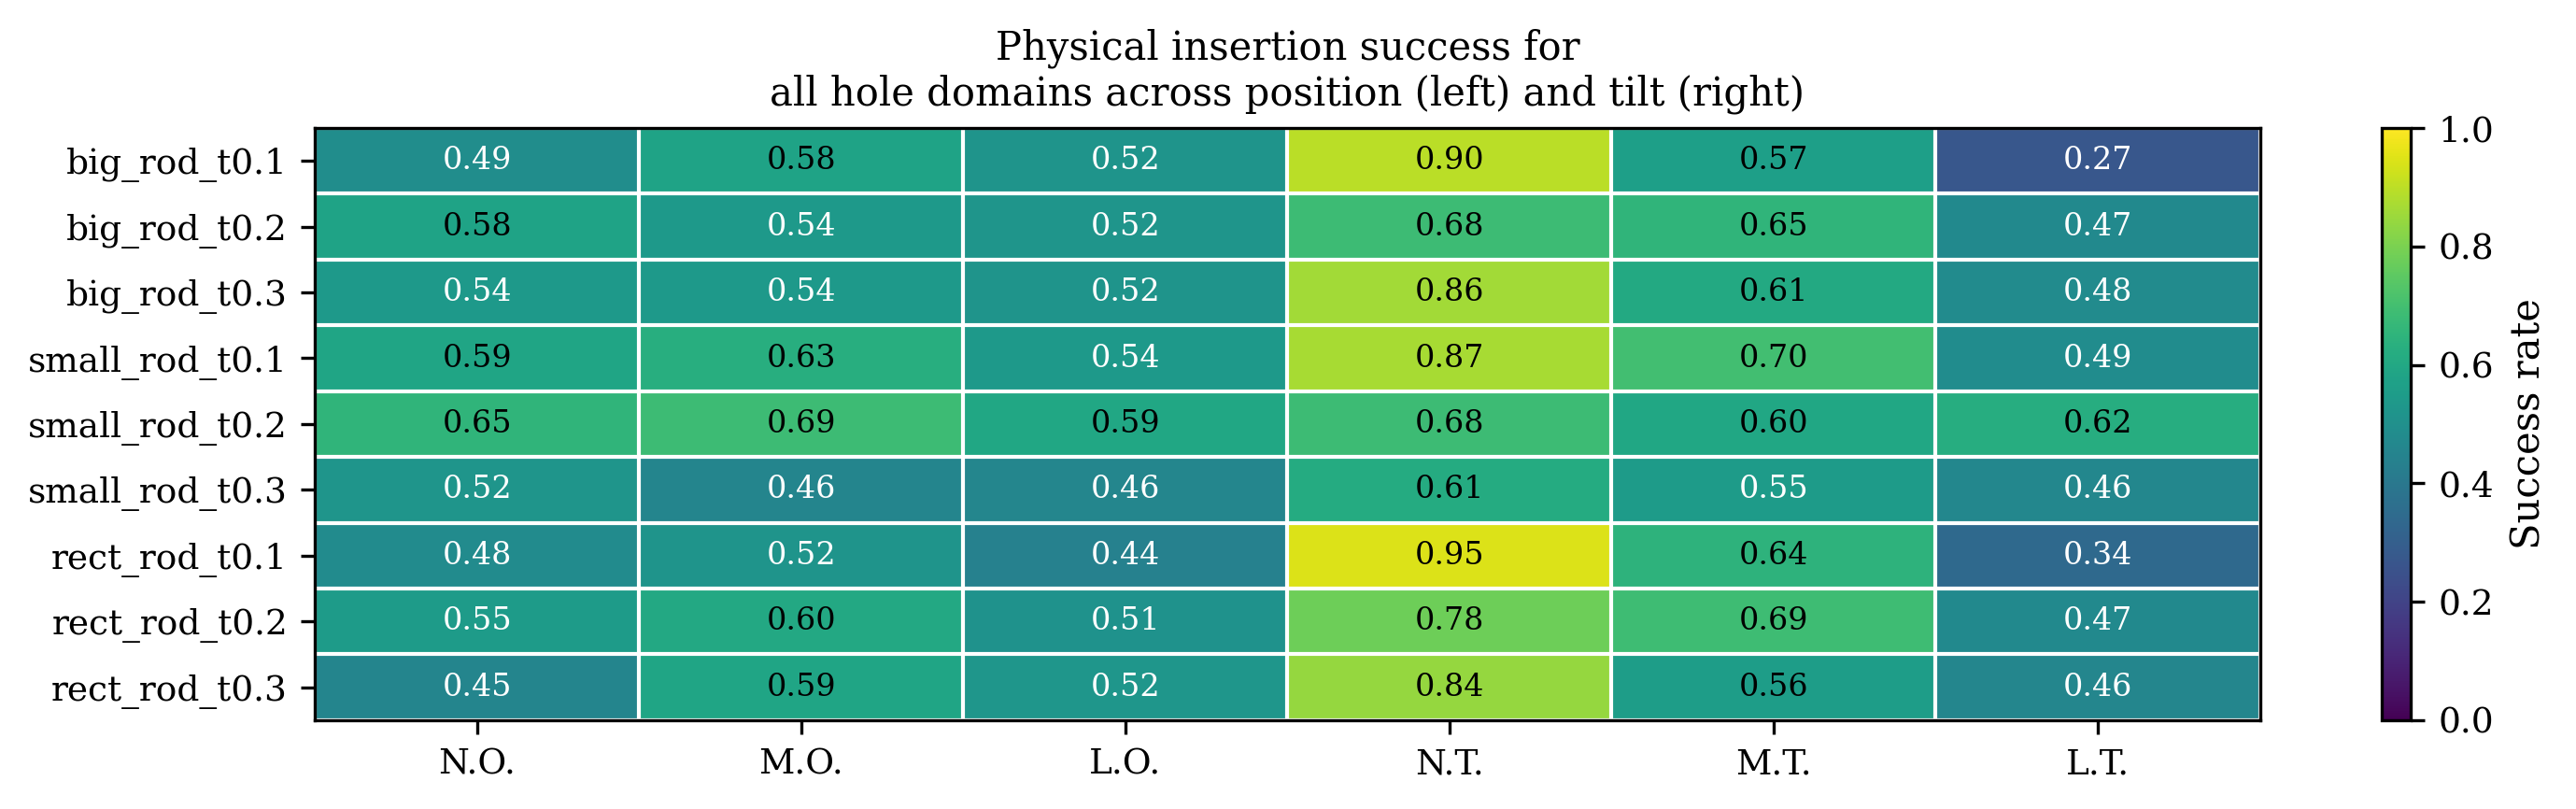
\includegraphics[width=0.95\linewidth]{chapters/7-results/DA1/domain/physical_hole_domains_position_and_tilt.png}
    \caption{Physical success rate of position-offset and tilt groups across all hole domains.}
    \label{fig:da1_domain_position_tilt_holes}
\end{figure}

\begin{figure}[htbp]
    \centering
    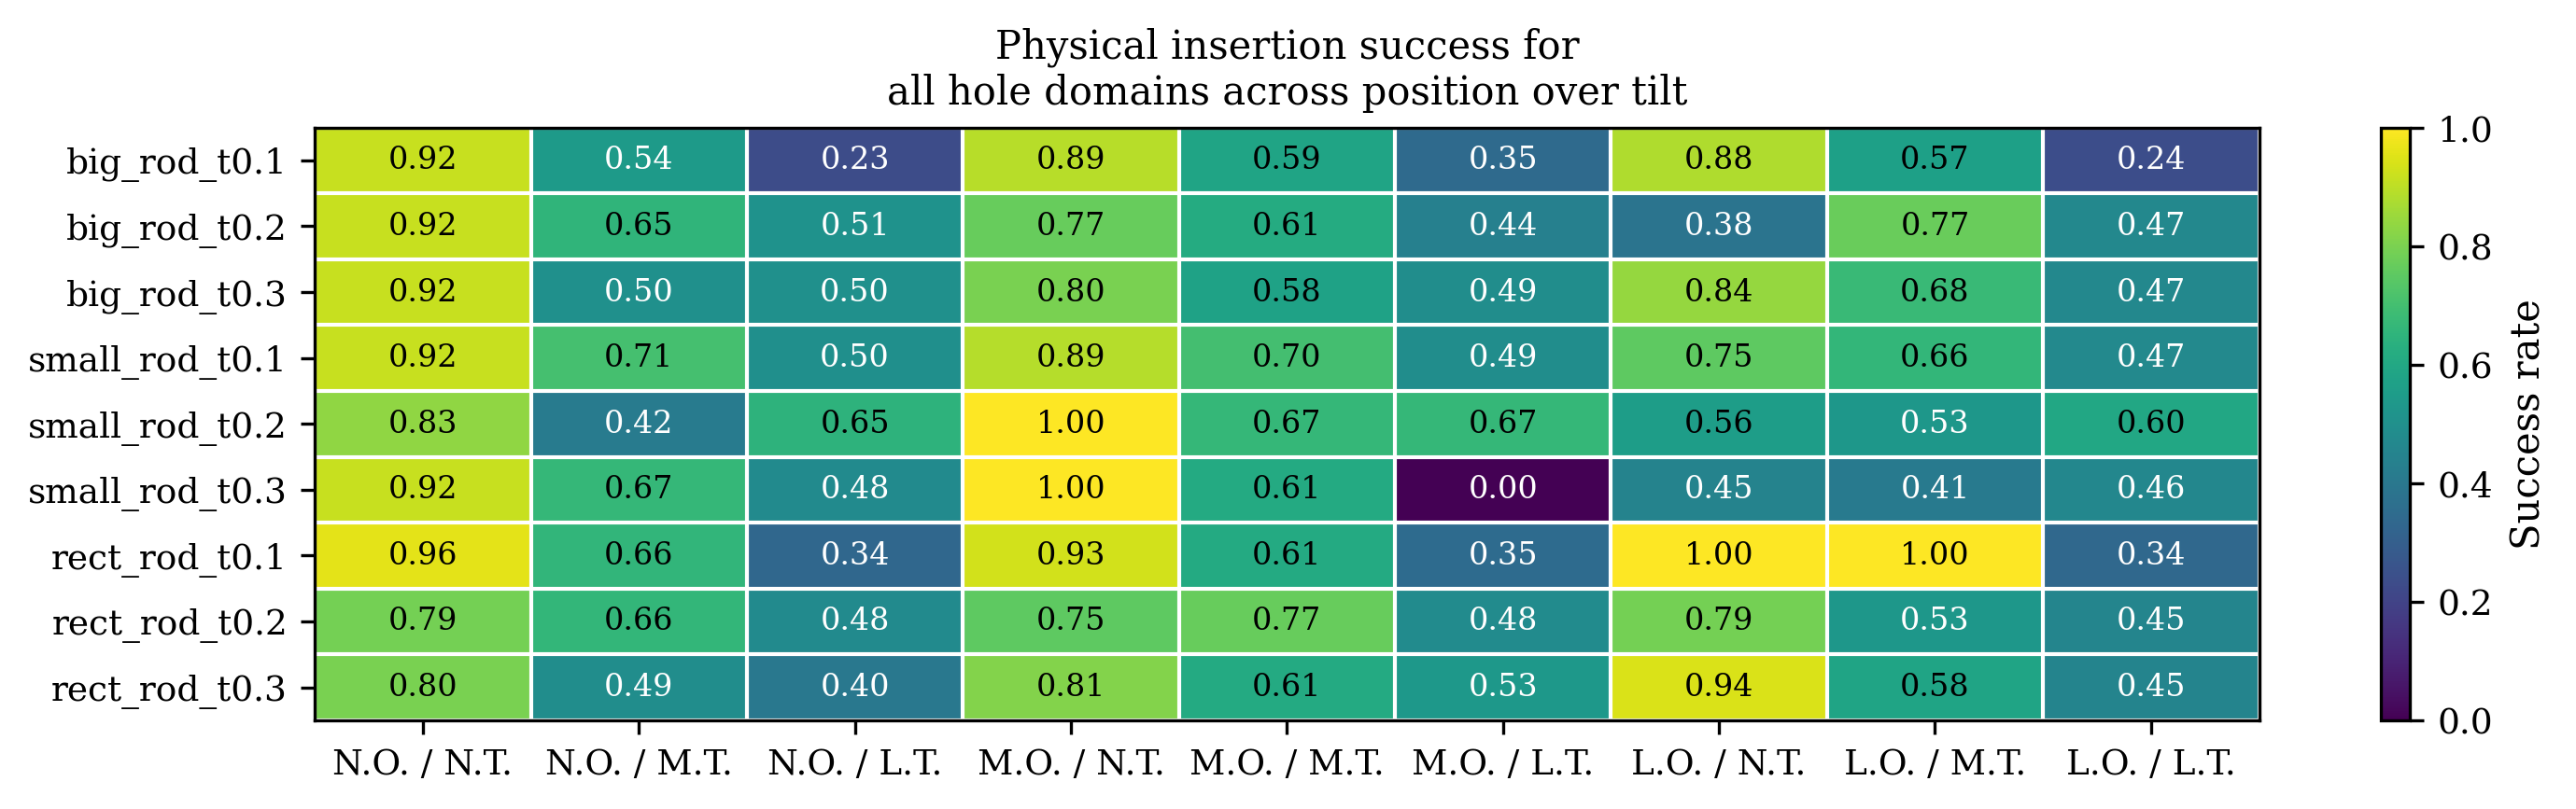
\includegraphics[width=0.95\linewidth]{chapters/7-results/DA1/domain/physical_hole_domains_position_over_tilt.png}
    \caption{Physical success rate of combined position--tilt groups across all hole domains.}
    \label{fig:da1_domain_position_over_tilt_holes}
\end{figure}

\begin{figure}[htbp]
    \centering
    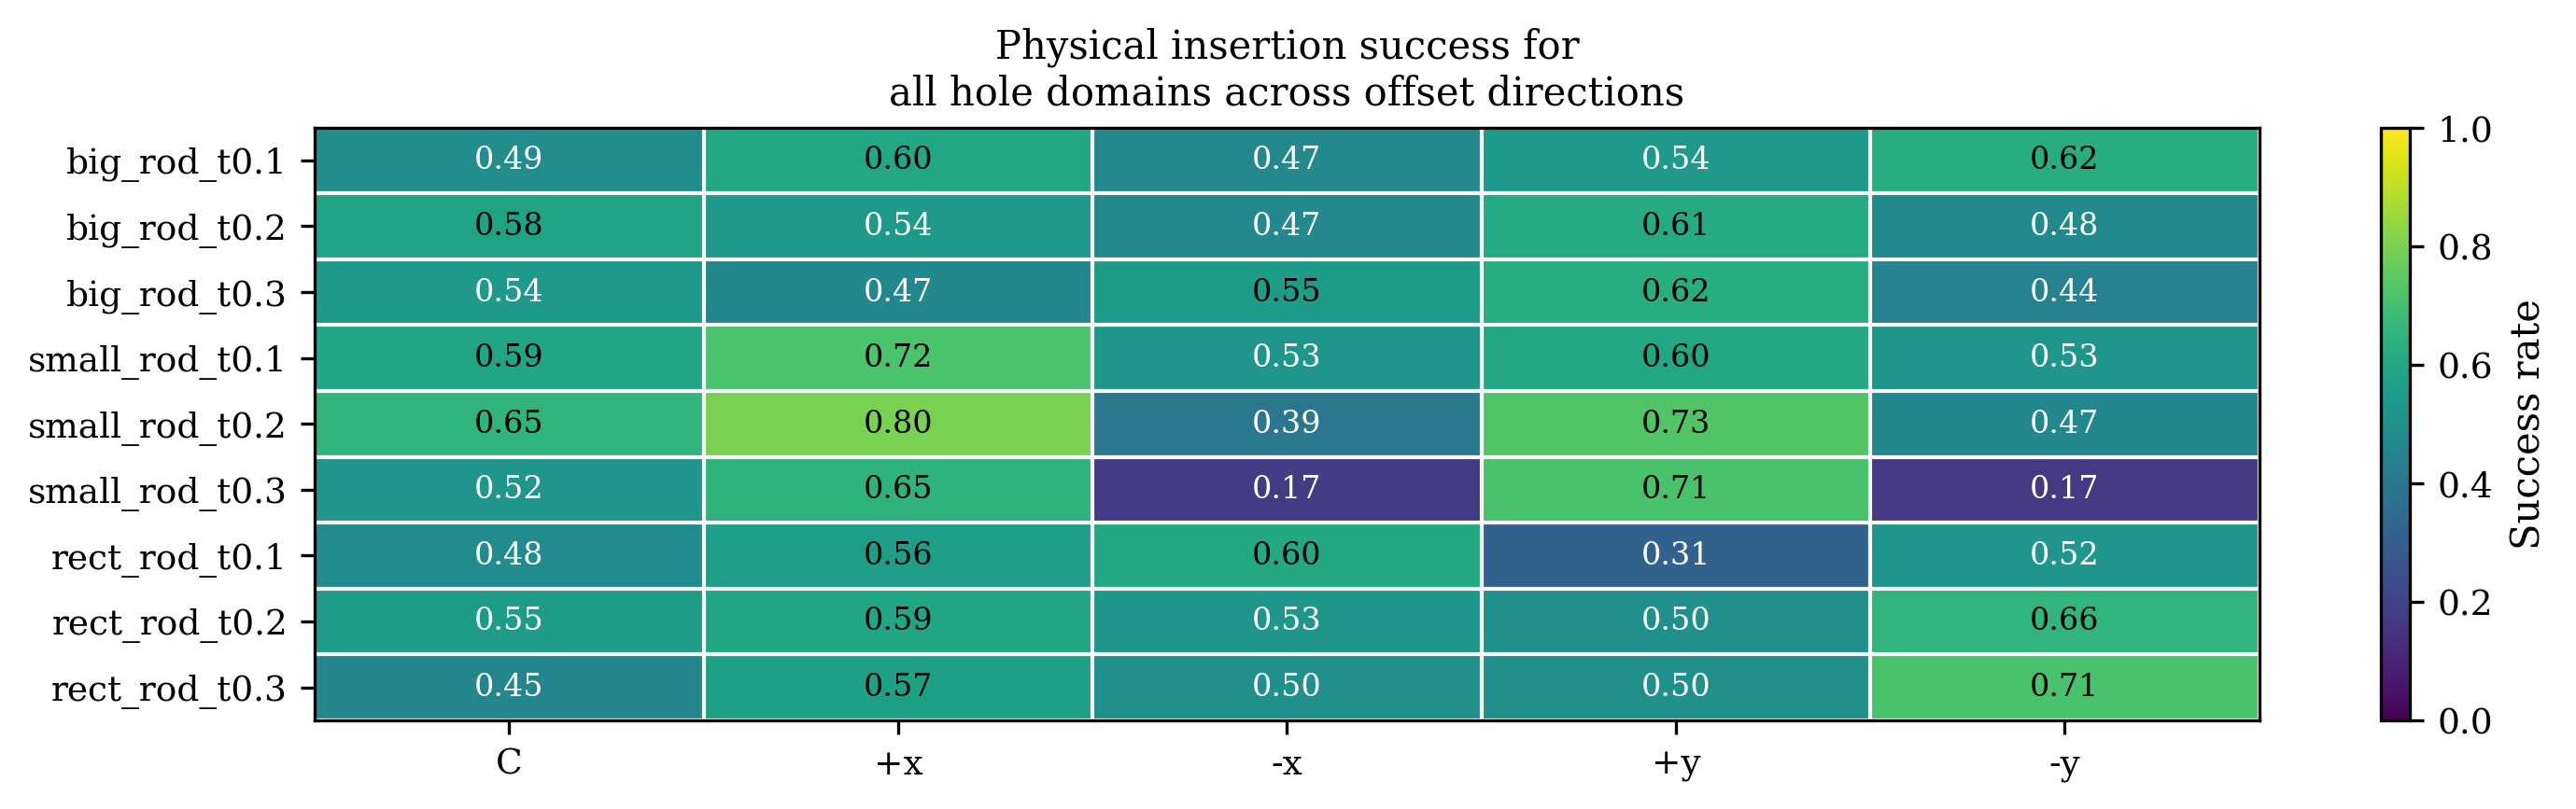
\includegraphics[width=0.95\linewidth]{chapters/7-results/DA1/domain/physical_hole_domains_offset_direction.png}
    \caption{Physical success rate of offset-direction groups across all hole domains.}
    \label{fig:da1_domain_offset_direction_holes}
\end{figure}

\begin{figure}[htbp]
    \centering
    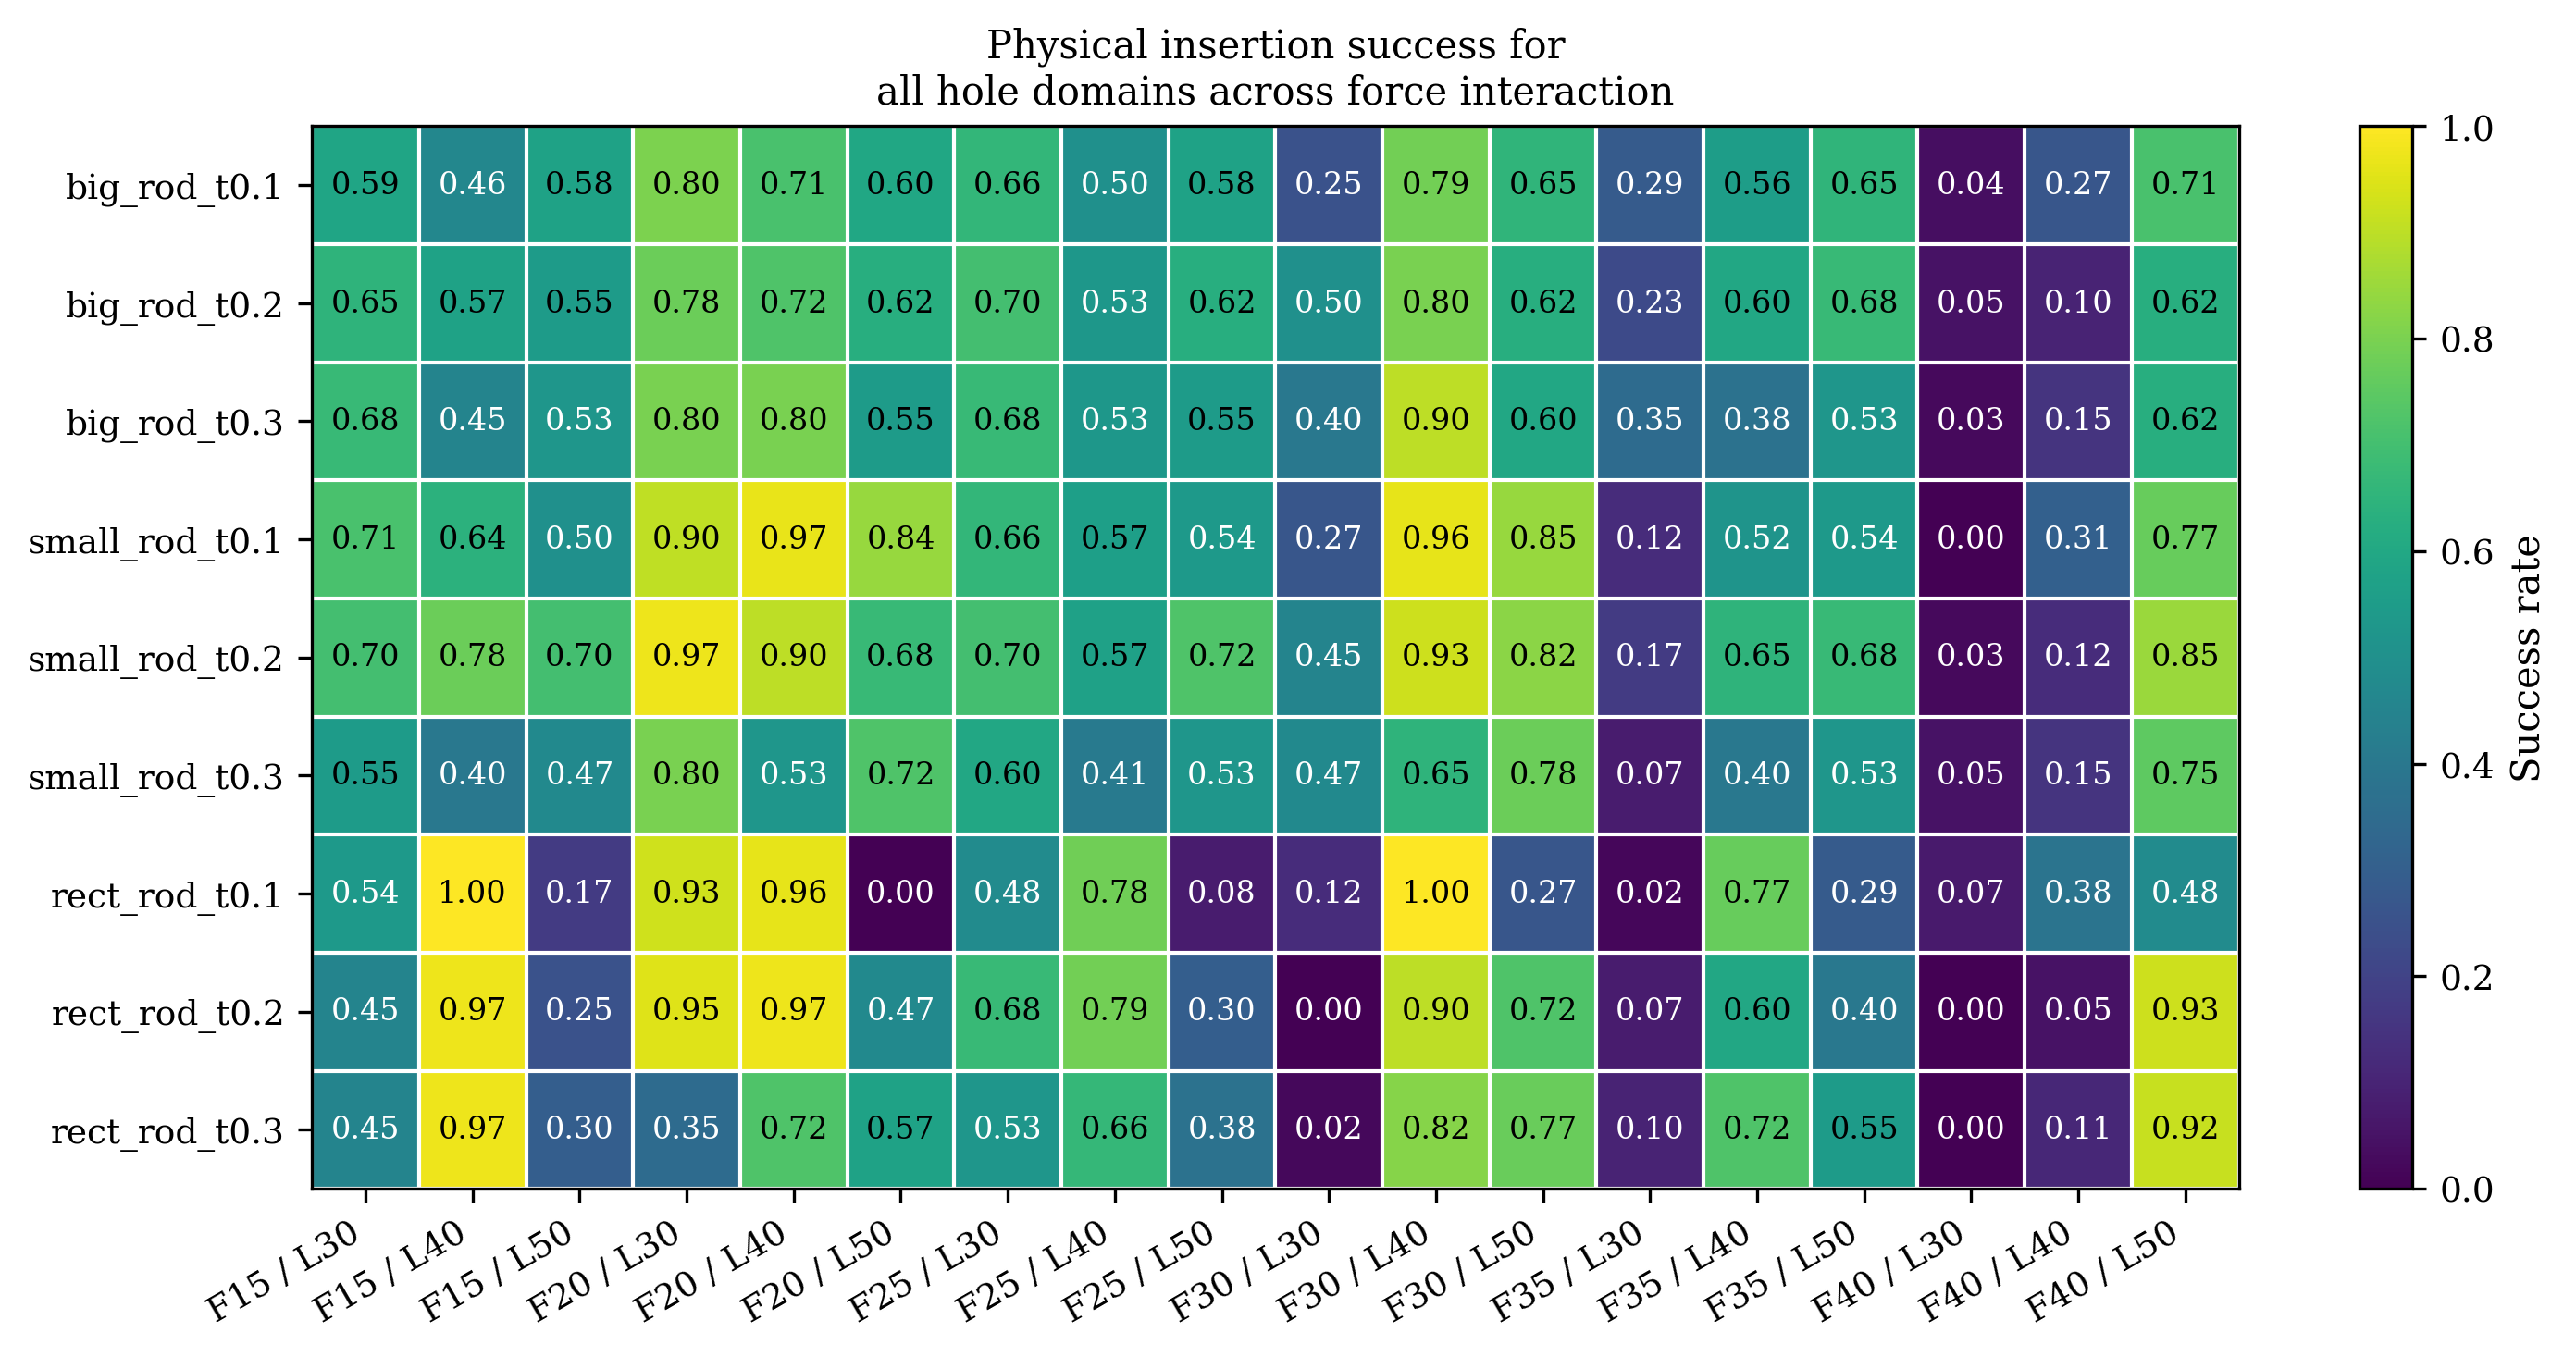
\includegraphics[width=0.95\linewidth]{chapters/7-results/DA1/domain/physical_hole_domains_force_interaction.png}
    \caption{Physical success rate of force-interaction groups across hole domains.}
    \label{fig:da1_domain_force_interaction_holes}
\end{figure}

For the focused investigations, the heatmap tiles are extended with additional failure-mode information. This comes from the metadata entry \texttt{failure\_reason} in \tabref{tab:recorded_metadata} and its description in Section \ref{sec:dataset_labeling}. Besides the success rate, each tile reports the number of samples $n$ and the distribution of failure reasons. The abbreviation \texttt{T} denotes the count of timeouts, \texttt{F} denotes the count of force-limit reached failures, and \texttt{S} counts the amounf of stall/jam failures. These failure modes allow the success rate to be interpreted more precisely, because a failed insertion can result from different physical mechanisms.

\subsubsection{Directional Bias in \texttt{small\_rod\_t0.3}}
\label{subsubsec:da1_small_rod_t03_directional_bias}

The offset-direction result for \texttt{small\_rod\_t0.3} is investigated in more detail in \figref{fig:da1_small_rod_t03_offset_direction_batch}. The first recorded \texttt{batch\_1} shows a more uniform distribution of offset directions. This is not the case for the later batches, where the asymmetry becomes apparent. This is consistent with the data collection procedure, where in \texttt{batch\_1}, position and orientation deviations were applied more randomly, which can produce individual outliers but does not repeatedly test the same deviation direction with the same offset magnitude. In \texttt{batch\_2} and \texttt{batch\_3}, the deviation planner generated more structured and repeated deviations, so a systematic positional bias becomes more visible.

The distinction between gripper types must be interpreted carefully here. The \texttt{flat} gripper only occurs in \texttt{batch\_3}, while the \texttt{round} gripper is essentially a weighted average of \texttt{batch\_2} and \texttt{batch\_3}. Therefore, the apparent gripper effect is partly coupled with the batch structure and should not be interpreted independently.

\figref{fig:da1_small_rod_t03_offset_direction_detailed} focuses on the negative $x$ and negative $y$ directions and separates them by offset and tilt magnitude, not combined. Since centered samples are assigned to the centered group \texttt{C}, no-offset cases are not shown for the directional groups. For the negative $x$ direction, the success rate decreases with increasing offset magnitude, which is consistent with the fact that large positional deviations cause make failures more likely. Counterintuitively however, does the no-tilt group in the negative $x$ direction show 0\% success rate. One possible explanation is that, for this specific hole domain and direction, if a tilted rod hits the edge of the hole it can guide itself into the opening, while an untilted rod may hit the top surface of the taskboard more directly and stalls completely. Since for this domain the tolerance is the largest level (\texttt{t0.3}), after a possible self-alignment, the robot can successfully continue the insertion under moderate or large tilt.

The failure-cause annotations support the interpretation that the negative-direction failures are not caused by a single mechanism alone. The failures include force-limit terminations, timeouts, and stall/jam detections. This suggests that the directional bias changes the contact situation in several ways. From a practical perspective, this result is useful, because it suggests a possible correction of the physical insertion setup. Because repeated failures occur mainly for negative $x$ and negative $y$ offsets, the starting pose of an insertion without deviations applied could be shifted slightly in the opposite direction, towards the true hole center, to improve insertion reliability.

\begin{figure}[htbp]
    \centering
    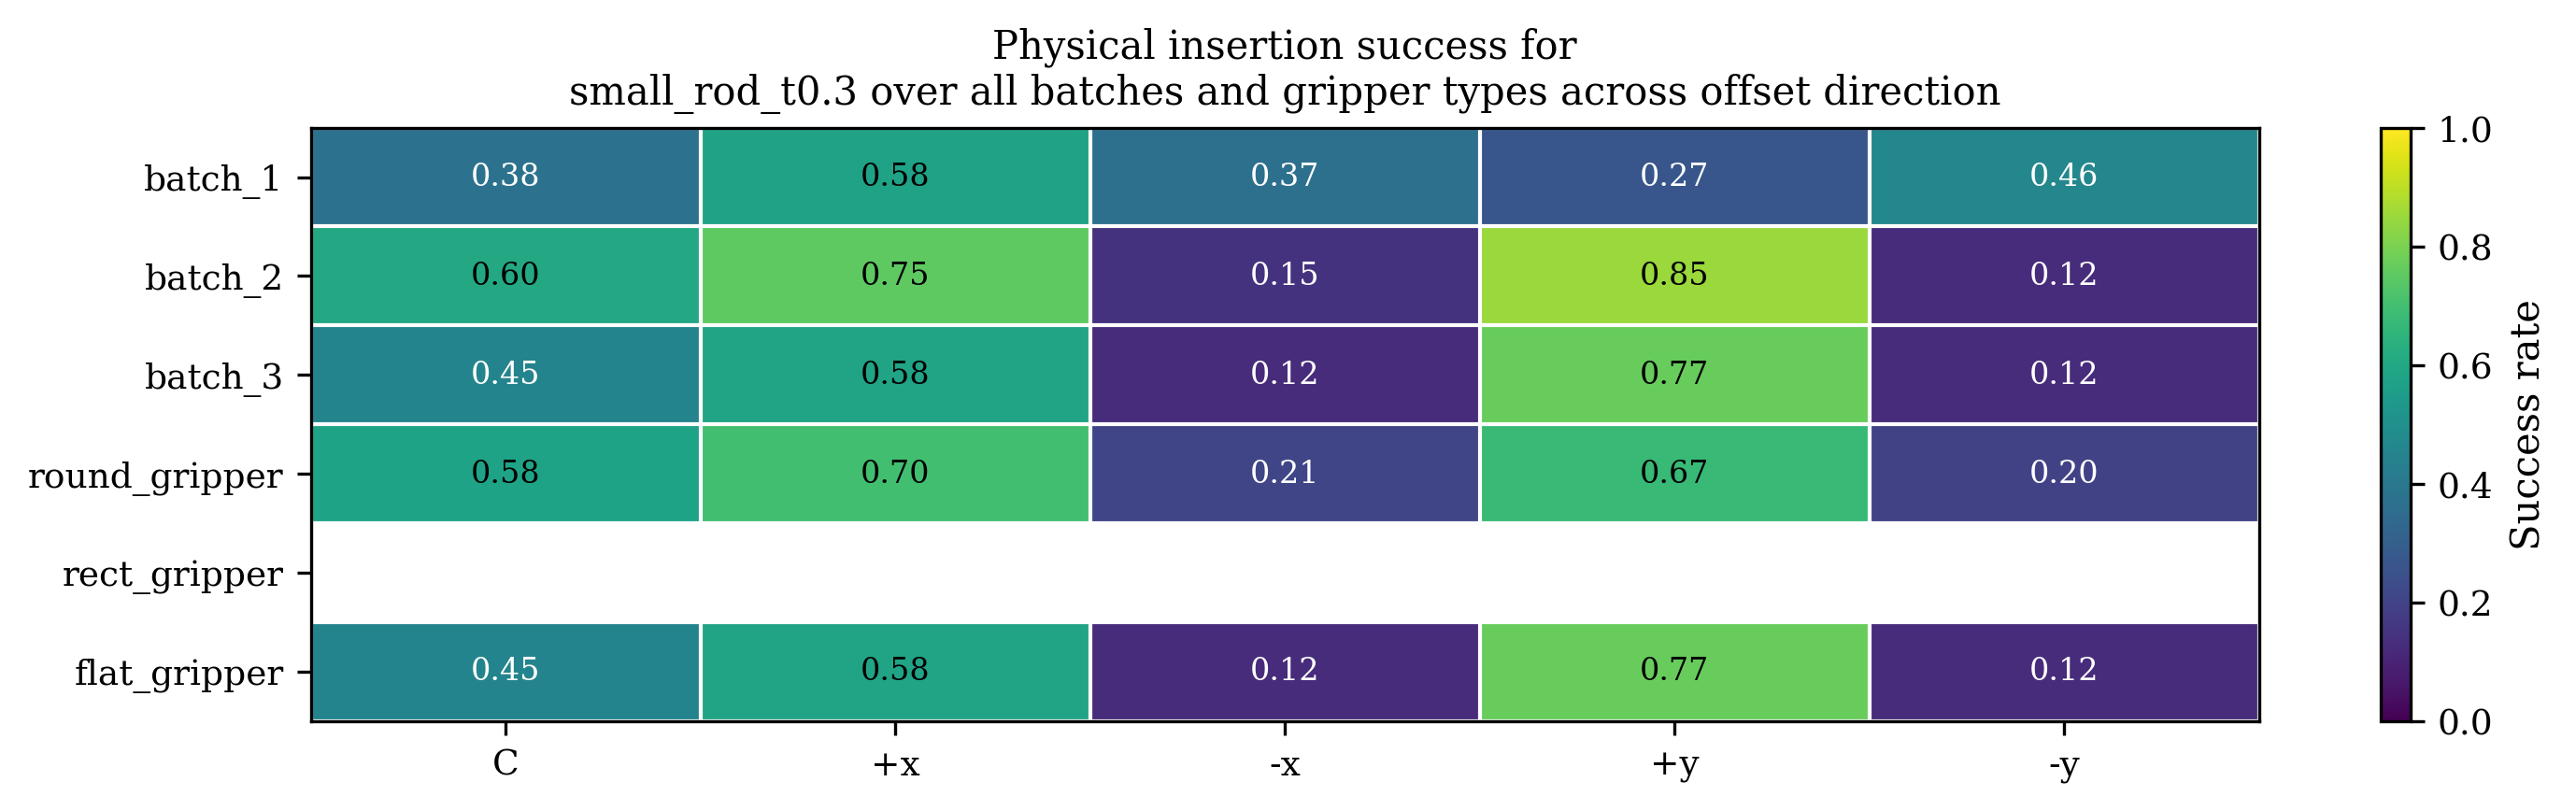
\includegraphics[width=0.95\linewidth]{chapters/7-results/DA1/domain/physical_small_rod_t0.3_batch_gripper_domains_offset_direction.png}
    \caption{Physical success rate of offset-direction groups for \texttt{small\_rod\_t0.3}, separated by batch and gripper domains.}
    \label{fig:da1_small_rod_t03_offset_direction_batch}
\end{figure}

\begin{figure}[htbp]
    \centering
    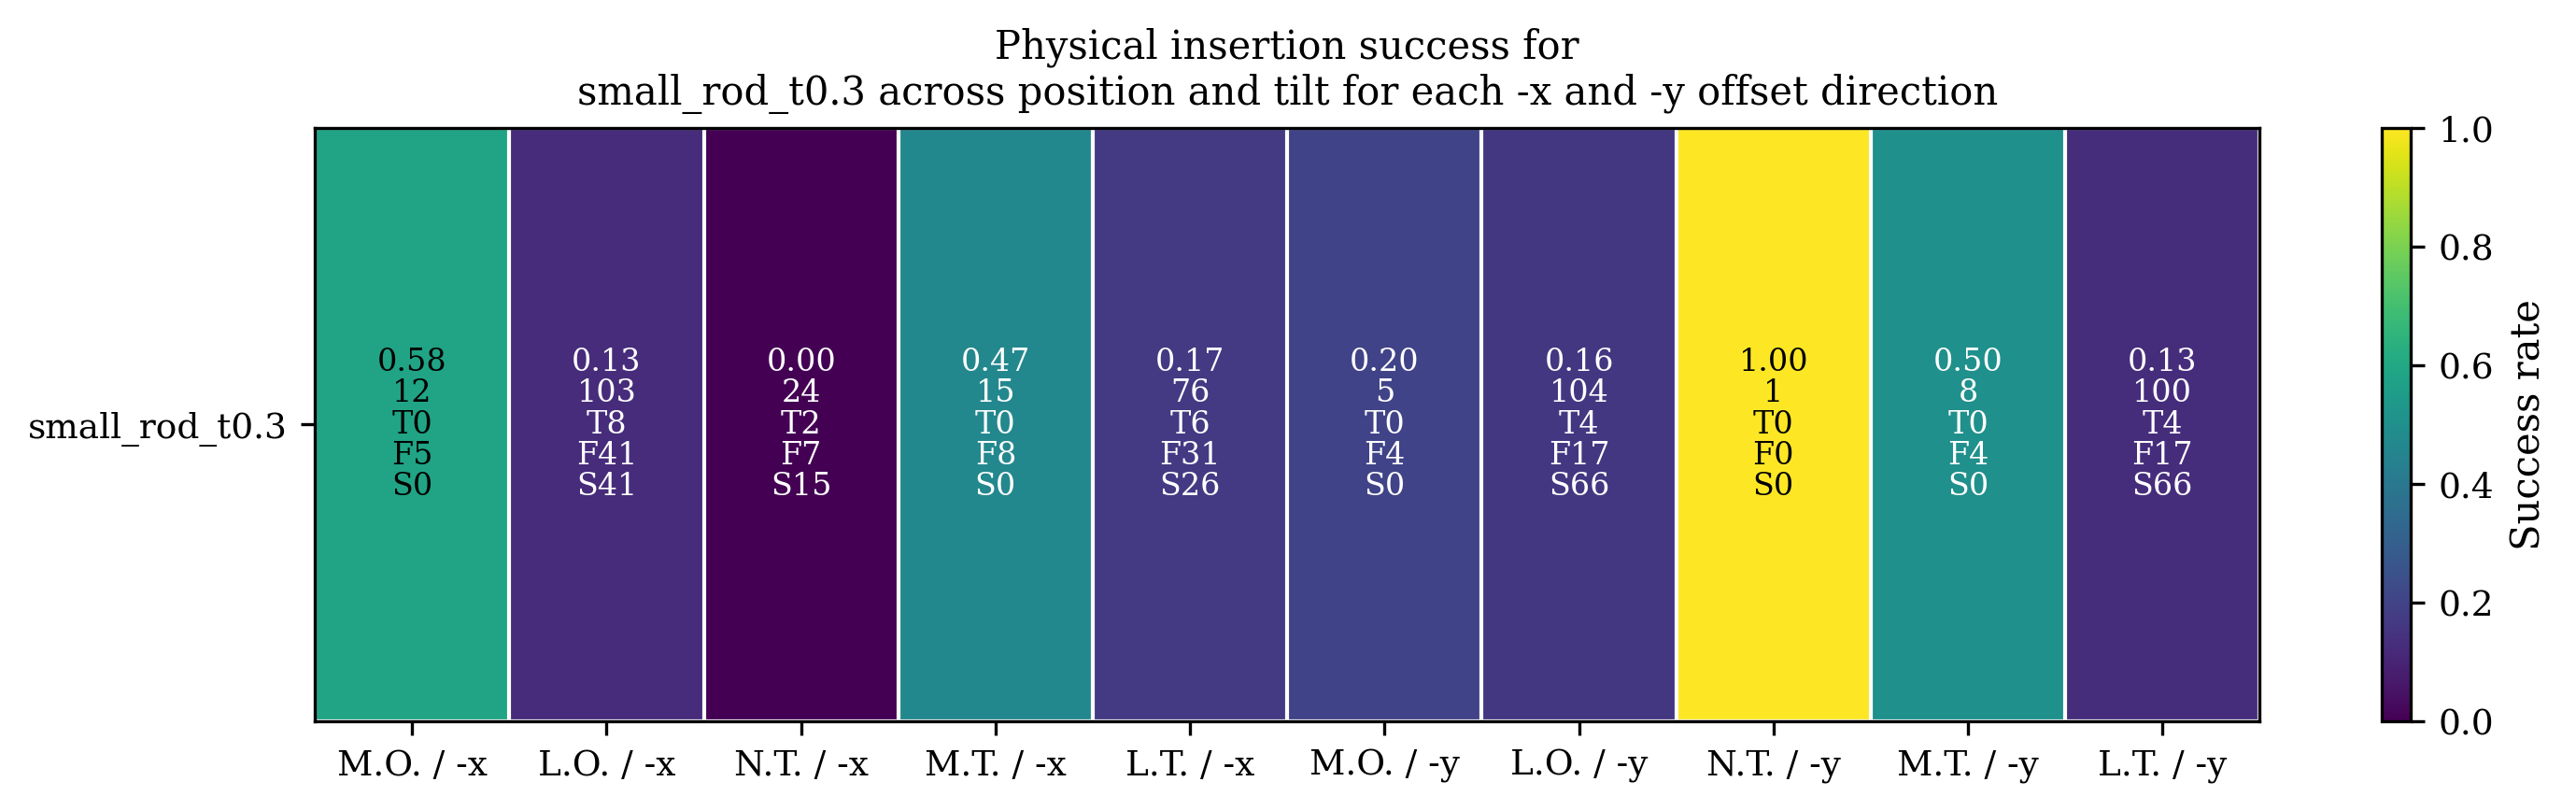
\includegraphics[width=0.95\linewidth]{chapters/7-results/DA1/domain/physical_small_rod_t0.3_domains_offset_direction_3.png}
    \caption{Detailed physical success rate of negative offset directions for \texttt{small\_rod\_t0.3}, separated by offset magnitude and tilt magnitude. Tile annotations include sample counts and failure reasons. N.O. not inlcluded, because the are not associated with a direction, they lie in group \texttt{C}.}
    \label{fig:da1_small_rod_t03_offset_direction_detailed}
\end{figure}



\subsubsection{Failure-Mode Analysis for \texttt{rect\_rod\_t0.1}}
\label{subsubsec:da1_rect_rod_t01_force_modes}

The hole-domain investigation also identified \texttt{rect\_rod\_t0.1} as an unusual case for the force-interaction groups. This domain is analyzed in more detail in \figref{fig:da1_rect_rod_t01_force_interaction_failure_modes}. The plot separates all insertions from the \texttt{rect\_rod\_t0.1} domain in the \texttt{rect\_gripper} and \texttt{flat\_gripper} domains. This separation also reflects the batch structure, where the rectangular gripper was used in \texttt{batch\_1} and \texttt{batch\_2}, while the flat gripper was exclusively used in \texttt{batch\_3}. Therefore, the observations made, are also gripper- and batch-dependent.

The failure-cause annotations explain the extreme variation seen in the global force-interaction heatmap. Force interactions with a small or negative force difference, such as \texttt{F30/L30}, \texttt{F35/L30}, \texttt{F40/L30}, and \texttt{F40/L40}, fail mainly due to the force limit exceeded. This is expected, because if the insertion force is close to or above the allowed force limit, the insertion is terminate before it can be completed. These cases support the interpretation that the difference between force limit and force level is a deciding factor of whether or not the insertion succeeds.

However, increasing the force limit does not automatically make the insertion successful. Several force interactions with a positive (positive and far from zero) force difference still show low success rates, but their dominant failure cause changes. Instead of force-limit termination, the failures are mainly caused by stall/jam, visible for \texttt{F20 / L50}, \texttt{F25 / L50}, \texttt{F30 / L50} and \texttt{F35 / L50}. This indicates that a higher force limit can prevent early timeout termination, but can also allow the system to continue pushing further into a stall or jam. In particular, force limit and stall/jam failure occur in opposite ways, when there are a lot of force limit caused failures, the stall/jam caused failure rate is very low, effectively zero, and vise-versa. The only exception is for \texttt{F25 / L30}. Therefore, force-limit failures and stall/jam failures must be interpreted as different physical mechanisms.

Low commanded force levels show another failure mechanism. In some \texttt{F15} cases, a notable number of failures are timeouts. This is consistent with the interpretation that the insertion velocity slows down with lower force levels and the insertion may not finish within the 3s sequence window.

Therefore the force difference is a crucial metric to explain failures caused by force limit versus failures caused by Stall/jam. Especially low forces however can fail because the insertion velocity is too slow, reaching a timeout.

% One initially surprising observation is the strong difference between \texttt{F20/L40} and \texttt{F20/L50}. This should not be interpreted as an isolated negative effect caused only by the 50 N force limit. The additional position--tilt split in \figref{fig:da1_rect_rod_t01_position_tilt_force_check} is restricted to \texttt{F20} over all force limits. It shows that the force-interaction groups are not paired with identical geometric deviation conditions. Instead, the deterministic deviation planner couples force settings with position and tilt deviations. In this case, the low success rate of \texttt{F20/L50} is better explained by its association with unfavorable tilt and offset conditions than by the force limit alone.

This focused investigation shows why the force-interaction results must be interpreted carefully. The global heatmap correctly identifies force interaction as an important deviation group, but the underlying failure modes and coupled deviations determine whether a low success rate is caused by force-limit termination, timeout, or stall/jam.

\begin{figure}[htbp]
    \centering
    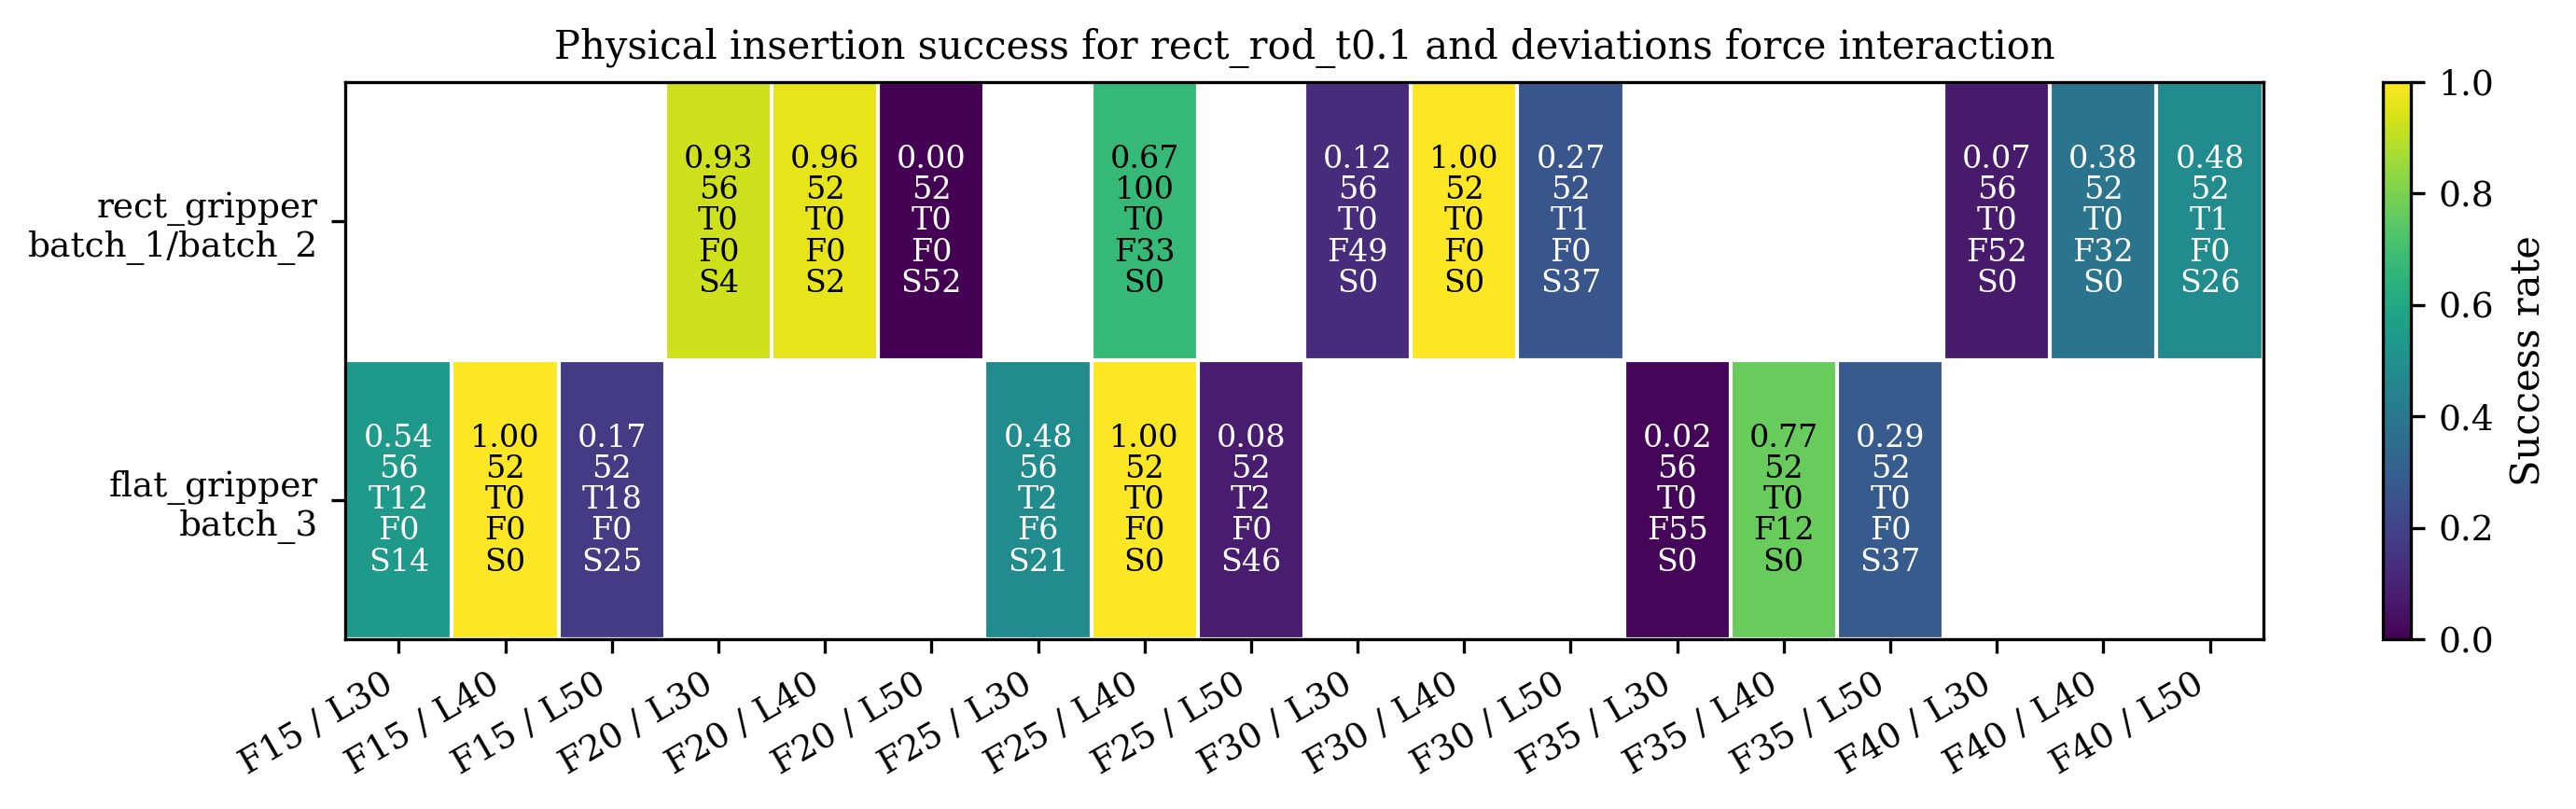
\includegraphics[width=0.95\linewidth]{chapters/7-results/DA1/domain/physical_rect_rod_t0.1_domains_force_interaction_4.png}
    \caption{Detailed physical success rate of force-interaction groups for \texttt{rect\_rod\_t0.1}. Tile annotations include sample counts and failure reasons.}
    \label{fig:da1_rect_rod_t01_force_interaction_failure_modes}
\end{figure}

% \begin{figure}[htbp]
%     \centering
%     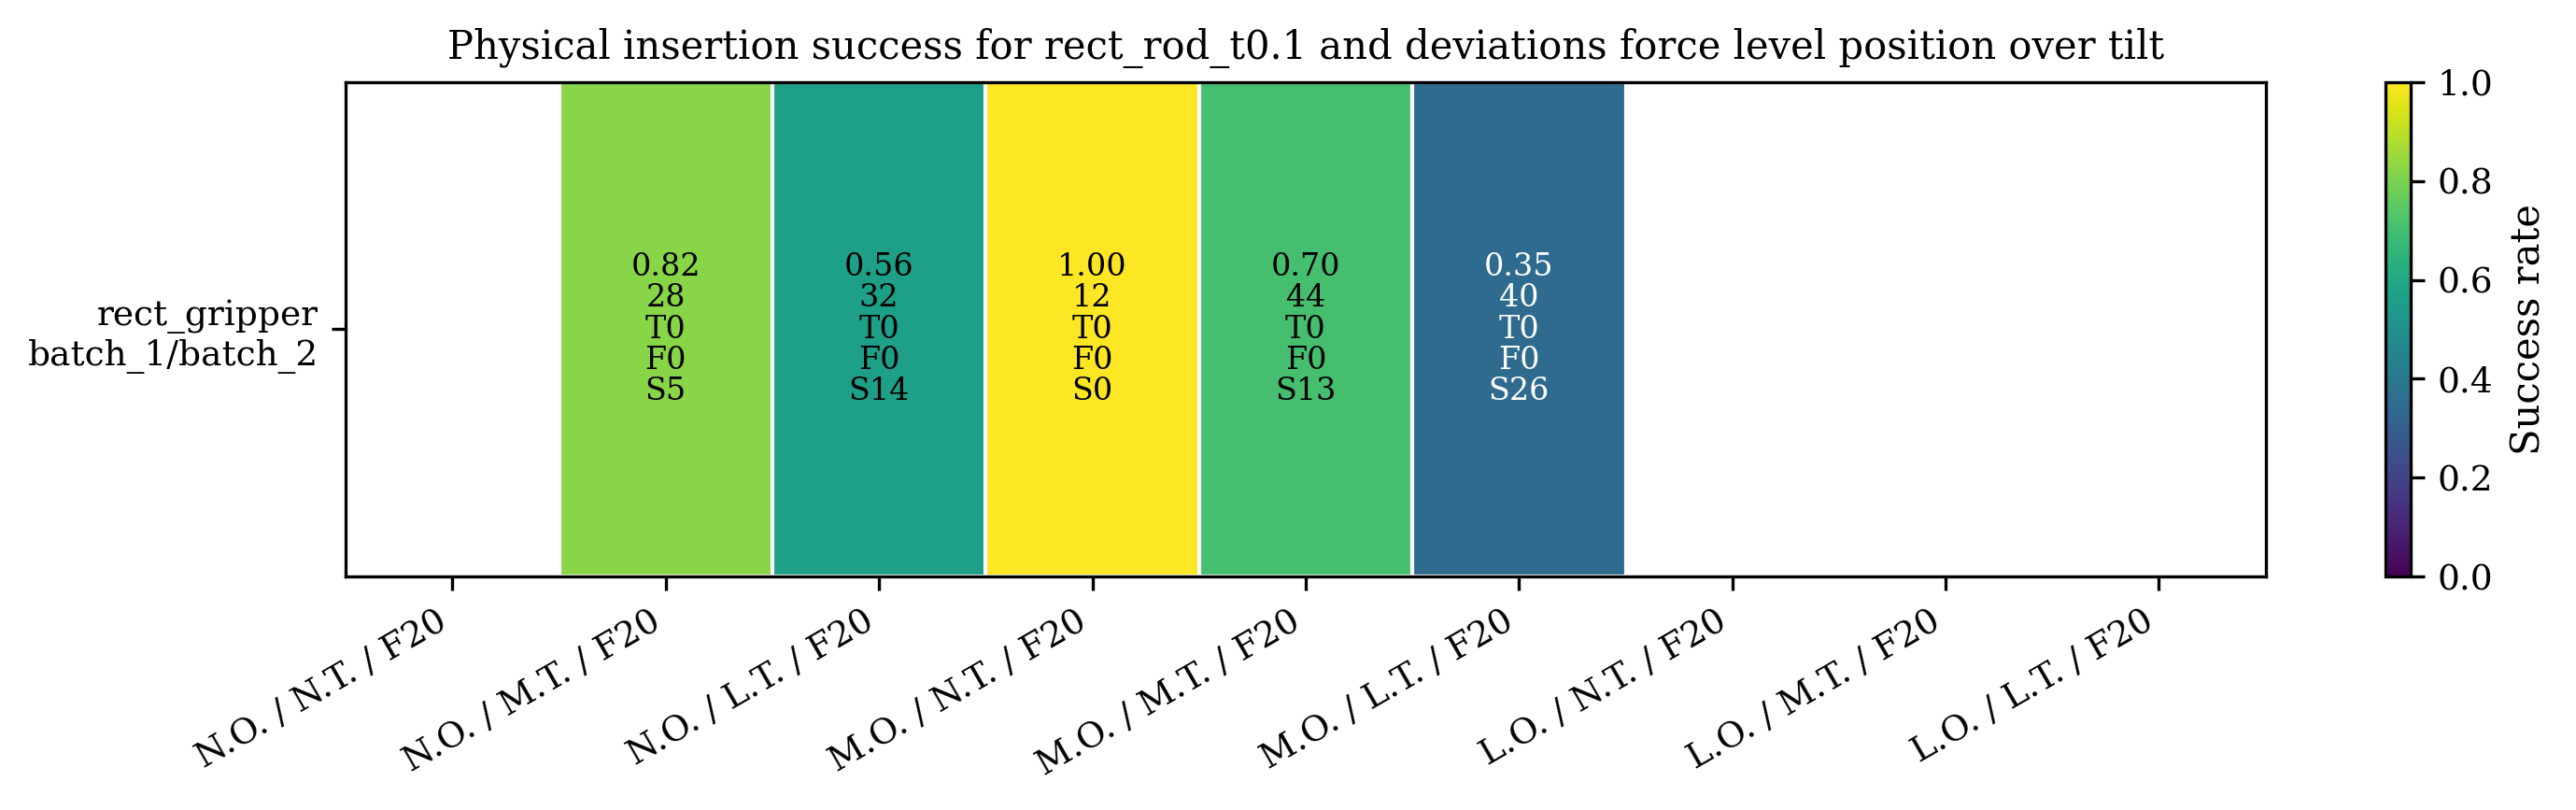
\includegraphics[width=0.95\linewidth]{chapters/7-results/DA1/domain/physical_rect_rod_t0.1_domains_force_level_6.png}
%     \caption{Detailed physical success rate of combined position--tilt groups for selected force levels in \texttt{rect\_rod\_t0.1}. This plot is used to inspect whether force-interaction differences are coupled to geometric deviations.}
%     \label{fig:da1_rect_rod_t01_position_tilt_force_check}
% \end{figure}

% \subsubsection{Summary of Deviation Analysis I}

% The physical success-rate analysis shows that tilt magnitude and force interaction are the most informative global deviation groups. Tilt is associated with a clear reduction in success rate, while radial position offset alone is less systematic. The combined position--tilt analysis confirms that position offset becomes more meaningful when interpreted together with tilt.

% The domain-specific analysis refines this result. Across hole domains, the no-tilt groups are generally more successful than large-tilt groups, but individual hole domains show additional behavior that is hidden in the global plots. The \texttt{small\_rod\_t0.3} domain reveals a directional bias, where negative $x$ and negative $y$ offsets are substantially less successful than positive directions. This suggests a correctable offset in the nominal insertion pose and demonstrates that the metadata analysis can also be used to diagnose the physical robotic setup.

% The \texttt{rect\_rod\_t0.1} investigation shows that force-interaction effects are strongly influenced by failure mode and deterministic coupling in the deviation planner. Low or negative force differences often produce force-limit failures, low commanded force can lead to timeouts, and high limits can allow stall/jam failures. Therefore, force interaction is physically meaningful, but individual force-interaction cells cannot always be interpreted independently from the associated position and tilt deviations.

% Overall, Deviation Analysis I shows that the dataset contains meaningful physical structure beyond the binary success label. The analysis identifies which deviations are associated with insertion failures and reveals domain-specific effects that can guide improvements of the physical insertion process. These results also provide the basis for Deviation Analysis II, where the same deviation groups are analyzed with respect to model confusion rather than physical success rate.

\section{Deviation Analysis II: Model Confusion}
\label{subsec:results_deviation_analysis_2}

\section{Summary of Main Findings}
\label{sec:results_summary}